\documentclass[twoside]{book}

% Packages required by doxygen
\usepackage{fixltx2e}
\usepackage{calc}
\usepackage{doxygen}
\usepackage{graphicx}
\usepackage[utf8]{inputenc}
\usepackage{makeidx}
\usepackage{multicol}
\usepackage{multirow}
\PassOptionsToPackage{warn}{textcomp}
\usepackage{textcomp}
\usepackage[nointegrals]{wasysym}
\usepackage[table]{xcolor}

% Font selection
\usepackage[T1]{fontenc}
\usepackage{mathptmx}
\usepackage[scaled=.90]{helvet}
\usepackage{courier}
\usepackage{amssymb}
\usepackage{sectsty}
\renewcommand{\familydefault}{\sfdefault}
\allsectionsfont{%
  \fontseries{bc}\selectfont%
  \color{darkgray}%
}
\renewcommand{\DoxyLabelFont}{%
  \fontseries{bc}\selectfont%
  \color{darkgray}%
}
\newcommand{\+}{\discretionary{\mbox{\scriptsize$\hookleftarrow$}}{}{}}

% Page & text layout
\usepackage{geometry}
\geometry{%
  a4paper,%
  top=2.5cm,%
  bottom=2.5cm,%
  left=2.5cm,%
  right=2.5cm%
}
\tolerance=750
\hfuzz=15pt
\hbadness=750
\setlength{\emergencystretch}{15pt}
\setlength{\parindent}{0cm}
\setlength{\parskip}{0.2cm}
\makeatletter
\renewcommand{\paragraph}{%
  \@startsection{paragraph}{4}{0ex}{-1.0ex}{1.0ex}{%
    \normalfont\normalsize\bfseries\SS@parafont%
  }%
}
\renewcommand{\subparagraph}{%
  \@startsection{subparagraph}{5}{0ex}{-1.0ex}{1.0ex}{%
    \normalfont\normalsize\bfseries\SS@subparafont%
  }%
}
\makeatother

% Headers & footers
\usepackage{fancyhdr}
\pagestyle{fancyplain}
\fancyhead[LE]{\fancyplain{}{\bfseries\thepage}}
\fancyhead[CE]{\fancyplain{}{}}
\fancyhead[RE]{\fancyplain{}{\bfseries\leftmark}}
\fancyhead[LO]{\fancyplain{}{\bfseries\rightmark}}
\fancyhead[CO]{\fancyplain{}{}}
\fancyhead[RO]{\fancyplain{}{\bfseries\thepage}}
\fancyfoot[LE]{\fancyplain{}{}}
\fancyfoot[CE]{\fancyplain{}{}}
\fancyfoot[RE]{\fancyplain{}{\bfseries\scriptsize Generated on Fri Feb 2 2018 11\+:50\+:17 for Stereo Vision toolkit by Doxygen }}
\fancyfoot[LO]{\fancyplain{}{\bfseries\scriptsize Generated on Fri Feb 2 2018 11\+:50\+:17 for Stereo Vision toolkit by Doxygen }}
\fancyfoot[CO]{\fancyplain{}{}}
\fancyfoot[RO]{\fancyplain{}{}}
\renewcommand{\footrulewidth}{0.4pt}
\renewcommand{\chaptermark}[1]{%
  \markboth{#1}{}%
}
\renewcommand{\sectionmark}[1]{%
  \markright{\thesection\ #1}%
}

% Indices & bibliography
\usepackage{natbib}
\usepackage[titles]{tocloft}
\setcounter{tocdepth}{3}
\setcounter{secnumdepth}{5}
\makeindex

% Hyperlinks (required, but should be loaded last)
\usepackage{ifpdf}
\ifpdf
  \usepackage[pdftex,pagebackref=true]{hyperref}
\else
  \usepackage[ps2pdf,pagebackref=true]{hyperref}
\fi
\hypersetup{%
  colorlinks=true,%
  linkcolor=blue,%
  citecolor=blue,%
  unicode%
}

% Custom commands
\newcommand{\clearemptydoublepage}{%
  \newpage{\pagestyle{empty}\cleardoublepage}%
}


%===== C O N T E N T S =====

\begin{document}

% Titlepage & ToC
\hypersetup{pageanchor=false,
             bookmarks=true,
             bookmarksnumbered=true,
             pdfencoding=unicode
            }
\pagenumbering{roman}
\begin{titlepage}
\vspace*{7cm}
\begin{center}%
{\Large Stereo Vision toolkit }\\
\vspace*{1cm}
{\large Generated by Doxygen 1.8.8}\\
\vspace*{0.5cm}
{\small Fri Feb 2 2018 11:50:17}\\
\end{center}
\end{titlepage}
\clearemptydoublepage
\tableofcontents
\clearemptydoublepage
\pagenumbering{arabic}
\hypersetup{pageanchor=true}

%--- Begin generated contents ---
\chapter{Hierarchical Index}
\section{Class Hierarchy}
This inheritance list is sorted roughly, but not completely, alphabetically\+:\begin{DoxyCompactList}
\item \contentsline{section}{Param\+File}{\pageref{class_param_file}}{}
\item Q\+Dialog\begin{DoxyCompactList}
\item \contentsline{section}{calibrateconfirmdialog}{\pageref{classcalibrateconfirmdialog}}{}
\item \contentsline{section}{Calibrate\+From\+Images\+Dialog}{\pageref{class_calibrate_from_images_dialog}}{}
\item \contentsline{section}{Calibration\+Dialog}{\pageref{class_calibration_dialog}}{}
\end{DoxyCompactList}
\item Q\+Main\+Window\begin{DoxyCompactList}
\item \contentsline{section}{Main\+Window}{\pageref{class_main_window}}{}
\end{DoxyCompactList}
\item Q\+Object\begin{DoxyCompactList}
\item \contentsline{section}{Abstract\+Stereo\+Camera}{\pageref{class_abstract_stereo_camera}}{}
\begin{DoxyCompactList}
\item \contentsline{section}{Stereo\+Camera\+Deimos}{\pageref{class_stereo_camera_deimos}}{}
\item \contentsline{section}{Stereo\+Camera\+From\+Video}{\pageref{class_stereo_camera_from_video}}{}
\item \contentsline{section}{Stereo\+Camera\+Open\+C\+V}{\pageref{class_stereo_camera_open_c_v}}{}
\end{DoxyCompactList}
\item \contentsline{section}{Abstract\+Stereo\+Matcher}{\pageref{class_abstract_stereo_matcher}}{}
\begin{DoxyCompactList}
\item \contentsline{section}{Matcher\+Open\+C\+V\+Block}{\pageref{class_matcher_open_c_v_block}}{}
\item \contentsline{section}{Matcher\+Open\+C\+V\+S\+G\+B\+M}{\pageref{class_matcher_open_c_v_s_g_b_m}}{}
\end{DoxyCompactList}
\item \contentsline{section}{Camera\+Open\+C\+V}{\pageref{class_camera_open_c_v}}{}
\item \contentsline{section}{Chessboard}{\pageref{class_chessboard}}{}
\item \contentsline{section}{Q\+Stereo\+Camera}{\pageref{class_q_stereo_camera}}{}
\item \contentsline{section}{Stereo\+Calibrate}{\pageref{class_stereo_calibrate}}{}
\end{DoxyCompactList}
\item Q\+Widget\begin{DoxyCompactList}
\item \contentsline{section}{Disparity\+Viewer}{\pageref{class_disparity_viewer}}{}
\item \contentsline{section}{Matcher\+Widget}{\pageref{class_matcher_widget}}{}
\begin{DoxyCompactList}
\item \contentsline{section}{Matcher\+Widget\+Open\+C\+V\+Block}{\pageref{class_matcher_widget_open_c_v_block}}{}
\item \contentsline{section}{Matcher\+Widget\+Open\+C\+V\+S\+G\+B\+M}{\pageref{class_matcher_widget_open_c_v_s_g_b_m}}{}
\end{DoxyCompactList}
\end{DoxyCompactList}
\end{DoxyCompactList}

\chapter{Class Index}
\section{Class List}
Here are the classes, structs, unions and interfaces with brief descriptions\+:\begin{DoxyCompactList}
\item\contentsline{section}{\hyperlink{class_abstract_stereo_camera}{Abstract\+Stereo\+Camera} }{\pageref{class_abstract_stereo_camera}}{}
\item\contentsline{section}{\hyperlink{class_abstract_stereo_matcher}{Abstract\+Stereo\+Matcher} }{\pageref{class_abstract_stereo_matcher}}{}
\item\contentsline{section}{\hyperlink{classcalibrateconfirmdialog}{calibrateconfirmdialog} }{\pageref{classcalibrateconfirmdialog}}{}
\item\contentsline{section}{\hyperlink{class_calibrate_from_images_dialog}{Calibrate\+From\+Images\+Dialog} }{\pageref{class_calibrate_from_images_dialog}}{}
\item\contentsline{section}{\hyperlink{class_calibration_dialog}{Calibration\+Dialog} }{\pageref{class_calibration_dialog}}{}
\item\contentsline{section}{\hyperlink{class_camera_open_c_v}{Camera\+Open\+C\+V} }{\pageref{class_camera_open_c_v}}{}
\item\contentsline{section}{\hyperlink{class_chessboard}{Chessboard} }{\pageref{class_chessboard}}{}
\item\contentsline{section}{\hyperlink{class_disparity_viewer}{Disparity\+Viewer} }{\pageref{class_disparity_viewer}}{}
\item\contentsline{section}{\hyperlink{class_main_window}{Main\+Window} }{\pageref{class_main_window}}{}
\item\contentsline{section}{\hyperlink{class_matcher_open_c_v_block}{Matcher\+Open\+C\+V\+Block} }{\pageref{class_matcher_open_c_v_block}}{}
\item\contentsline{section}{\hyperlink{class_matcher_open_c_v_s_g_b_m}{Matcher\+Open\+C\+V\+S\+G\+B\+M} }{\pageref{class_matcher_open_c_v_s_g_b_m}}{}
\item\contentsline{section}{\hyperlink{class_matcher_widget}{Matcher\+Widget} }{\pageref{class_matcher_widget}}{}
\item\contentsline{section}{\hyperlink{class_matcher_widget_open_c_v_block}{Matcher\+Widget\+Open\+C\+V\+Block} }{\pageref{class_matcher_widget_open_c_v_block}}{}
\item\contentsline{section}{\hyperlink{class_matcher_widget_open_c_v_s_g_b_m}{Matcher\+Widget\+Open\+C\+V\+S\+G\+B\+M} }{\pageref{class_matcher_widget_open_c_v_s_g_b_m}}{}
\item\contentsline{section}{\hyperlink{class_param_file}{Param\+File} }{\pageref{class_param_file}}{}
\item\contentsline{section}{\hyperlink{class_q_stereo_camera}{Q\+Stereo\+Camera} }{\pageref{class_q_stereo_camera}}{}
\item\contentsline{section}{\hyperlink{class_stereo_calibrate}{Stereo\+Calibrate} }{\pageref{class_stereo_calibrate}}{}
\item\contentsline{section}{\hyperlink{class_stereo_camera_deimos}{Stereo\+Camera\+Deimos} }{\pageref{class_stereo_camera_deimos}}{}
\item\contentsline{section}{\hyperlink{class_stereo_camera_from_video}{Stereo\+Camera\+From\+Video} }{\pageref{class_stereo_camera_from_video}}{}
\item\contentsline{section}{\hyperlink{class_stereo_camera_open_c_v}{Stereo\+Camera\+Open\+C\+V} }{\pageref{class_stereo_camera_open_c_v}}{}
\end{DoxyCompactList}

\chapter{Class Documentation}
\hypertarget{class_abstract_stereo_camera}{}\section{Abstract\+Stereo\+Camera Class Reference}
\label{class_abstract_stereo_camera}\index{Abstract\+Stereo\+Camera@{Abstract\+Stereo\+Camera}}
Inheritance diagram for Abstract\+Stereo\+Camera\+:\begin{figure}[H]
\begin{center}
\leavevmode
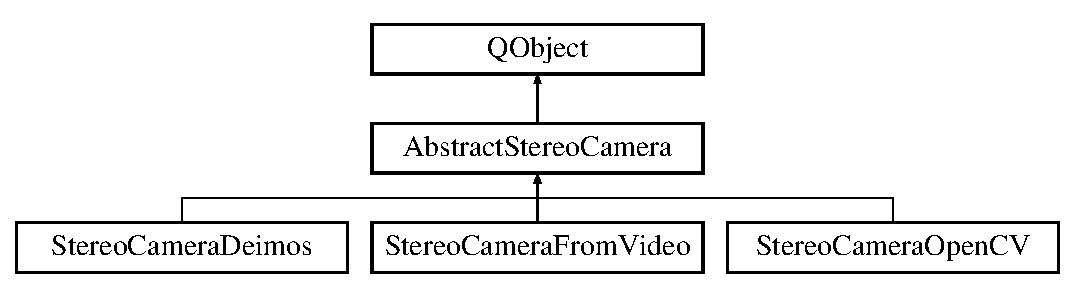
\includegraphics[height=3.000000cm]{class_abstract_stereo_camera}
\end{center}
\end{figure}
\subsection*{Public Slots}
\begin{DoxyCompactItemize}
\item 
\hypertarget{class_abstract_stereo_camera_a1020509400c9e05350211784dd75f8a9}{}void {\bfseries set\+Matcher} (\hyperlink{class_abstract_stereo_matcher}{Abstract\+Stereo\+Matcher} $\ast$matcher)\label{class_abstract_stereo_camera_a1020509400c9e05350211784dd75f8a9}

\item 
bool \hyperlink{class_abstract_stereo_camera_ab4a1141a26a7ba82b6e1b133df41b670}{load\+Calibration} (Q\+String directory)
\begin{DoxyCompactList}\small\item\em Load calibration files from a directory and check them for validity. \end{DoxyCompactList}\item 
\hypertarget{class_abstract_stereo_camera_a11404be55831f47d0954a0c3c9e749b1}{}void \hyperlink{class_abstract_stereo_camera_a11404be55831f47d0954a0c3c9e749b1}{single\+Shot} (void)\label{class_abstract_stereo_camera_a11404be55831f47d0954a0c3c9e749b1}

\begin{DoxyCompactList}\small\item\em Acquire a single frame from the camera and then pause. \end{DoxyCompactList}\item 
\hypertarget{class_abstract_stereo_camera_a3b78f07ba45be840810876cfbe354ce8}{}void \hyperlink{class_abstract_stereo_camera_a3b78f07ba45be840810876cfbe354ce8}{freerun} (void)\label{class_abstract_stereo_camera_a3b78f07ba45be840810876cfbe354ce8}

\begin{DoxyCompactList}\small\item\em Place the camera in freerun mode (continuous acquisition. \end{DoxyCompactList}\item 
\hypertarget{class_abstract_stereo_camera_a0ae4bc133a396a7085b556a62aa9e6f1}{}void \hyperlink{class_abstract_stereo_camera_a0ae4bc133a396a7085b556a62aa9e6f1}{pause} ()\label{class_abstract_stereo_camera_a0ae4bc133a396a7085b556a62aa9e6f1}

\begin{DoxyCompactList}\small\item\em Pause the camera (note this may not actually pause acquisition, but halts frame requests) \end{DoxyCompactList}\item 
virtual bool \hyperlink{class_abstract_stereo_camera_a01d0ecf3cf4bb8e9a6b9e34292483d14}{capture} (void)=0
\begin{DoxyCompactList}\small\item\em Capture an image. \end{DoxyCompactList}\item 
void \hyperlink{class_abstract_stereo_camera_ac299030bbbc8a7445140ca419c94a558}{save\+Image\+Timestamped} ()
\begin{DoxyCompactList}\small\item\em Save an image from the camera with a timestamped filename. \end{DoxyCompactList}\item 
void \hyperlink{class_abstract_stereo_camera_af58b04dd9c17e4d5cc139eb99d738cc6}{video\+Stream\+Start} (Q\+String fname=\char`\"{}\char`\"{})
\begin{DoxyCompactList}\small\item\em Start writing a video stream to a file. \end{DoxyCompactList}\item 
void \hyperlink{class_abstract_stereo_camera_ae39e6f45c68b4bbd4442fdac161051bd}{video\+Stream\+Stop} (void)
\begin{DoxyCompactList}\small\item\em Stop writing a video stream. \end{DoxyCompactList}\item 
\hypertarget{class_abstract_stereo_camera_a1b8bc87de9f73731b0ca1c9b293b57ac}{}void \hyperlink{class_abstract_stereo_camera_a1b8bc87de9f73731b0ca1c9b293b57ac}{enable\+Capture} (bool \hyperlink{class_abstract_stereo_camera_a01d0ecf3cf4bb8e9a6b9e34292483d14}{capture})\label{class_abstract_stereo_camera_a1b8bc87de9f73731b0ca1c9b293b57ac}

\begin{DoxyCompactList}\small\item\em Start or stop capturing an image. \end{DoxyCompactList}\item 
\hypertarget{class_abstract_stereo_camera_aa8bd29dcb39ee696e675087d0c119339}{}void \hyperlink{class_abstract_stereo_camera_aa8bd29dcb39ee696e675087d0c119339}{enable\+Acquire} (bool acquire)\label{class_abstract_stereo_camera_aa8bd29dcb39ee696e675087d0c119339}

\begin{DoxyCompactList}\small\item\em Start or stop capturing images. \end{DoxyCompactList}\item 
\hypertarget{class_abstract_stereo_camera_a0d63f01457d134b1f83d7c6c11e42010}{}void \hyperlink{class_abstract_stereo_camera_a0d63f01457d134b1f83d7c6c11e42010}{enable\+Matching} (bool match)\label{class_abstract_stereo_camera_a0d63f01457d134b1f83d7c6c11e42010}

\begin{DoxyCompactList}\small\item\em Enable or disable stereo matching. \end{DoxyCompactList}\item 
\hypertarget{class_abstract_stereo_camera_a16cb90b828f6f4d4e32a8df9d8b8be0f}{}void \hyperlink{class_abstract_stereo_camera_a16cb90b828f6f4d4e32a8df9d8b8be0f}{enable\+Rectify} (bool rectify)\label{class_abstract_stereo_camera_a16cb90b828f6f4d4e32a8df9d8b8be0f}

\begin{DoxyCompactList}\small\item\em Enable or disable image rectification. \end{DoxyCompactList}\item 
\hypertarget{class_abstract_stereo_camera_ae3dec6f756ff3b6d3702ff3d85e95272}{}void \hyperlink{class_abstract_stereo_camera_ae3dec6f756ff3b6d3702ff3d85e95272}{enable\+Reproject} (bool reproject)\label{class_abstract_stereo_camera_ae3dec6f756ff3b6d3702ff3d85e95272}

\begin{DoxyCompactList}\small\item\em Emable or disable disparity map reprojection to 3\+D. \end{DoxyCompactList}\item 
\hypertarget{class_abstract_stereo_camera_a01c48565e18ae2ac7ea4f3322c2e5059}{}bool \hyperlink{class_abstract_stereo_camera_a01c48565e18ae2ac7ea4f3322c2e5059}{is\+Capturing} ()\label{class_abstract_stereo_camera_a01c48565e18ae2ac7ea4f3322c2e5059}

\begin{DoxyCompactList}\small\item\em Returns whether the camera is currently capturing or processing a frame. \end{DoxyCompactList}\item 
\hypertarget{class_abstract_stereo_camera_a490db3572c901f51f49d90016f856805}{}bool \hyperlink{class_abstract_stereo_camera_a490db3572c901f51f49d90016f856805}{is\+Acquiring} ()\label{class_abstract_stereo_camera_a490db3572c901f51f49d90016f856805}

\begin{DoxyCompactList}\small\item\em Returns whether the camera is currently acquiring images (in general) \end{DoxyCompactList}\item 
\hypertarget{class_abstract_stereo_camera_a0096fcc42b50aa7fa4236f6bddcd81f7}{}bool \hyperlink{class_abstract_stereo_camera_a0096fcc42b50aa7fa4236f6bddcd81f7}{is\+Matching} ()\label{class_abstract_stereo_camera_a0096fcc42b50aa7fa4236f6bddcd81f7}

\begin{DoxyCompactList}\small\item\em Returns whether matching is enabled. \end{DoxyCompactList}\item 
\hypertarget{class_abstract_stereo_camera_a5376ae9c07bdc8e048cbb83a3f11d520}{}bool \hyperlink{class_abstract_stereo_camera_a5376ae9c07bdc8e048cbb83a3f11d520}{is\+Rectifying} ()\label{class_abstract_stereo_camera_a5376ae9c07bdc8e048cbb83a3f11d520}

\begin{DoxyCompactList}\small\item\em Returns whether rectification is being performed. \end{DoxyCompactList}\item 
void \hyperlink{class_abstract_stereo_camera_aa25785c072f75c58b43578c2e718b3c1}{get\+Left\+Image} (cv\+::\+Mat \&dst)
\begin{DoxyCompactList}\small\item\em Get the left stereo image. \end{DoxyCompactList}\item 
void \hyperlink{class_abstract_stereo_camera_aab92c03296efcc915e00cb31016c0c74}{get\+Right\+Image} (cv\+::\+Mat \&dst)
\begin{DoxyCompactList}\small\item\em Get the right stereo image. \end{DoxyCompactList}\item 
cv\+::\+Mat \hyperlink{class_abstract_stereo_camera_abafa9c808e5b2d32cc8e2c9e89fdbb09}{get\+Left\+Image} ()
\begin{DoxyCompactList}\small\item\em Get the left stereo image. \end{DoxyCompactList}\item 
cv\+::\+Mat \hyperlink{class_abstract_stereo_camera_a8b3611b30d65c90128ea59df9e5b9804}{get\+Right\+Image} ()
\begin{DoxyCompactList}\small\item\em Get the right stereo image. \end{DoxyCompactList}\item 
void \hyperlink{class_abstract_stereo_camera_a176f96b1e0cadc210b4a4b73bd51069e}{set\+Visual\+Zmin} (double zmin)
\begin{DoxyCompactList}\small\item\em Set the point cloud clipping distance closest to the camera (i.\+e. specify the closest distance to display) \end{DoxyCompactList}\item 
void \hyperlink{class_abstract_stereo_camera_a5da7d8b7074a30583f22d0efd0af5f28}{set\+Visual\+Zmax} (double zmax)
\begin{DoxyCompactList}\small\item\em Set the point cloud clipping distance furthest from the camera (i.\+e. specify the farthest distance to display) \end{DoxyCompactList}\item 
\hypertarget{class_abstract_stereo_camera_a895b0205fd95e9cd59598d95da7e4b8a}{}void \hyperlink{class_abstract_stereo_camera_a895b0205fd95e9cd59598d95da7e4b8a}{save\+Point\+Cloud} ()\label{class_abstract_stereo_camera_a895b0205fd95e9cd59598d95da7e4b8a}

\begin{DoxyCompactList}\small\item\em Save the current 3\+D reconstruction to a .P\+L\+Y file. \end{DoxyCompactList}\item 
pcl\+::\+Point\+Cloud$<$ pcl\+::\+Point\+X\+Y\+Z\+R\+G\+B $>$\+::Ptr \hyperlink{class_abstract_stereo_camera_ad8f91d2d5e03a466c1066ab27ec3116f}{get\+Point\+Cloud} ()
\begin{DoxyCompactList}\small\item\em Get a pointer to the current point cloud. \end{DoxyCompactList}\item 
int \hyperlink{class_abstract_stereo_camera_a4a1e8d3823219d718f43d5859bfc5096}{get\+Width} (void)
\begin{DoxyCompactList}\small\item\em Get the image width. \end{DoxyCompactList}\item 
int \hyperlink{class_abstract_stereo_camera_ac0918099d91f7ed95f7897610d4aa8a5}{get\+Height} (void)
\begin{DoxyCompactList}\small\item\em Get the image height. \end{DoxyCompactList}\item 
cv\+::\+Size \hyperlink{class_abstract_stereo_camera_a1f35feaeb739af86eb89a25ad58870e4}{get\+Size} (void)
\begin{DoxyCompactList}\small\item\em Get the image size. \end{DoxyCompactList}\item 
void \hyperlink{class_abstract_stereo_camera_aad94fb2509d7c36d33eb176c28963991}{set\+Savelocation} (Q\+String dir)
\begin{DoxyCompactList}\small\item\em Set the save directory. \end{DoxyCompactList}\end{DoxyCompactItemize}
\subsection*{Signals}
\begin{DoxyCompactItemize}
\item 
\hypertarget{class_abstract_stereo_camera_a84dad2b829994b2da0cc4c2c9f7000c4}{}void \hyperlink{class_abstract_stereo_camera_a84dad2b829994b2da0cc4c2c9f7000c4}{acquired} ()\label{class_abstract_stereo_camera_a84dad2b829994b2da0cc4c2c9f7000c4}

\begin{DoxyCompactList}\small\item\em Emitted when a frame has been captured and processed. \end{DoxyCompactList}\item 
\hypertarget{class_abstract_stereo_camera_a2c94f041f379bea5a5d2b4e2e5ba0217}{}void \hyperlink{class_abstract_stereo_camera_a2c94f041f379bea5a5d2b4e2e5ba0217}{fps} (qint64)\label{class_abstract_stereo_camera_a2c94f041f379bea5a5d2b4e2e5ba0217}

\begin{DoxyCompactList}\small\item\em Emitted after a frame has been processed to indicate the current framerate. \end{DoxyCompactList}\item 
\hypertarget{class_abstract_stereo_camera_a6eb388b6b235a928d5792d01db3e0654}{}void \hyperlink{class_abstract_stereo_camera_a6eb388b6b235a928d5792d01db3e0654}{saved\+Image} ()\label{class_abstract_stereo_camera_a6eb388b6b235a928d5792d01db3e0654}

\begin{DoxyCompactList}\small\item\em Emitted when an image has been saved. \end{DoxyCompactList}\item 
\hypertarget{class_abstract_stereo_camera_ae7cf0a8b94f4ee9bba33d8f6fc1d2be0}{}void \hyperlink{class_abstract_stereo_camera_ae7cf0a8b94f4ee9bba33d8f6fc1d2be0}{finished} ()\label{class_abstract_stereo_camera_ae7cf0a8b94f4ee9bba33d8f6fc1d2be0}

\begin{DoxyCompactList}\small\item\em Indicates that the camera has finished acquiring. \end{DoxyCompactList}\item 
\hypertarget{class_abstract_stereo_camera_a23d9368ea4cf1fcac6da6c2b153694d3}{}void \hyperlink{class_abstract_stereo_camera_a23d9368ea4cf1fcac6da6c2b153694d3}{framecount} (qint64)\label{class_abstract_stereo_camera_a23d9368ea4cf1fcac6da6c2b153694d3}

\begin{DoxyCompactList}\small\item\em Indicates the current frame count. \end{DoxyCompactList}\item 
\hypertarget{class_abstract_stereo_camera_a1e8a9c0d394e1efe15ab8189ec3e2597}{}void \hyperlink{class_abstract_stereo_camera_a1e8a9c0d394e1efe15ab8189ec3e2597}{saved\+Image} (Q\+String filename)\label{class_abstract_stereo_camera_a1e8a9c0d394e1efe15ab8189ec3e2597}

\begin{DoxyCompactList}\small\item\em Emit when an image has been saved, including the filename. \end{DoxyCompactList}\item 
\hypertarget{class_abstract_stereo_camera_ac24eaa1c0c62dae96a176f0eac053414}{}void \hyperlink{class_abstract_stereo_camera_ac24eaa1c0c62dae96a176f0eac053414}{matched} ()\label{class_abstract_stereo_camera_ac24eaa1c0c62dae96a176f0eac053414}

\begin{DoxyCompactList}\small\item\em Emitted when an image has been matched. \end{DoxyCompactList}\item 
\hypertarget{class_abstract_stereo_camera_a955561b40fdaeaf218e32fb117b6aa9b}{}void \hyperlink{class_abstract_stereo_camera_a955561b40fdaeaf218e32fb117b6aa9b}{reprojected} ()\label{class_abstract_stereo_camera_a955561b40fdaeaf218e32fb117b6aa9b}

\begin{DoxyCompactList}\small\item\em Emitted when a disparity map has been reprojected to a point cloud. \end{DoxyCompactList}\item 
\hypertarget{class_abstract_stereo_camera_a28c67fb287ceef7cac927595959f5375}{}void \hyperlink{class_abstract_stereo_camera_a28c67fb287ceef7cac927595959f5375}{captured} ()\label{class_abstract_stereo_camera_a28c67fb287ceef7cac927595959f5375}

\begin{DoxyCompactList}\small\item\em Emitted when a camera has captured an image, typically used in sub-\/classes. \end{DoxyCompactList}\item 
\hypertarget{class_abstract_stereo_camera_ae5165b33283bb368413543aeb863bf88}{}void \hyperlink{class_abstract_stereo_camera_ae5165b33283bb368413543aeb863bf88}{have\+Cuda} ()\label{class_abstract_stereo_camera_ae5165b33283bb368413543aeb863bf88}

\begin{DoxyCompactList}\small\item\em Emitted if the host system is found to have a C\+U\+D\+A-\/capable graphics card installed. \end{DoxyCompactList}\item 
\hypertarget{class_abstract_stereo_camera_ab661978020170e7d58906a96ec2fe61e}{}void \hyperlink{class_abstract_stereo_camera_ab661978020170e7d58906a96ec2fe61e}{temperature\+\_\+\+C} (double)\label{class_abstract_stereo_camera_ab661978020170e7d58906a96ec2fe61e}

\begin{DoxyCompactList}\small\item\em Indicates the internal temperature of the camera in Celcius. \end{DoxyCompactList}\end{DoxyCompactItemize}
\subsection*{Public Member Functions}
\begin{DoxyCompactItemize}
\item 
\hypertarget{class_abstract_stereo_camera_ac1e2dcd62f1f8b1478b16bf908ac2721}{}{\bfseries Abstract\+Stereo\+Camera} (Q\+Object $\ast$parent=0)\label{class_abstract_stereo_camera_ac1e2dcd62f1f8b1478b16bf908ac2721}

\item 
void \hyperlink{class_abstract_stereo_camera_a5496f7e9e10c2892d62091dd56709e7a}{assign\+Thread} (Q\+Thread $\ast$thread)
\begin{DoxyCompactList}\small\item\em Assign the stereo camera object to a thread so as not to block the G\+U\+I. Typically called just after instantiation. \end{DoxyCompactList}\end{DoxyCompactItemize}
\subsection*{Public Attributes}
\begin{DoxyCompactItemize}
\item 
\hypertarget{class_abstract_stereo_camera_a9b06e4ac7c5452615f718f76da64681b}{}cv\+::\+Mat {\bfseries left\+\_\+remapped}\label{class_abstract_stereo_camera_a9b06e4ac7c5452615f718f76da64681b}

\item 
\hypertarget{class_abstract_stereo_camera_abf60a27f63d9b0aea7c4069da14fafc4}{}cv\+::\+Mat {\bfseries right\+\_\+remapped}\label{class_abstract_stereo_camera_abf60a27f63d9b0aea7c4069da14fafc4}

\item 
\hypertarget{class_abstract_stereo_camera_a9f3acb606a0e664a1a90877ed2c913a6}{}cv\+::\+Mat {\bfseries left\+\_\+raw}\label{class_abstract_stereo_camera_a9f3acb606a0e664a1a90877ed2c913a6}

\item 
\hypertarget{class_abstract_stereo_camera_a7f7c5484679ac56a23948a9f2cede212}{}cv\+::\+Mat {\bfseries right\+\_\+raw}\label{class_abstract_stereo_camera_a7f7c5484679ac56a23948a9f2cede212}

\item 
\hypertarget{class_abstract_stereo_camera_a97a0d9c267e030634bcd8618ad2966c3}{}cv\+::\+Mat {\bfseries Q}\label{class_abstract_stereo_camera_a97a0d9c267e030634bcd8618ad2966c3}

\item 
\hypertarget{class_abstract_stereo_camera_a7a56c181a09b21a07a389a68cab065a2}{}cv\+::\+Mat {\bfseries stereo\+\_\+reprojected}\label{class_abstract_stereo_camera_a7a56c181a09b21a07a389a68cab065a2}

\end{DoxyCompactItemize}
\subsection*{Protected Attributes}
\begin{DoxyCompactItemize}
\item 
\hypertarget{class_abstract_stereo_camera_ae7facc8693fc536cd62d0c3513f65ae1}{}int {\bfseries frame\+\_\+rate} = 30\label{class_abstract_stereo_camera_ae7facc8693fc536cd62d0c3513f65ae1}

\item 
\hypertarget{class_abstract_stereo_camera_a31d42714c8aafc3708051752bac5266a}{}int {\bfseries image\+\_\+width} = 0\label{class_abstract_stereo_camera_a31d42714c8aafc3708051752bac5266a}

\item 
\hypertarget{class_abstract_stereo_camera_a3b63f57eb44274ec09b6854e0ac4c831}{}int {\bfseries image\+\_\+height} = 0\label{class_abstract_stereo_camera_a3b63f57eb44274ec09b6854e0ac4c831}

\item 
\hypertarget{class_abstract_stereo_camera_a3194fe3b665c6ad61a2cdf0e56b9d58a}{}cv\+::\+Size {\bfseries image\+\_\+size}\label{class_abstract_stereo_camera_a3194fe3b665c6ad61a2cdf0e56b9d58a}

\item 
\hypertarget{class_abstract_stereo_camera_a2c916eeb832136104dfa3cd625966b28}{}bool {\bfseries rectification\+\_\+valid} = false\label{class_abstract_stereo_camera_a2c916eeb832136104dfa3cd625966b28}

\item 
\hypertarget{class_abstract_stereo_camera_aba9b93d70b25aef90dd5f00a0f00ca8a}{}bool {\bfseries calibration\+\_\+valid} = false\label{class_abstract_stereo_camera_aba9b93d70b25aef90dd5f00a0f00ca8a}

\item 
\hypertarget{class_abstract_stereo_camera_aa91b2dff7505fca206087c9559a0625b}{}bool {\bfseries connected} = false\label{class_abstract_stereo_camera_aa91b2dff7505fca206087c9559a0625b}

\end{DoxyCompactItemize}


\subsection{Detailed Description}


Definition at line 32 of file abstractstereocamera.\+h.



\subsection{Member Function Documentation}
\hypertarget{class_abstract_stereo_camera_a5496f7e9e10c2892d62091dd56709e7a}{}\index{Abstract\+Stereo\+Camera@{Abstract\+Stereo\+Camera}!assign\+Thread@{assign\+Thread}}
\index{assign\+Thread@{assign\+Thread}!Abstract\+Stereo\+Camera@{Abstract\+Stereo\+Camera}}
\subsubsection[{assign\+Thread}]{\setlength{\rightskip}{0pt plus 5cm}void Abstract\+Stereo\+Camera\+::assign\+Thread (
\begin{DoxyParamCaption}
\item[{Q\+Thread $\ast$}]{thread}
\end{DoxyParamCaption}
)}\label{class_abstract_stereo_camera_a5496f7e9e10c2892d62091dd56709e7a}


Assign the stereo camera object to a thread so as not to block the G\+U\+I. Typically called just after instantiation. 


\begin{DoxyParams}[1]{Parameters}
\mbox{\tt in}  & {\em thread} & Pointer to thread \\
\hline
\end{DoxyParams}


Definition at line 17 of file abstractstereocamera.\+cpp.

\hypertarget{class_abstract_stereo_camera_a01d0ecf3cf4bb8e9a6b9e34292483d14}{}\index{Abstract\+Stereo\+Camera@{Abstract\+Stereo\+Camera}!capture@{capture}}
\index{capture@{capture}!Abstract\+Stereo\+Camera@{Abstract\+Stereo\+Camera}}
\subsubsection[{capture}]{\setlength{\rightskip}{0pt plus 5cm}virtual bool Abstract\+Stereo\+Camera\+::capture (
\begin{DoxyParamCaption}
\item[{void}]{}
\end{DoxyParamCaption}
)\hspace{0.3cm}{\ttfamily [pure virtual]}, {\ttfamily [slot]}}\label{class_abstract_stereo_camera_a01d0ecf3cf4bb8e9a6b9e34292483d14}


Capture an image. 

This is a virtual function which should be implmeented by a particular camera driver.

\begin{DoxyReturn}{Returns}
True if an image was captured successfully, false otherwise 
\end{DoxyReturn}


Implemented in \hyperlink{class_stereo_camera_deimos_a7526953f7562acc07841ebd6a49dc043}{Stereo\+Camera\+Deimos}, \hyperlink{class_stereo_camera_open_c_v_ac669e811da12df2bfd76f783c0550100}{Stereo\+Camera\+Open\+C\+V}, and \hyperlink{class_stereo_camera_from_video_af53503df1755c0a9cf84718128ed0a5d}{Stereo\+Camera\+From\+Video}.

\hypertarget{class_abstract_stereo_camera_ac0918099d91f7ed95f7897610d4aa8a5}{}\index{Abstract\+Stereo\+Camera@{Abstract\+Stereo\+Camera}!get\+Height@{get\+Height}}
\index{get\+Height@{get\+Height}!Abstract\+Stereo\+Camera@{Abstract\+Stereo\+Camera}}
\subsubsection[{get\+Height}]{\setlength{\rightskip}{0pt plus 5cm}int Abstract\+Stereo\+Camera\+::get\+Height (
\begin{DoxyParamCaption}
\item[{void}]{}
\end{DoxyParamCaption}
)\hspace{0.3cm}{\ttfamily [inline]}, {\ttfamily [slot]}}\label{class_abstract_stereo_camera_ac0918099d91f7ed95f7897610d4aa8a5}


Get the image height. 

\begin{DoxyReturn}{Returns}
Image height 
\end{DoxyReturn}


Definition at line 222 of file abstractstereocamera.\+h.

\hypertarget{class_abstract_stereo_camera_aa25785c072f75c58b43578c2e718b3c1}{}\index{Abstract\+Stereo\+Camera@{Abstract\+Stereo\+Camera}!get\+Left\+Image@{get\+Left\+Image}}
\index{get\+Left\+Image@{get\+Left\+Image}!Abstract\+Stereo\+Camera@{Abstract\+Stereo\+Camera}}
\subsubsection[{get\+Left\+Image}]{\setlength{\rightskip}{0pt plus 5cm}void Abstract\+Stereo\+Camera\+::get\+Left\+Image (
\begin{DoxyParamCaption}
\item[{cv\+::\+Mat \&}]{dst}
\end{DoxyParamCaption}
)\hspace{0.3cm}{\ttfamily [slot]}}\label{class_abstract_stereo_camera_aa25785c072f75c58b43578c2e718b3c1}


Get the left stereo image. 


\begin{DoxyParams}[1]{Parameters}
\mbox{\tt out}  & {\em dst} & Open\+C\+V matrix to store image into \\
\hline
\end{DoxyParams}


Definition at line 202 of file abstractstereocamera.\+cpp.

\hypertarget{class_abstract_stereo_camera_abafa9c808e5b2d32cc8e2c9e89fdbb09}{}\index{Abstract\+Stereo\+Camera@{Abstract\+Stereo\+Camera}!get\+Left\+Image@{get\+Left\+Image}}
\index{get\+Left\+Image@{get\+Left\+Image}!Abstract\+Stereo\+Camera@{Abstract\+Stereo\+Camera}}
\subsubsection[{get\+Left\+Image}]{\setlength{\rightskip}{0pt plus 5cm}cv\+::\+Mat Abstract\+Stereo\+Camera\+::get\+Left\+Image (
\begin{DoxyParamCaption}
\item[{void}]{}
\end{DoxyParamCaption}
)\hspace{0.3cm}{\ttfamily [slot]}}\label{class_abstract_stereo_camera_abafa9c808e5b2d32cc8e2c9e89fdbb09}


Get the left stereo image. 

\begin{DoxyReturn}{Returns}
Open\+C\+V matrix containing left image 
\end{DoxyReturn}


Definition at line 210 of file abstractstereocamera.\+cpp.

\hypertarget{class_abstract_stereo_camera_ad8f91d2d5e03a466c1066ab27ec3116f}{}\index{Abstract\+Stereo\+Camera@{Abstract\+Stereo\+Camera}!get\+Point\+Cloud@{get\+Point\+Cloud}}
\index{get\+Point\+Cloud@{get\+Point\+Cloud}!Abstract\+Stereo\+Camera@{Abstract\+Stereo\+Camera}}
\subsubsection[{get\+Point\+Cloud}]{\setlength{\rightskip}{0pt plus 5cm}pcl\+::\+Point\+Cloud$<$ pcl\+::\+Point\+X\+Y\+Z\+R\+G\+B $>$\+::Ptr Abstract\+Stereo\+Camera\+::get\+Point\+Cloud (
\begin{DoxyParamCaption}
{}
\end{DoxyParamCaption}
)\hspace{0.3cm}{\ttfamily [slot]}}\label{class_abstract_stereo_camera_ad8f91d2d5e03a466c1066ab27ec3116f}


Get a pointer to the current point cloud. 

\begin{DoxyReturn}{Returns}
Pointer to the current point cloud 
\end{DoxyReturn}


Definition at line 165 of file abstractstereocamera.\+cpp.

\hypertarget{class_abstract_stereo_camera_aab92c03296efcc915e00cb31016c0c74}{}\index{Abstract\+Stereo\+Camera@{Abstract\+Stereo\+Camera}!get\+Right\+Image@{get\+Right\+Image}}
\index{get\+Right\+Image@{get\+Right\+Image}!Abstract\+Stereo\+Camera@{Abstract\+Stereo\+Camera}}
\subsubsection[{get\+Right\+Image}]{\setlength{\rightskip}{0pt plus 5cm}void Abstract\+Stereo\+Camera\+::get\+Right\+Image (
\begin{DoxyParamCaption}
\item[{cv\+::\+Mat \&}]{dst}
\end{DoxyParamCaption}
)\hspace{0.3cm}{\ttfamily [slot]}}\label{class_abstract_stereo_camera_aab92c03296efcc915e00cb31016c0c74}


Get the right stereo image. 


\begin{DoxyParams}[1]{Parameters}
\mbox{\tt out}  & {\em dst} & Open\+C\+V matrix to store image into \\
\hline
\end{DoxyParams}


Definition at line 206 of file abstractstereocamera.\+cpp.

\hypertarget{class_abstract_stereo_camera_a8b3611b30d65c90128ea59df9e5b9804}{}\index{Abstract\+Stereo\+Camera@{Abstract\+Stereo\+Camera}!get\+Right\+Image@{get\+Right\+Image}}
\index{get\+Right\+Image@{get\+Right\+Image}!Abstract\+Stereo\+Camera@{Abstract\+Stereo\+Camera}}
\subsubsection[{get\+Right\+Image}]{\setlength{\rightskip}{0pt plus 5cm}cv\+::\+Mat Abstract\+Stereo\+Camera\+::get\+Right\+Image (
\begin{DoxyParamCaption}
\item[{void}]{}
\end{DoxyParamCaption}
)\hspace{0.3cm}{\ttfamily [slot]}}\label{class_abstract_stereo_camera_a8b3611b30d65c90128ea59df9e5b9804}


Get the right stereo image. 

\begin{DoxyReturn}{Returns}
Open\+C\+V matrix containing right image 
\end{DoxyReturn}


Definition at line 212 of file abstractstereocamera.\+cpp.

\hypertarget{class_abstract_stereo_camera_a1f35feaeb739af86eb89a25ad58870e4}{}\index{Abstract\+Stereo\+Camera@{Abstract\+Stereo\+Camera}!get\+Size@{get\+Size}}
\index{get\+Size@{get\+Size}!Abstract\+Stereo\+Camera@{Abstract\+Stereo\+Camera}}
\subsubsection[{get\+Size}]{\setlength{\rightskip}{0pt plus 5cm}cv\+::\+Size Abstract\+Stereo\+Camera\+::get\+Size (
\begin{DoxyParamCaption}
\item[{void}]{}
\end{DoxyParamCaption}
)\hspace{0.3cm}{\ttfamily [inline]}, {\ttfamily [slot]}}\label{class_abstract_stereo_camera_a1f35feaeb739af86eb89a25ad58870e4}


Get the image size. 

\begin{DoxyReturn}{Returns}
Image size 
\end{DoxyReturn}


Definition at line 228 of file abstractstereocamera.\+h.

\hypertarget{class_abstract_stereo_camera_a4a1e8d3823219d718f43d5859bfc5096}{}\index{Abstract\+Stereo\+Camera@{Abstract\+Stereo\+Camera}!get\+Width@{get\+Width}}
\index{get\+Width@{get\+Width}!Abstract\+Stereo\+Camera@{Abstract\+Stereo\+Camera}}
\subsubsection[{get\+Width}]{\setlength{\rightskip}{0pt plus 5cm}int Abstract\+Stereo\+Camera\+::get\+Width (
\begin{DoxyParamCaption}
\item[{void}]{}
\end{DoxyParamCaption}
)\hspace{0.3cm}{\ttfamily [inline]}, {\ttfamily [slot]}}\label{class_abstract_stereo_camera_a4a1e8d3823219d718f43d5859bfc5096}


Get the image width. 

\begin{DoxyReturn}{Returns}
Image width 
\end{DoxyReturn}


Definition at line 216 of file abstractstereocamera.\+h.

\hypertarget{class_abstract_stereo_camera_ab4a1141a26a7ba82b6e1b133df41b670}{}\index{Abstract\+Stereo\+Camera@{Abstract\+Stereo\+Camera}!load\+Calibration@{load\+Calibration}}
\index{load\+Calibration@{load\+Calibration}!Abstract\+Stereo\+Camera@{Abstract\+Stereo\+Camera}}
\subsubsection[{load\+Calibration}]{\setlength{\rightskip}{0pt plus 5cm}bool Abstract\+Stereo\+Camera\+::load\+Calibration (
\begin{DoxyParamCaption}
\item[{Q\+String}]{directory}
\end{DoxyParamCaption}
)\hspace{0.3cm}{\ttfamily [slot]}}\label{class_abstract_stereo_camera_ab4a1141a26a7ba82b6e1b133df41b670}


Load calibration files from a directory and check them for validity. 


\begin{DoxyParams}[1]{Parameters}
\mbox{\tt in}  & {\em directory} & The folder too check. \\
\hline
\end{DoxyParams}
\begin{DoxyReturn}{Returns}
True or false, depending on whether the parameters are valid. 
\end{DoxyReturn}


Definition at line 241 of file abstractstereocamera.\+cpp.

\hypertarget{class_abstract_stereo_camera_ac299030bbbc8a7445140ca419c94a558}{}\index{Abstract\+Stereo\+Camera@{Abstract\+Stereo\+Camera}!save\+Image\+Timestamped@{save\+Image\+Timestamped}}
\index{save\+Image\+Timestamped@{save\+Image\+Timestamped}!Abstract\+Stereo\+Camera@{Abstract\+Stereo\+Camera}}
\subsubsection[{save\+Image\+Timestamped}]{\setlength{\rightskip}{0pt plus 5cm}void Abstract\+Stereo\+Camera\+::save\+Image\+Timestamped (
\begin{DoxyParamCaption}
\item[{void}]{}
\end{DoxyParamCaption}
)\hspace{0.3cm}{\ttfamily [slot]}}\label{class_abstract_stereo_camera_ac299030bbbc8a7445140ca419c94a558}


Save an image from the camera with a timestamped filename. 

The timestamp format is\+: yyyy\+M\+Mdd\+\_\+hhmmss\+\_\+zzz (year, month, day, hour, minute, second, millisecond)

\begin{DoxySeeAlso}{See also}
\hyperlink{class_abstract_stereo_camera_aad94fb2509d7c36d33eb176c28963991}{set\+Savelocation()} 
\end{DoxySeeAlso}


Definition at line 25 of file abstractstereocamera.\+cpp.

\hypertarget{class_abstract_stereo_camera_aad94fb2509d7c36d33eb176c28963991}{}\index{Abstract\+Stereo\+Camera@{Abstract\+Stereo\+Camera}!set\+Savelocation@{set\+Savelocation}}
\index{set\+Savelocation@{set\+Savelocation}!Abstract\+Stereo\+Camera@{Abstract\+Stereo\+Camera}}
\subsubsection[{set\+Savelocation}]{\setlength{\rightskip}{0pt plus 5cm}void Abstract\+Stereo\+Camera\+::set\+Savelocation (
\begin{DoxyParamCaption}
\item[{Q\+String}]{dir}
\end{DoxyParamCaption}
)\hspace{0.3cm}{\ttfamily [inline]}, {\ttfamily [slot]}}\label{class_abstract_stereo_camera_aad94fb2509d7c36d33eb176c28963991}


Set the save directory. 


\begin{DoxyParams}{Parameters}
{\em dir} & Desired save directory, will attempt to create if it doesn't exist. \\
\hline
\end{DoxyParams}


Definition at line 234 of file abstractstereocamera.\+h.

\hypertarget{class_abstract_stereo_camera_a5da7d8b7074a30583f22d0efd0af5f28}{}\index{Abstract\+Stereo\+Camera@{Abstract\+Stereo\+Camera}!set\+Visual\+Zmax@{set\+Visual\+Zmax}}
\index{set\+Visual\+Zmax@{set\+Visual\+Zmax}!Abstract\+Stereo\+Camera@{Abstract\+Stereo\+Camera}}
\subsubsection[{set\+Visual\+Zmax}]{\setlength{\rightskip}{0pt plus 5cm}void Abstract\+Stereo\+Camera\+::set\+Visual\+Zmax (
\begin{DoxyParamCaption}
\item[{double}]{zmax}
\end{DoxyParamCaption}
)\hspace{0.3cm}{\ttfamily [slot]}}\label{class_abstract_stereo_camera_a5da7d8b7074a30583f22d0efd0af5f28}


Set the point cloud clipping distance furthest from the camera (i.\+e. specify the farthest distance to display) 


\begin{DoxyParams}[1]{Parameters}
\mbox{\tt in}  & {\em zmax} & Distance to the camera in metres \\
\hline
\end{DoxyParams}


Definition at line 70 of file abstractstereocamera.\+cpp.

\hypertarget{class_abstract_stereo_camera_a176f96b1e0cadc210b4a4b73bd51069e}{}\index{Abstract\+Stereo\+Camera@{Abstract\+Stereo\+Camera}!set\+Visual\+Zmin@{set\+Visual\+Zmin}}
\index{set\+Visual\+Zmin@{set\+Visual\+Zmin}!Abstract\+Stereo\+Camera@{Abstract\+Stereo\+Camera}}
\subsubsection[{set\+Visual\+Zmin}]{\setlength{\rightskip}{0pt plus 5cm}void Abstract\+Stereo\+Camera\+::set\+Visual\+Zmin (
\begin{DoxyParamCaption}
\item[{double}]{zmin}
\end{DoxyParamCaption}
)\hspace{0.3cm}{\ttfamily [slot]}}\label{class_abstract_stereo_camera_a176f96b1e0cadc210b4a4b73bd51069e}


Set the point cloud clipping distance closest to the camera (i.\+e. specify the closest distance to display) 


\begin{DoxyParams}[1]{Parameters}
\mbox{\tt in}  & {\em zmin} & Distance to the camera in metres \\
\hline
\end{DoxyParams}


Definition at line 63 of file abstractstereocamera.\+cpp.

\hypertarget{class_abstract_stereo_camera_af58b04dd9c17e4d5cc139eb99d738cc6}{}\index{Abstract\+Stereo\+Camera@{Abstract\+Stereo\+Camera}!video\+Stream\+Start@{video\+Stream\+Start}}
\index{video\+Stream\+Start@{video\+Stream\+Start}!Abstract\+Stereo\+Camera@{Abstract\+Stereo\+Camera}}
\subsubsection[{video\+Stream\+Start}]{\setlength{\rightskip}{0pt plus 5cm}void Abstract\+Stereo\+Camera\+::video\+Stream\+Start (
\begin{DoxyParamCaption}
\item[{Q\+String}]{fname = {\ttfamily \char`\"{}\char`\"{}}}
\end{DoxyParamCaption}
)\hspace{0.3cm}{\ttfamily [slot]}}\label{class_abstract_stereo_camera_af58b04dd9c17e4d5cc139eb99d738cc6}


Start writing a video stream to a file. 

If no filename is supplied, a timestamped video will be stored in the current selected save folder.


\begin{DoxyParams}[1]{Parameters}
\mbox{\tt out}  & {\em fname} & The output filename \\
\hline
\end{DoxyParams}
\begin{DoxySeeAlso}{See also}
\hyperlink{class_abstract_stereo_camera_aad94fb2509d7c36d33eb176c28963991}{set\+Savelocation()}, \hyperlink{class_abstract_stereo_camera_ae39e6f45c68b4bbd4442fdac161051bd}{video\+Stream\+Stop()} 
\end{DoxySeeAlso}


Definition at line 431 of file abstractstereocamera.\+cpp.

\hypertarget{class_abstract_stereo_camera_ae39e6f45c68b4bbd4442fdac161051bd}{}\index{Abstract\+Stereo\+Camera@{Abstract\+Stereo\+Camera}!video\+Stream\+Stop@{video\+Stream\+Stop}}
\index{video\+Stream\+Stop@{video\+Stream\+Stop}!Abstract\+Stereo\+Camera@{Abstract\+Stereo\+Camera}}
\subsubsection[{video\+Stream\+Stop}]{\setlength{\rightskip}{0pt plus 5cm}void Abstract\+Stereo\+Camera\+::video\+Stream\+Stop (
\begin{DoxyParamCaption}
\item[{void}]{}
\end{DoxyParamCaption}
)\hspace{0.3cm}{\ttfamily [slot]}}\label{class_abstract_stereo_camera_ae39e6f45c68b4bbd4442fdac161051bd}


Stop writing a video stream. 

\begin{DoxySeeAlso}{See also}
\hyperlink{class_abstract_stereo_camera_af58b04dd9c17e4d5cc139eb99d738cc6}{video\+Stream\+Start()} 
\end{DoxySeeAlso}


Definition at line 487 of file abstractstereocamera.\+cpp.



The documentation for this class was generated from the following files\+:\begin{DoxyCompactItemize}
\item 
src/abstractstereocamera.\+h\item 
src/abstractstereocamera.\+cpp\end{DoxyCompactItemize}

\hypertarget{class_abstract_stereo_matcher}{}\section{Abstract\+Stereo\+Matcher Class Reference}
\label{class_abstract_stereo_matcher}\index{Abstract\+Stereo\+Matcher@{Abstract\+Stereo\+Matcher}}
Inheritance diagram for Abstract\+Stereo\+Matcher\+:\begin{figure}[H]
\begin{center}
\leavevmode
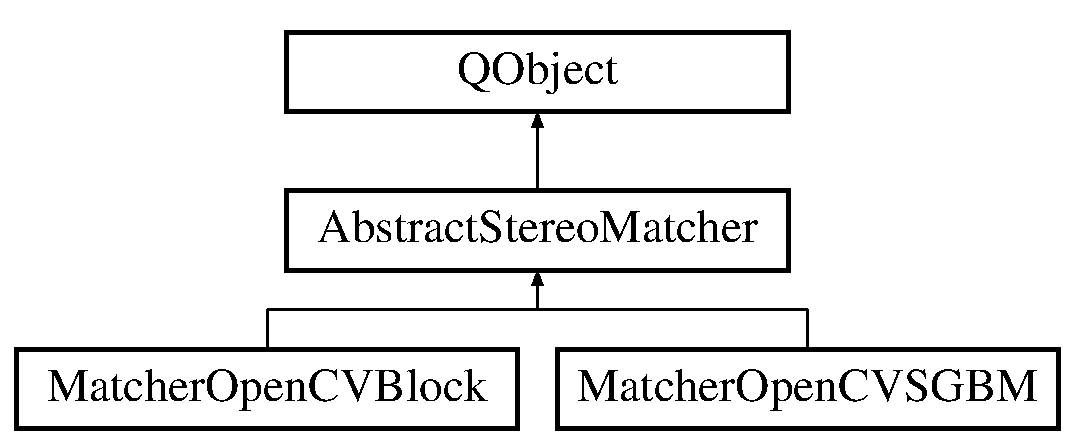
\includegraphics[height=3.000000cm]{class_abstract_stereo_matcher}
\end{center}
\end{figure}
\subsection*{Public Slots}
\begin{DoxyCompactItemize}
\item 
\hypertarget{class_abstract_stereo_matcher_a9d1270578e9ea21b31db33a8e9956675}{}void {\bfseries set\+Images} (cv\+::\+Mat $\ast$left, cv\+::\+Mat $\ast$right)\label{class_abstract_stereo_matcher_a9d1270578e9ea21b31db33a8e9956675}

\item 
\hypertarget{class_abstract_stereo_matcher_aaccfe2a4402687f8a51349976b49c94a}{}virtual void {\bfseries forward\+Match} ()=0\label{class_abstract_stereo_matcher_aaccfe2a4402687f8a51349976b49c94a}

\item 
\hypertarget{class_abstract_stereo_matcher_a4e2bc164538e6dab3d31dcee275031b0}{}virtual void {\bfseries backward\+Match} ()=0\label{class_abstract_stereo_matcher_a4e2bc164538e6dab3d31dcee275031b0}

\item 
\hypertarget{class_abstract_stereo_matcher_afb869f34062416ce17246598e2b77090}{}virtual void {\bfseries init} (void)=0\label{class_abstract_stereo_matcher_afb869f34062416ce17246598e2b77090}

\item 
\hypertarget{class_abstract_stereo_matcher_a87525ed38b36c37d2eda34c0e2d321d7}{}virtual int {\bfseries get\+Error\+Disparity} (void)=0\label{class_abstract_stereo_matcher_a87525ed38b36c37d2eda34c0e2d321d7}

\item 
\hypertarget{class_abstract_stereo_matcher_a124604c16466bac10a308436dd2f07db}{}void {\bfseries assign\+Thread} (Q\+Thread $\ast$thread)\label{class_abstract_stereo_matcher_a124604c16466bac10a308436dd2f07db}

\item 
\hypertarget{class_abstract_stereo_matcher_a2b1a5e9841f39988686450b1f1721032}{}void {\bfseries get\+Disparity} (cv\+::\+Mat \&dst)\label{class_abstract_stereo_matcher_a2b1a5e9841f39988686450b1f1721032}

\item 
\hypertarget{class_abstract_stereo_matcher_a80c14c977bd44695d1142eaef8abdcb3}{}void {\bfseries save\+Disparity} (Q\+String filename)\label{class_abstract_stereo_matcher_a80c14c977bd44695d1142eaef8abdcb3}

\item 
\hypertarget{class_abstract_stereo_matcher_ac89bdb7ff8010eb3cffc22ae73dd5436}{}void {\bfseries check\+L\+R\+Consistency\+Full} (double threshold)\label{class_abstract_stereo_matcher_ac89bdb7ff8010eb3cffc22ae73dd5436}

\item 
\hypertarget{class_abstract_stereo_matcher_a23d41c7aa8ee75b83c0f86028854e92c}{}cv\+::\+Mat $\ast$ {\bfseries get\+Left\+Image} (void)\label{class_abstract_stereo_matcher_a23d41c7aa8ee75b83c0f86028854e92c}

\item 
\hypertarget{class_abstract_stereo_matcher_a3e1d35e2aed668657aa9441c5b563d2d}{}cv\+::\+Mat $\ast$ {\bfseries get\+Rightt\+Image} (void)\label{class_abstract_stereo_matcher_a3e1d35e2aed668657aa9441c5b563d2d}

\item 
\hypertarget{class_abstract_stereo_matcher_a49f42fbfee8266b81fbe17e8af07d73b}{}virtual void {\bfseries match} ()\label{class_abstract_stereo_matcher_a49f42fbfee8266b81fbe17e8af07d73b}

\end{DoxyCompactItemize}
\subsection*{Signals}
\begin{DoxyCompactItemize}
\item 
\hypertarget{class_abstract_stereo_matcher_ab28ce957fa500cd23cf8cfc474294a19}{}void {\bfseries finished} ()\label{class_abstract_stereo_matcher_ab28ce957fa500cd23cf8cfc474294a19}

\end{DoxyCompactItemize}
\subsection*{Public Member Functions}
\begin{DoxyCompactItemize}
\item 
\hypertarget{class_abstract_stereo_matcher_a17362bf0ea979b621a6e71178930b4b0}{}{\bfseries Abstract\+Stereo\+Matcher} (Q\+Object $\ast$parent=0, cv\+::\+Size image\+\_\+size=cv\+::\+Size(0, 0))\label{class_abstract_stereo_matcher_a17362bf0ea979b621a6e71178930b4b0}

\end{DoxyCompactItemize}
\subsection*{Public Attributes}
\begin{DoxyCompactItemize}
\item 
\hypertarget{class_abstract_stereo_matcher_aec41d8677f57e6db0f1851f4067e17dc}{}cv\+::\+Mat {\bfseries disparity\+\_\+lr}\label{class_abstract_stereo_matcher_aec41d8677f57e6db0f1851f4067e17dc}

\end{DoxyCompactItemize}
\subsection*{Protected Attributes}
\begin{DoxyCompactItemize}
\item 
\hypertarget{class_abstract_stereo_matcher_ab588c178d38aefc2bd8fdbb267d58fa3}{}cv\+::\+Mat $\ast$ {\bfseries left}\label{class_abstract_stereo_matcher_ab588c178d38aefc2bd8fdbb267d58fa3}

\item 
\hypertarget{class_abstract_stereo_matcher_a57d8d83507e36de82d29091c662cd7a1}{}cv\+::\+Mat $\ast$ {\bfseries right}\label{class_abstract_stereo_matcher_a57d8d83507e36de82d29091c662cd7a1}

\item 
\hypertarget{class_abstract_stereo_matcher_a8cdb8335cd34ea188acb52af1c61767f}{}cv\+::\+Mat {\bfseries disparity\+\_\+buffer}\label{class_abstract_stereo_matcher_a8cdb8335cd34ea188acb52af1c61767f}

\item 
\hypertarget{class_abstract_stereo_matcher_a51c30315cdc2c2eb0442abfccd99c2a3}{}cv\+::\+Mat {\bfseries disparity\+\_\+rl}\label{class_abstract_stereo_matcher_a51c30315cdc2c2eb0442abfccd99c2a3}

\item 
\hypertarget{class_abstract_stereo_matcher_a9465d0369a736080bdd9466a8eb99e01}{}cv\+::\+Mat {\bfseries disparity\+\_\+scale}\label{class_abstract_stereo_matcher_a9465d0369a736080bdd9466a8eb99e01}

\item 
\hypertarget{class_abstract_stereo_matcher_a923b35821693ae332ca597d1aa39eda6}{}cv\+::\+Size {\bfseries image\+\_\+size}\label{class_abstract_stereo_matcher_a923b35821693ae332ca597d1aa39eda6}

\item 
\hypertarget{class_abstract_stereo_matcher_a34abfc8eae69117a1095aaea88ae757f}{}int {\bfseries min\+\_\+disparity} = 0\label{class_abstract_stereo_matcher_a34abfc8eae69117a1095aaea88ae757f}

\item 
\hypertarget{class_abstract_stereo_matcher_af950cd28dd5ace7e5dda654f85878990}{}int {\bfseries disparity\+\_\+range} = 64\label{class_abstract_stereo_matcher_af950cd28dd5ace7e5dda654f85878990}

\item 
\hypertarget{class_abstract_stereo_matcher_a120960da2f7cb8f7549f359c6ff7e86d}{}int {\bfseries block\+\_\+size} = 9\label{class_abstract_stereo_matcher_a120960da2f7cb8f7549f359c6ff7e86d}

\end{DoxyCompactItemize}


\subsection{Detailed Description}


Definition at line 17 of file abstractstereomatcher.\+h.



The documentation for this class was generated from the following files\+:\begin{DoxyCompactItemize}
\item 
src/abstractstereomatcher.\+h\item 
src/abstractstereomatcher.\+cpp\end{DoxyCompactItemize}

\hypertarget{classcalibrateconfirmdialog}{}\section{calibrateconfirmdialog Class Reference}
\label{classcalibrateconfirmdialog}\index{calibrateconfirmdialog@{calibrateconfirmdialog}}
Inheritance diagram for calibrateconfirmdialog\+:\begin{figure}[H]
\begin{center}
\leavevmode
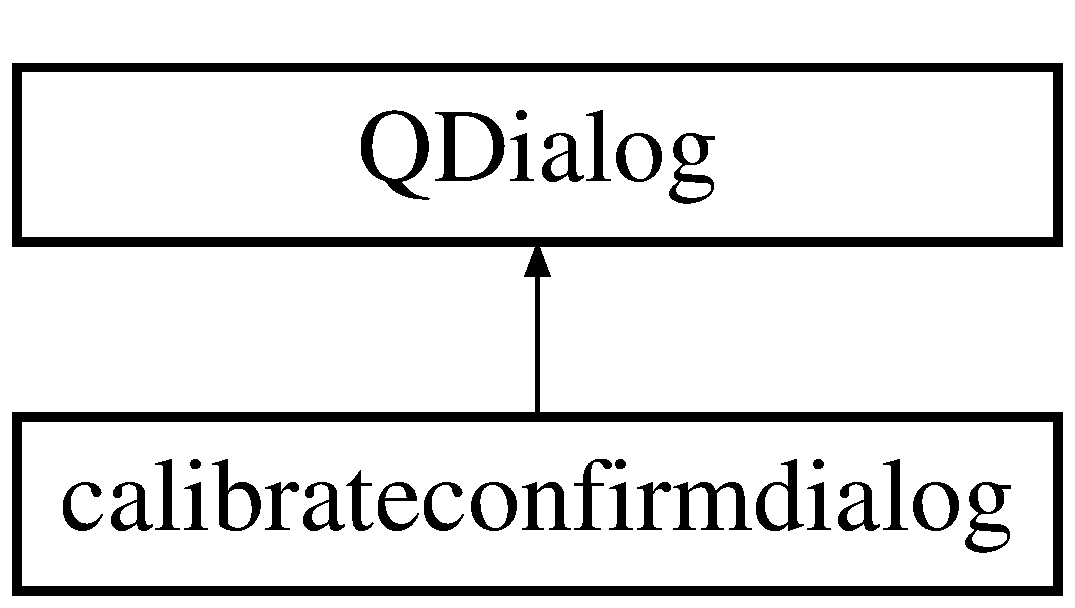
\includegraphics[height=2.000000cm]{classcalibrateconfirmdialog}
\end{center}
\end{figure}
\subsection*{Public Slots}
\begin{DoxyCompactItemize}
\item 
\hypertarget{classcalibrateconfirmdialog_a8579c47f6d8634ddb6acde470894aa7d}{}void {\bfseries update\+Left\+Progress} (int number\+\_\+done)\label{classcalibrateconfirmdialog_a8579c47f6d8634ddb6acde470894aa7d}

\item 
\hypertarget{classcalibrateconfirmdialog_a1f5748596aa11125e1ce010df142aa2c}{}void {\bfseries update\+Right\+Progress} (int number\+\_\+done)\label{classcalibrateconfirmdialog_a1f5748596aa11125e1ce010df142aa2c}

\end{DoxyCompactItemize}
\subsection*{Public Member Functions}
\begin{DoxyCompactItemize}
\item 
\hypertarget{classcalibrateconfirmdialog_ad441884efbb852e887fbd1e76e23655d}{}{\bfseries calibrateconfirmdialog} (Q\+Widget $\ast$parent=0)\label{classcalibrateconfirmdialog_ad441884efbb852e887fbd1e76e23655d}

\item 
\hypertarget{classcalibrateconfirmdialog_a1ff7049a8a9fd467ab524fa29034ce5f}{}void {\bfseries update\+Left} (const cv\+::\+Mat \&camera\+\_\+matrix, const cv\+::\+Mat \&distortion, const double \&rms)\label{classcalibrateconfirmdialog_a1ff7049a8a9fd467ab524fa29034ce5f}

\item 
\hypertarget{classcalibrateconfirmdialog_a8bd5859b51d6196ee042e7c6212a3a37}{}void {\bfseries update\+Right} (const cv\+::\+Mat \&camera\+\_\+matrix, const cv\+::\+Mat \&distortion, const double \&rms)\label{classcalibrateconfirmdialog_a8bd5859b51d6196ee042e7c6212a3a37}

\item 
\hypertarget{classcalibrateconfirmdialog_a57e87da51c71e7e247520ae53ff3ac4f}{}void {\bfseries update\+Stereo} (const cv\+::\+Mat Q, const double \&rms)\label{classcalibrateconfirmdialog_a57e87da51c71e7e247520ae53ff3ac4f}

\item 
\hypertarget{classcalibrateconfirmdialog_ab5482a638c5af7c0d1a6ebfb57972d76}{}void {\bfseries set\+Number\+Images} (int number\+\_\+images)\label{classcalibrateconfirmdialog_ab5482a638c5af7c0d1a6ebfb57972d76}

\end{DoxyCompactItemize}


\subsection{Detailed Description}


Definition at line 16 of file calibrateconfirmdialog.\+h.



The documentation for this class was generated from the following files\+:\begin{DoxyCompactItemize}
\item 
src/calibrateconfirmdialog.\+h\item 
src/calibrateconfirmdialog.\+cpp\end{DoxyCompactItemize}

\hypertarget{class_calibrate_from_images_dialog}{}\section{Calibrate\+From\+Images\+Dialog Class Reference}
\label{class_calibrate_from_images_dialog}\index{Calibrate\+From\+Images\+Dialog@{Calibrate\+From\+Images\+Dialog}}
Inheritance diagram for Calibrate\+From\+Images\+Dialog\+:\begin{figure}[H]
\begin{center}
\leavevmode
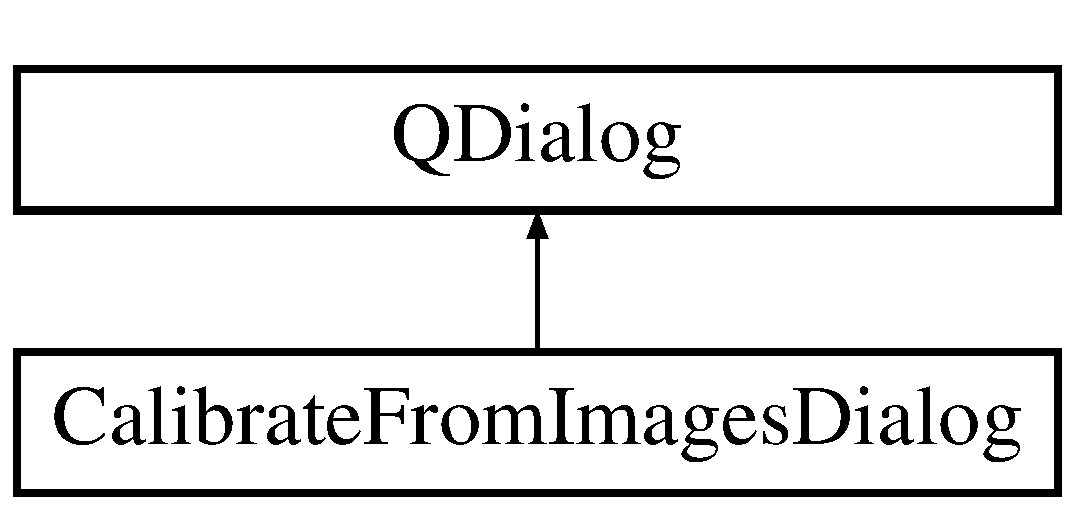
\includegraphics[height=2.000000cm]{class_calibrate_from_images_dialog}
\end{center}
\end{figure}
\subsection*{Signals}
\begin{DoxyCompactItemize}
\item 
\hypertarget{class_calibrate_from_images_dialog_a1733440fa386d1482cbf7dc2704c2612}{}void {\bfseries run\+\_\+calibration} ()\label{class_calibrate_from_images_dialog_a1733440fa386d1482cbf7dc2704c2612}

\end{DoxyCompactItemize}
\subsection*{Public Member Functions}
\begin{DoxyCompactItemize}
\item 
\hypertarget{class_calibrate_from_images_dialog_afe59dd44c63c22043a93c37bff3c8d57}{}{\bfseries Calibrate\+From\+Images\+Dialog} (Q\+Widget $\ast$parent=0)\label{class_calibrate_from_images_dialog_afe59dd44c63c22043a93c37bff3c8d57}

\item 
\hypertarget{class_calibrate_from_images_dialog_ad5f15a31b9ca81caf82709ebae582adf}{}Q\+List$<$ Q\+String $>$ {\bfseries get\+Left\+Images} ()\label{class_calibrate_from_images_dialog_ad5f15a31b9ca81caf82709ebae582adf}

\item 
\hypertarget{class_calibrate_from_images_dialog_a475cc42908143419572a8c170f2771f2}{}Q\+List$<$ Q\+String $>$ {\bfseries get\+Right\+Images} ()\label{class_calibrate_from_images_dialog_a475cc42908143419572a8c170f2771f2}

\item 
\hypertarget{class_calibrate_from_images_dialog_ae59e54f4d5b5e70ab518ba7aa39d8c0a}{}int {\bfseries get\+Pattern\+Cols} ()\label{class_calibrate_from_images_dialog_ae59e54f4d5b5e70ab518ba7aa39d8c0a}

\item 
\hypertarget{class_calibrate_from_images_dialog_a34af5e3a9537cfe4785c4f24c6a3460d}{}int {\bfseries get\+Pattern\+Rows} ()\label{class_calibrate_from_images_dialog_a34af5e3a9537cfe4785c4f24c6a3460d}

\item 
\hypertarget{class_calibrate_from_images_dialog_a52c6ef5e5e32a815fcc424182fb97607}{}double {\bfseries get\+Square\+Size\+Mm} ()\label{class_calibrate_from_images_dialog_a52c6ef5e5e32a815fcc424182fb97607}

\end{DoxyCompactItemize}


\subsection{Detailed Description}


Definition at line 26 of file calibratefromimagesdialog.\+h.



The documentation for this class was generated from the following files\+:\begin{DoxyCompactItemize}
\item 
src/calibratefromimagesdialog.\+h\item 
src/calibratefromimagesdialog.\+cpp\end{DoxyCompactItemize}

\hypertarget{class_calibration_dialog}{}\section{Calibration\+Dialog Class Reference}
\label{class_calibration_dialog}\index{Calibration\+Dialog@{Calibration\+Dialog}}
Inheritance diagram for Calibration\+Dialog\+:\begin{figure}[H]
\begin{center}
\leavevmode
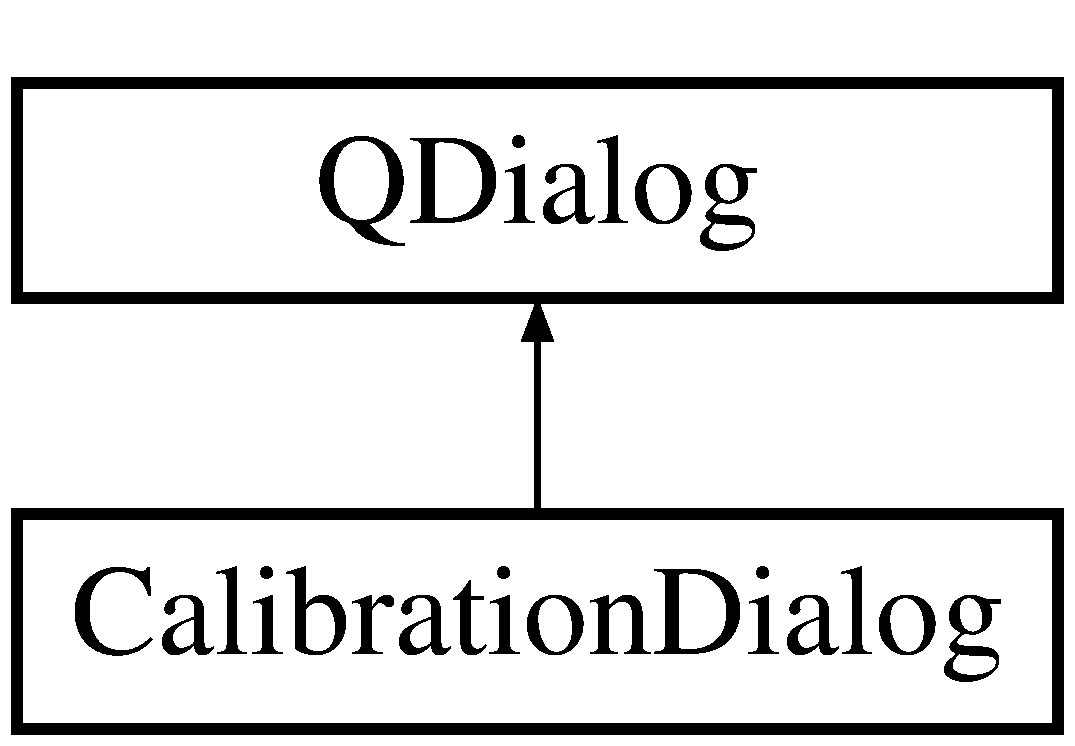
\includegraphics[height=2.000000cm]{class_calibration_dialog}
\end{center}
\end{figure}
\subsection*{Public Slots}
\begin{DoxyCompactItemize}
\item 
\hypertarget{class_calibration_dialog_aa93f4f8df0d73fe6a9c005ee0fe6bb24}{}void {\bfseries set\+Image\+Progress} (int current, int total)\label{class_calibration_dialog_aa93f4f8df0d73fe6a9c005ee0fe6bb24}

\item 
\hypertarget{class_calibration_dialog_a7325731e673238cdaa9c8292fc8188e9}{}void {\bfseries update\+Labels} (\hyperlink{class_chessboard}{Chessboard} $\ast$board)\label{class_calibration_dialog_a7325731e673238cdaa9c8292fc8188e9}

\end{DoxyCompactItemize}
\subsection*{Signals}
\begin{DoxyCompactItemize}
\item 
\hypertarget{class_calibration_dialog_a0dbbfdbd304e257105e807fc40d494cf}{}void {\bfseries stop\+Calibration} ()\label{class_calibration_dialog_a0dbbfdbd304e257105e807fc40d494cf}

\end{DoxyCompactItemize}
\subsection*{Public Member Functions}
\begin{DoxyCompactItemize}
\item 
\hypertarget{class_calibration_dialog_aacf17330c3788d302c7e83fd2e9dbef6}{}{\bfseries Calibration\+Dialog} (Q\+Widget $\ast$parent=0, \hyperlink{class_stereo_calibrate}{Stereo\+Calibrate} $\ast$calibrator=0)\label{class_calibration_dialog_aacf17330c3788d302c7e83fd2e9dbef6}

\end{DoxyCompactItemize}


\subsection{Detailed Description}


Definition at line 18 of file calibrationdialog.\+h.



The documentation for this class was generated from the following files\+:\begin{DoxyCompactItemize}
\item 
src/calibrationdialog.\+h\item 
src/calibrationdialog.\+cpp\end{DoxyCompactItemize}

\hypertarget{class_camera_open_c_v}{}\section{Camera\+Open\+C\+V Class Reference}
\label{class_camera_open_c_v}\index{Camera\+Open\+C\+V@{Camera\+Open\+C\+V}}
Inheritance diagram for Camera\+Open\+C\+V\+:\begin{figure}[H]
\begin{center}
\leavevmode
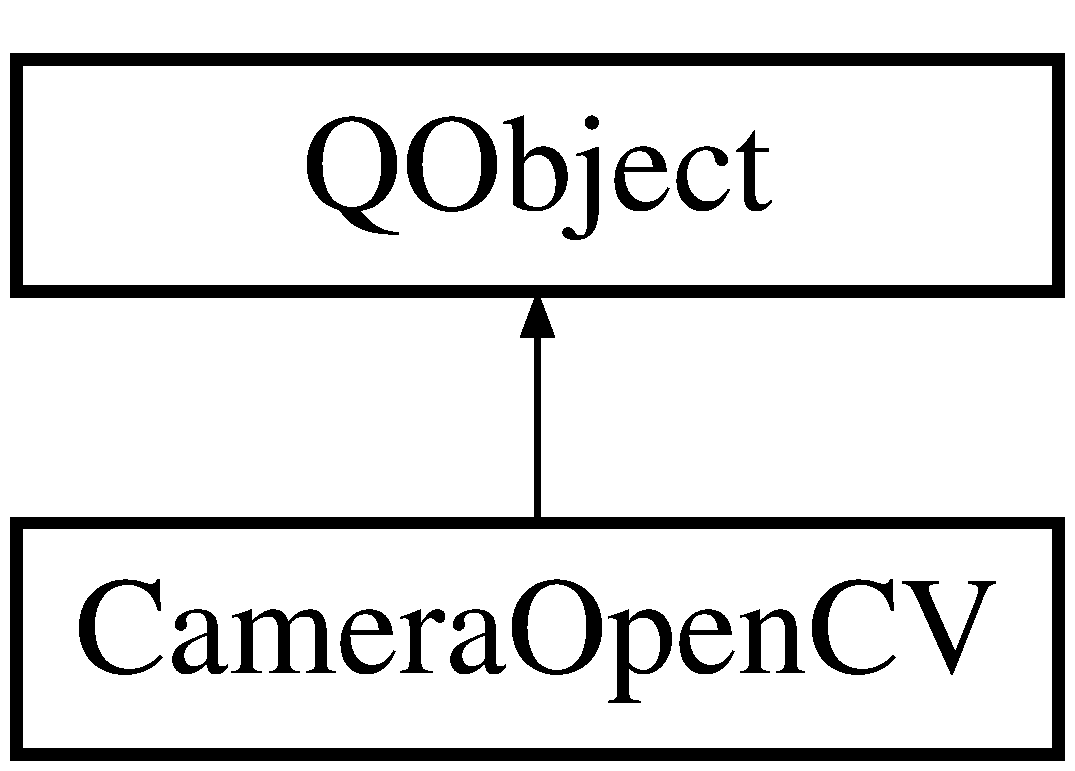
\includegraphics[height=2.000000cm]{class_camera_open_c_v}
\end{center}
\end{figure}
\subsection*{Public Slots}
\begin{DoxyCompactItemize}
\item 
\hypertarget{class_camera_open_c_v_ac3835c145a33eb30d52fe11c3a226aef}{}bool {\bfseries capture} (void)\label{class_camera_open_c_v_ac3835c145a33eb30d52fe11c3a226aef}

\item 
\hypertarget{class_camera_open_c_v_a319723113eebfc9f844176fc40d03429}{}cv\+::\+Mat $\ast$ {\bfseries get\+Image} (void)\label{class_camera_open_c_v_a319723113eebfc9f844176fc40d03429}

\end{DoxyCompactItemize}
\subsection*{Signals}
\begin{DoxyCompactItemize}
\item 
\hypertarget{class_camera_open_c_v_a5efd166aa1423d798dc501a31da0cdec}{}void {\bfseries captured} ()\label{class_camera_open_c_v_a5efd166aa1423d798dc501a31da0cdec}

\item 
\hypertarget{class_camera_open_c_v_ab71fb7050b5a1b42eae2239100612bd3}{}void {\bfseries finished} ()\label{class_camera_open_c_v_ab71fb7050b5a1b42eae2239100612bd3}

\end{DoxyCompactItemize}
\subsection*{Public Member Functions}
\begin{DoxyCompactItemize}
\item 
\hypertarget{class_camera_open_c_v_a11513f82fb6525837b669a1f577a4b4c}{}{\bfseries Camera\+Open\+C\+V} (Q\+Object $\ast$parent=0)\label{class_camera_open_c_v_a11513f82fb6525837b669a1f577a4b4c}

\item 
\hypertarget{class_camera_open_c_v_a4f74abae529642b30ed20e7edd34f242}{}bool {\bfseries is\+Available} ()\label{class_camera_open_c_v_a4f74abae529642b30ed20e7edd34f242}

\item 
\hypertarget{class_camera_open_c_v_af0aaccf4308f82ce69f9291734145b0f}{}void {\bfseries close} ()\label{class_camera_open_c_v_af0aaccf4308f82ce69f9291734145b0f}

\item 
\hypertarget{class_camera_open_c_v_a85716a1a309bf8269d3767002989c126}{}bool {\bfseries init\+Camera} (int index)\label{class_camera_open_c_v_a85716a1a309bf8269d3767002989c126}

\item 
\hypertarget{class_camera_open_c_v_a2790e5210b7dc3a4b096e95458c6264a}{}void {\bfseries assign\+Thread} (Q\+Thread $\ast$thread)\label{class_camera_open_c_v_a2790e5210b7dc3a4b096e95458c6264a}

\item 
\hypertarget{class_camera_open_c_v_a7b63193973da529de09142fffac0555e}{}void {\bfseries get\+Image\+Size} (int \&image\+\_\+width, int \&image\+\_\+height, cv\+::\+Size \&image\+\_\+size)\label{class_camera_open_c_v_a7b63193973da529de09142fffac0555e}

\item 
\hypertarget{class_camera_open_c_v_ab79a0b312192ae4a76aee9019271b4c0}{}bool {\bfseries set\+Frame16} ()\label{class_camera_open_c_v_ab79a0b312192ae4a76aee9019271b4c0}

\item 
\hypertarget{class_camera_open_c_v_a919ff5c55965b8d27ebb3e092398873f}{}bool {\bfseries set\+Frame8} ()\label{class_camera_open_c_v_a919ff5c55965b8d27ebb3e092398873f}

\item 
\hypertarget{class_camera_open_c_v_af090db8f2a6edfaece533b2fdbbd9a21}{}bool {\bfseries set\+Maximum\+Resolution} ()\label{class_camera_open_c_v_af090db8f2a6edfaece533b2fdbbd9a21}

\item 
\hypertarget{class_camera_open_c_v_a1214731f8a3bd3cfbc11a065bc93c806}{}bool {\bfseries set\+Exposure} (double exposure)\label{class_camera_open_c_v_a1214731f8a3bd3cfbc11a065bc93c806}

\item 
\hypertarget{class_camera_open_c_v_af1a30a1dda23ba15ffc4feb41718e7e6}{}bool {\bfseries set\+Gain} (double gain)\label{class_camera_open_c_v_af1a30a1dda23ba15ffc4feb41718e7e6}

\end{DoxyCompactItemize}


\subsection{Detailed Description}


Definition at line 15 of file cameraopencv.\+h.



The documentation for this class was generated from the following files\+:\begin{DoxyCompactItemize}
\item 
src/cameraopencv.\+h\item 
src/cameraopencv.\+cpp\end{DoxyCompactItemize}

\hypertarget{class_chessboard}{}\section{Chessboard Class Reference}
\label{class_chessboard}\index{Chessboard@{Chessboard}}
Inheritance diagram for Chessboard\+:\begin{figure}[H]
\begin{center}
\leavevmode
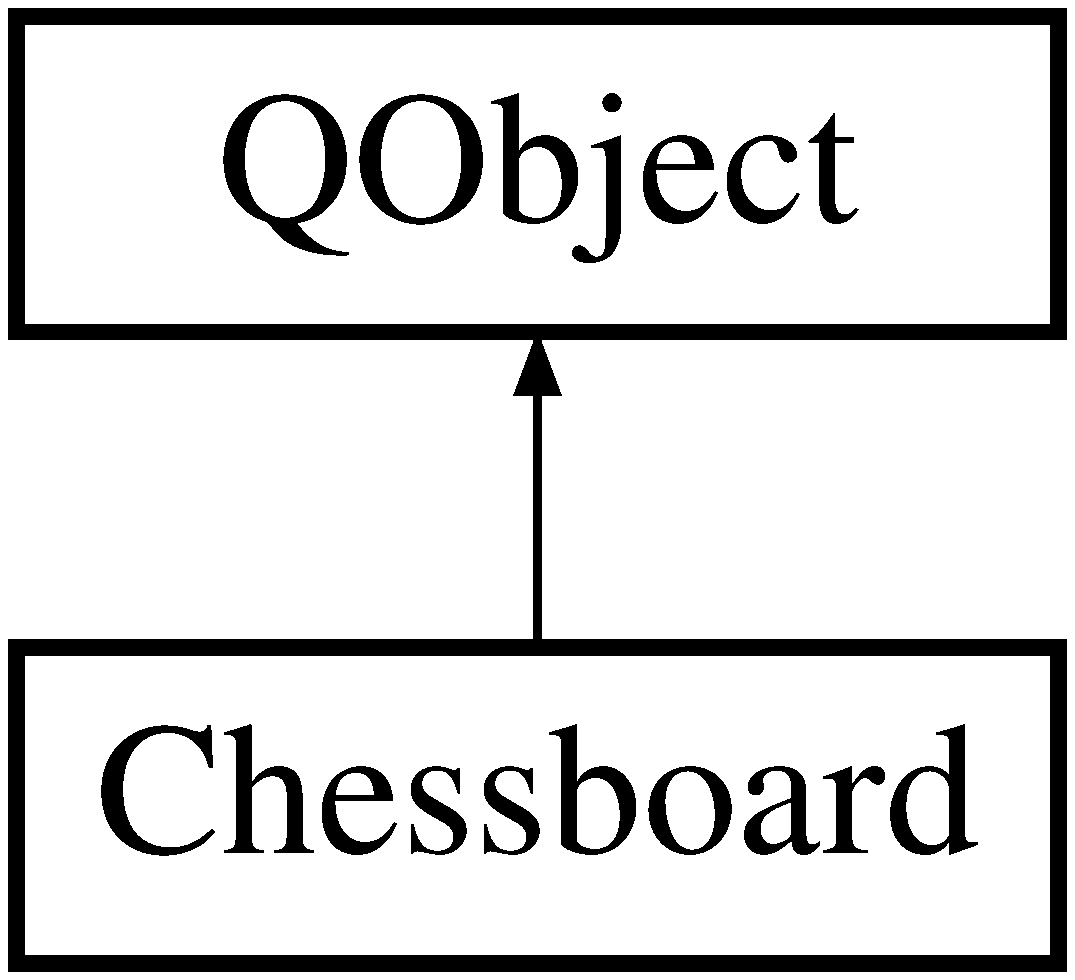
\includegraphics[height=2.000000cm]{class_chessboard}
\end{center}
\end{figure}
\subsection*{Public Slots}
\begin{DoxyCompactItemize}
\item 
\hypertarget{class_chessboard_a8fbbd9febc14f3ae267b7d604a707881}{}void {\bfseries set\+Horizontal\+Tilt} (double min\+\_\+horizontal\+\_\+tilt, double max\+\_\+horizontal\+\_\+tilt)\label{class_chessboard_a8fbbd9febc14f3ae267b7d604a707881}

\item 
\hypertarget{class_chessboard_a24bdb477cbcfbc5c4c8c12bfd1071766}{}void {\bfseries set\+Vertical\+Tilt} (double min\+\_\+vertical\+\_\+tilt, double max\+\_\+vertical\+\_\+tilt)\label{class_chessboard_a24bdb477cbcfbc5c4c8c12bfd1071766}

\item 
\hypertarget{class_chessboard_a5a12f6cf4a21d747cfb3750138a45d4f}{}void {\bfseries set\+Board\+Area} (double min\+\_\+area, double max\+\_\+area)\label{class_chessboard_a5a12f6cf4a21d747cfb3750138a45d4f}

\item 
\hypertarget{class_chessboard_afa4754bf5a642a988299484ec15c1866}{}void {\bfseries set\+Board\+Margins} (double left\+\_\+margin, double right\+\_\+margin, double top\+\_\+margin, double bottom\+\_\+margin)\label{class_chessboard_afa4754bf5a642a988299484ec15c1866}

\item 
\hypertarget{class_chessboard_ae0e3fed17637712166ababe977e88ae5}{}bool {\bfseries check} (std\+::vector$<$ cv\+::\+Point2f $>$ \&board\+\_\+points)\label{class_chessboard_ae0e3fed17637712166ababe977e88ae5}

\item 
\hypertarget{class_chessboard_a9fed083db7f8b8576730d80131d5b506}{}bool {\bfseries is\+Valid} (void)\label{class_chessboard_a9fed083db7f8b8576730d80131d5b506}

\end{DoxyCompactItemize}
\subsection*{Signals}
\begin{DoxyCompactItemize}
\item 
\hypertarget{class_chessboard_a9daceb67cea253e4178cf353f55a973b}{}void {\bfseries got\+Tilts} (double horizontal, double vertical)\label{class_chessboard_a9daceb67cea253e4178cf353f55a973b}

\item 
\hypertarget{class_chessboard_a98bac12fdee79933052af01a501a3735}{}void {\bfseries got\+Area} (double area)\label{class_chessboard_a98bac12fdee79933052af01a501a3735}

\end{DoxyCompactItemize}
\subsection*{Public Member Functions}
\begin{DoxyCompactItemize}
\item 
\hypertarget{class_chessboard_a422d312bd00059b1c3947276dbd8a765}{}{\bfseries Chessboard} (Q\+Object $\ast$parent=0, cv\+::\+Size pattern=cv\+::\+Size(0, 0), cv\+::\+Size imsize=cv\+::\+Size(0, 0))\label{class_chessboard_a422d312bd00059b1c3947276dbd8a765}

\item 
\hypertarget{class_chessboard_af0c13ce21b47526dad57770bfd3ea744}{}void {\bfseries set\+Template} (std\+::vector$<$ cv\+::\+Point2i $>$ contour)\label{class_chessboard_af0c13ce21b47526dad57770bfd3ea744}

\item 
\hypertarget{class_chessboard_aedcbee8b6cb47587b4b68051611400e9}{}bool {\bfseries check\+Against\+Template} ()\label{class_chessboard_aedcbee8b6cb47587b4b68051611400e9}

\item 
\hypertarget{class_chessboard_ac7c8d73a26dcab8af62bc484f46e2057}{}double {\bfseries get\+Area} ()\label{class_chessboard_ac7c8d73a26dcab8af62bc484f46e2057}

\end{DoxyCompactItemize}
\subsection*{Public Attributes}
\begin{DoxyCompactItemize}
\item 
\hypertarget{class_chessboard_a1b09ada63972bbb716c9f0681e0d3453}{}double {\bfseries min\+\_\+horizontal\+\_\+tilt} = -\/0.\+1\label{class_chessboard_a1b09ada63972bbb716c9f0681e0d3453}

\item 
\hypertarget{class_chessboard_a64f1c36828343944eef1aa978c0875c8}{}double {\bfseries max\+\_\+horizontal\+\_\+tilt} = 0.\+1\label{class_chessboard_a64f1c36828343944eef1aa978c0875c8}

\item 
\hypertarget{class_chessboard_a938a6ea0cd5fcbe19aff7e761d9a5acf}{}double {\bfseries min\+\_\+vertical\+\_\+tilt} = -\/0.\+1\label{class_chessboard_a938a6ea0cd5fcbe19aff7e761d9a5acf}

\item 
\hypertarget{class_chessboard_aec73a4e87cc92d0eed59b3a01cab2045}{}double {\bfseries max\+\_\+vertical\+\_\+tilt} = 0.\+1\label{class_chessboard_aec73a4e87cc92d0eed59b3a01cab2045}

\item 
\hypertarget{class_chessboard_a61a98c08d7afed4cc2a811c939f94c1d}{}double {\bfseries min\+\_\+area} = 0.\+4\label{class_chessboard_a61a98c08d7afed4cc2a811c939f94c1d}

\item 
\hypertarget{class_chessboard_ad923d38e1ffe977f74b39a740372f388}{}double {\bfseries max\+\_\+area} = 1\label{class_chessboard_ad923d38e1ffe977f74b39a740372f388}

\item 
\hypertarget{class_chessboard_ac4181368e11b6b8ad2d4c24f123f947a}{}double {\bfseries left\+\_\+margin} = -\/1\label{class_chessboard_ac4181368e11b6b8ad2d4c24f123f947a}

\item 
\hypertarget{class_chessboard_a17bafedcdfd05f9fd7cd7b66d2bfd332}{}double {\bfseries right\+\_\+margin} = -\/1\label{class_chessboard_a17bafedcdfd05f9fd7cd7b66d2bfd332}

\item 
\hypertarget{class_chessboard_ad608ddf2389a901a33955c223f804dce}{}double {\bfseries top\+\_\+margin} = -\/1\label{class_chessboard_ad608ddf2389a901a33955c223f804dce}

\item 
\hypertarget{class_chessboard_a6d5d78943038a610f856bf1d0a75f118}{}double {\bfseries bottom\+\_\+margin} = -\/1\label{class_chessboard_a6d5d78943038a610f856bf1d0a75f118}

\item 
\hypertarget{class_chessboard_a92dee8c30ad43afac1031e31d4bba522}{}bool {\bfseries valid} = false\label{class_chessboard_a92dee8c30ad43afac1031e31d4bba522}

\item 
\hypertarget{class_chessboard_af5216c30e0da8a4949264bf6533303d8}{}double {\bfseries horizontal\+\_\+tilt}\label{class_chessboard_af5216c30e0da8a4949264bf6533303d8}

\item 
\hypertarget{class_chessboard_a4923208e2c20af7fbb090b0716b03b72}{}double {\bfseries vertical\+\_\+tilt}\label{class_chessboard_a4923208e2c20af7fbb090b0716b03b72}

\item 
\hypertarget{class_chessboard_a54249eb30bfd3057137ba1f5357c47a5}{}double {\bfseries left\+\_\+length}\label{class_chessboard_a54249eb30bfd3057137ba1f5357c47a5}

\item 
\hypertarget{class_chessboard_a658739d7b80175ce6cf737b61197f977}{}double {\bfseries right\+\_\+length}\label{class_chessboard_a658739d7b80175ce6cf737b61197f977}

\item 
\hypertarget{class_chessboard_a0242965da64a1fedc1f97df17f4f337c}{}double {\bfseries top\+\_\+length}\label{class_chessboard_a0242965da64a1fedc1f97df17f4f337c}

\item 
\hypertarget{class_chessboard_a90bd093500d7a5f6a8f705f12f9a9028}{}double {\bfseries bottom\+\_\+length}\label{class_chessboard_a90bd093500d7a5f6a8f705f12f9a9028}

\item 
\hypertarget{class_chessboard_a34aad177677a2dc5b70ab6754b8ec67b}{}bool {\bfseries left\+\_\+out\+\_\+of\+\_\+bounds} = true\label{class_chessboard_a34aad177677a2dc5b70ab6754b8ec67b}

\item 
\hypertarget{class_chessboard_ac2cac094775d118dc15287e2352c90a4}{}bool {\bfseries right\+\_\+out\+\_\+of\+\_\+bounds} = true\label{class_chessboard_ac2cac094775d118dc15287e2352c90a4}

\item 
\hypertarget{class_chessboard_abf013ccb0d2b98d34d75ed41dba14452}{}bool {\bfseries top\+\_\+out\+\_\+of\+\_\+bounds} = true\label{class_chessboard_abf013ccb0d2b98d34d75ed41dba14452}

\item 
\hypertarget{class_chessboard_aa15fcba3656e38be25ffa3507f6bb4ee}{}bool {\bfseries bottom\+\_\+out\+\_\+of\+\_\+bounds} = true\label{class_chessboard_aa15fcba3656e38be25ffa3507f6bb4ee}

\item 
\hypertarget{class_chessboard_a71743d34a3b481920b12911d124e4f8f}{}bool {\bfseries horizontal\+\_\+tilt\+\_\+under} = true\label{class_chessboard_a71743d34a3b481920b12911d124e4f8f}

\item 
\hypertarget{class_chessboard_aeeffb94596579ff45f1ca7015cb724c9}{}bool {\bfseries horizontal\+\_\+tilt\+\_\+over} = true\label{class_chessboard_aeeffb94596579ff45f1ca7015cb724c9}

\item 
\hypertarget{class_chessboard_a4a645e50f7b3f40f381854abbf2f45ab}{}bool {\bfseries vertical\+\_\+tilt\+\_\+under} = true\label{class_chessboard_a4a645e50f7b3f40f381854abbf2f45ab}

\item 
\hypertarget{class_chessboard_a362fcb984a0a7dd0f90d4d12ed71a3ea}{}bool {\bfseries vertical\+\_\+tilt\+\_\+over} = true\label{class_chessboard_a362fcb984a0a7dd0f90d4d12ed71a3ea}

\item 
\hypertarget{class_chessboard_ab81ab95920e11957774d0d831299fe5f}{}bool {\bfseries board\+\_\+area\+\_\+under}\label{class_chessboard_ab81ab95920e11957774d0d831299fe5f}

\item 
\hypertarget{class_chessboard_af1948e8b9d45efc716295808d7aa6ee0}{}bool {\bfseries board\+\_\+area\+\_\+over}\label{class_chessboard_af1948e8b9d45efc716295808d7aa6ee0}

\item 
\hypertarget{class_chessboard_aff5056bb3510926b3d5e896bdbed00a3}{}std\+::vector$<$ cv\+::\+Point2f $>$ {\bfseries board\+\_\+points}\label{class_chessboard_aff5056bb3510926b3d5e896bdbed00a3}

\item 
\hypertarget{class_chessboard_a218855537ee771c0ad557ff8142bb5c9}{}std\+::vector$<$ cv\+::\+Point2f $>$ {\bfseries top\+\_\+points}\label{class_chessboard_a218855537ee771c0ad557ff8142bb5c9}

\item 
\hypertarget{class_chessboard_a9c38d739b272a46321be0d2eea58b8b8}{}std\+::vector$<$ cv\+::\+Point2f $>$ {\bfseries left\+\_\+points}\label{class_chessboard_a9c38d739b272a46321be0d2eea58b8b8}

\item 
\hypertarget{class_chessboard_a877d70697b755622bdf9b0e1ad5c441e}{}std\+::vector$<$ cv\+::\+Point2f $>$ {\bfseries right\+\_\+points}\label{class_chessboard_a877d70697b755622bdf9b0e1ad5c441e}

\item 
\hypertarget{class_chessboard_a601ac1447dcdb89692f1eaad2f217786}{}std\+::vector$<$ cv\+::\+Point2f $>$ {\bfseries bottom\+\_\+points}\label{class_chessboard_a601ac1447dcdb89692f1eaad2f217786}

\item 
\hypertarget{class_chessboard_a463faa4bf94ddbc54358eb01634920ca}{}std\+::vector$<$ cv\+::\+Point2f $>$ {\bfseries vertices}\label{class_chessboard_a463faa4bf94ddbc54358eb01634920ca}

\item 
\hypertarget{class_chessboard_a8aaff50d8e307ba8a6ce7a1e04095d57}{}std\+::vector$<$ cv\+::\+Point2i $>$ {\bfseries template\+\_\+contour}\label{class_chessboard_a8aaff50d8e307ba8a6ce7a1e04095d57}

\end{DoxyCompactItemize}


\subsection{Detailed Description}


Definition at line 13 of file chessboard.\+h.



The documentation for this class was generated from the following files\+:\begin{DoxyCompactItemize}
\item 
src/chessboard.\+h\item 
src/chessboard.\+cpp\end{DoxyCompactItemize}

\hypertarget{class_disparity_viewer}{}\section{Disparity\+Viewer Class Reference}
\label{class_disparity_viewer}\index{Disparity\+Viewer@{Disparity\+Viewer}}
Inheritance diagram for Disparity\+Viewer\+:\begin{figure}[H]
\begin{center}
\leavevmode
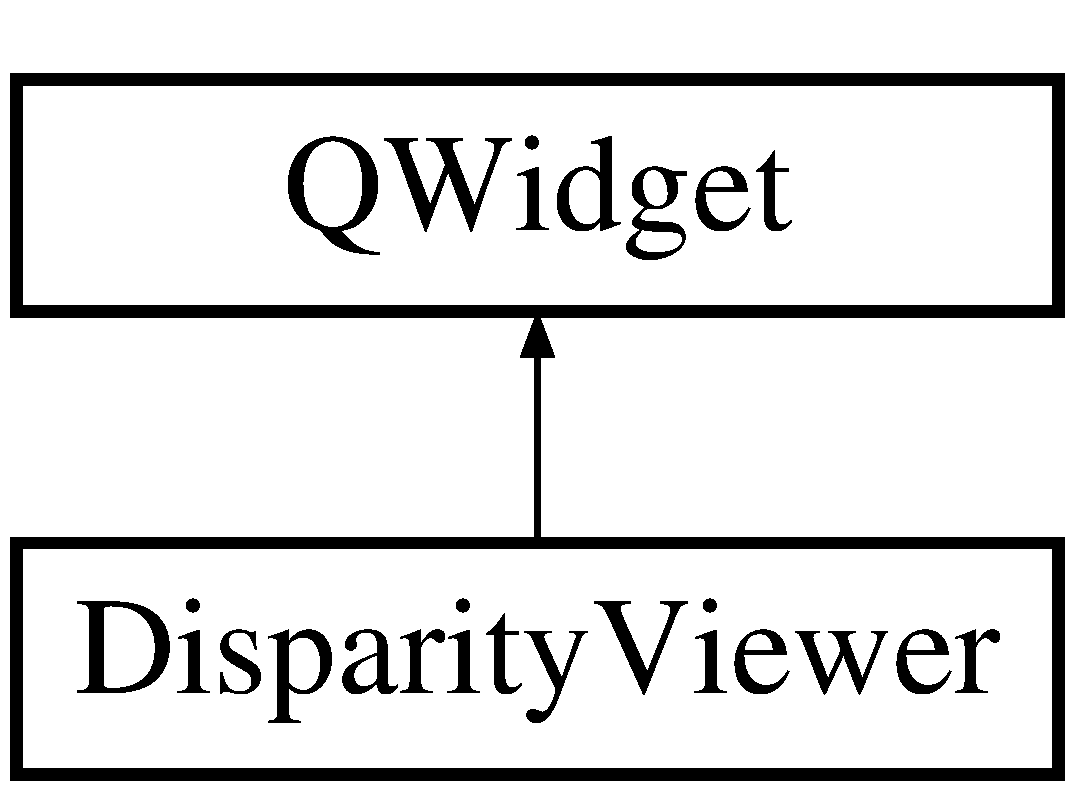
\includegraphics[height=2.000000cm]{class_disparity_viewer}
\end{center}
\end{figure}
\subsection*{Public Slots}
\begin{DoxyCompactItemize}
\item 
\hypertarget{class_disparity_viewer_a2ed25874b1180e197fea72c1281750a6}{}void {\bfseries update\+Disparity} (void)\label{class_disparity_viewer_a2ed25874b1180e197fea72c1281750a6}

\item 
\hypertarget{class_disparity_viewer_a988ce413da8823c64bf190dfc359f16f}{}void {\bfseries update\+Disparity\+Async} (void)\label{class_disparity_viewer_a988ce413da8823c64bf190dfc359f16f}

\item 
\hypertarget{class_disparity_viewer_a75a907708436c6805b6318eb90d96369}{}void {\bfseries set\+Matcher} (\hyperlink{class_abstract_stereo_matcher}{Abstract\+Stereo\+Matcher} $\ast$matcher)\label{class_disparity_viewer_a75a907708436c6805b6318eb90d96369}

\item 
\hypertarget{class_disparity_viewer_a5d060a1bd1867db8938f6247e1bbdc2c}{}void {\bfseries set\+Colourmap} (int)\label{class_disparity_viewer_a5d060a1bd1867db8938f6247e1bbdc2c}

\item 
\hypertarget{class_disparity_viewer_ab4dd876b0a61d2bd7ad3054cf1b86b38}{}void {\bfseries set\+Calibration} (cv\+::\+Mat \&Q, double baseline=1.\+0, double focal=1.\+0)\label{class_disparity_viewer_ab4dd876b0a61d2bd7ad3054cf1b86b38}

\item 
\hypertarget{class_disparity_viewer_a7f12cd7a395428fe6819ae29cec31a5d}{}void {\bfseries update\+Pixmap\+Range} ()\label{class_disparity_viewer_a7f12cd7a395428fe6819ae29cec31a5d}

\end{DoxyCompactItemize}
\subsection*{Signals}
\begin{DoxyCompactItemize}
\item 
\hypertarget{class_disparity_viewer_ac1f50ec04e6fcaa0b8a7cbb214f9c148}{}void {\bfseries finished} ()\label{class_disparity_viewer_ac1f50ec04e6fcaa0b8a7cbb214f9c148}

\item 
\hypertarget{class_disparity_viewer_afd82a842f154a3ae24090048476f49eb}{}void {\bfseries new\+Disparity} (Q\+Pixmap)\label{class_disparity_viewer_afd82a842f154a3ae24090048476f49eb}

\end{DoxyCompactItemize}
\subsection*{Public Member Functions}
\begin{DoxyCompactItemize}
\item 
\hypertarget{class_disparity_viewer_ad373b498801c6bdc3e2d6835a60e8611}{}{\bfseries Disparity\+Viewer} (Q\+Widget $\ast$parent=0)\label{class_disparity_viewer_ad373b498801c6bdc3e2d6835a60e8611}

\item 
\hypertarget{class_disparity_viewer_a7224a0cc574ec3b7255edc35ee80094b}{}void {\bfseries set\+Viewer} (Q\+Label $\ast$viewer)\label{class_disparity_viewer_a7224a0cc574ec3b7255edc35ee80094b}

\item 
\hypertarget{class_disparity_viewer_a67aec5bc6a1c7160f997b29f1e486d40}{}void {\bfseries assign\+Thread} (Q\+Thread $\ast$thread)\label{class_disparity_viewer_a67aec5bc6a1c7160f997b29f1e486d40}

\end{DoxyCompactItemize}


\subsection{Detailed Description}


Definition at line 20 of file disparityviewer.\+h.



The documentation for this class was generated from the following files\+:\begin{DoxyCompactItemize}
\item 
src/disparityviewer.\+h\item 
src/disparityviewer.\+cpp\end{DoxyCompactItemize}

\hypertarget{class_main_window}{}\section{Main\+Window Class Reference}
\label{class_main_window}\index{Main\+Window@{Main\+Window}}
Inheritance diagram for Main\+Window\+:\begin{figure}[H]
\begin{center}
\leavevmode
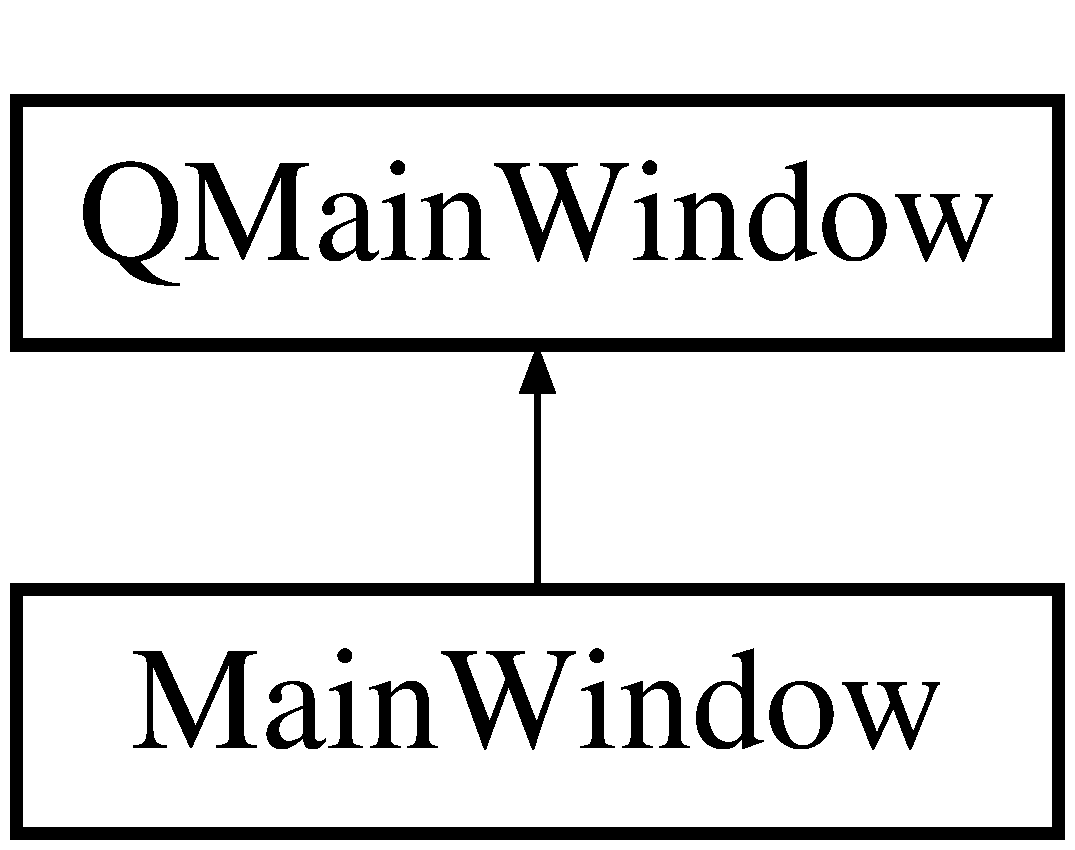
\includegraphics[height=2.000000cm]{class_main_window}
\end{center}
\end{figure}
\subsection*{Public Slots}
\begin{DoxyCompactItemize}
\item 
\hypertarget{class_main_window_a868f3d9f348391b74184bc94dcc118e3}{}void {\bfseries update\+Display} (void)\label{class_main_window_a868f3d9f348391b74184bc94dcc118e3}

\item 
\hypertarget{class_main_window_a56ebe4326012743d86f097d2338480f8}{}void {\bfseries update\+F\+P\+S} (qint64)\label{class_main_window_a56ebe4326012743d86f097d2338480f8}

\item 
\hypertarget{class_main_window_a1b4b4a8946e42e552dd750017d531fd1}{}void {\bfseries update\+Temperature} (double temperature)\label{class_main_window_a1b4b4a8946e42e552dd750017d531fd1}

\item 
\hypertarget{class_main_window_aa2b38963b399e878dc42f9533a41573f}{}void {\bfseries update\+Frame\+Count} (qint64)\label{class_main_window_aa2b38963b399e878dc42f9533a41573f}

\item 
\hypertarget{class_main_window_a05ff6c00dc738e54a284e22d11d982e9}{}void {\bfseries toggle\+Acquire} (void)\label{class_main_window_a05ff6c00dc738e54a284e22d11d982e9}

\item 
\hypertarget{class_main_window_a471dce2a5fbc004c344d7207e7aa8b3e}{}void {\bfseries single\+Shot\+Clicked} (void)\label{class_main_window_a471dce2a5fbc004c344d7207e7aa8b3e}

\item 
\hypertarget{class_main_window_af0c7c203e4f8d0b953c7c94d7724d8b2}{}void {\bfseries save\+Single} (void)\label{class_main_window_af0c7c203e4f8d0b953c7c94d7724d8b2}

\item 
\hypertarget{class_main_window_a5c4947f5e5a4b2e305ea4445873e162f}{}void {\bfseries display\+Saved} (Q\+String fname)\label{class_main_window_a5c4947f5e5a4b2e305ea4445873e162f}

\item 
\hypertarget{class_main_window_ae58c31493b548d8de907b152596f459e}{}void {\bfseries status\+Message\+Timeout} (void)\label{class_main_window_ae58c31493b548d8de907b152596f459e}

\item 
\hypertarget{class_main_window_a7b297a2ed4f3c64cd0cf6531ed7f9bee}{}void {\bfseries set\+Matcher} (int matcher)\label{class_main_window_a7b297a2ed4f3c64cd0cf6531ed7f9bee}

\item 
\hypertarget{class_main_window_a6639d5556a72805286bd60d4275c8e65}{}void {\bfseries stereo\+Camera\+Load} (void)\label{class_main_window_a6639d5556a72805286bd60d4275c8e65}

\item 
\hypertarget{class_main_window_a5845d8958b4dc340a7c886459882f135}{}void {\bfseries autoload\+Camera\+Triggered} ()\label{class_main_window_a5845d8958b4dc340a7c886459882f135}

\item 
\hypertarget{class_main_window_a457c7288fead0321904dff005df9a467}{}void {\bfseries video\+Stream\+Load} (void)\label{class_main_window_a457c7288fead0321904dff005df9a467}

\item 
\hypertarget{class_main_window_ac128415fac38f4dccff64e7c7ac0370e}{}void {\bfseries set\+Save\+Directory} (Q\+String dir=\char`\"{}\char`\"{})\label{class_main_window_ac128415fac38f4dccff64e7c7ac0370e}

\item 
\hypertarget{class_main_window_af5da466f6fb4fb8bb589c26241eb4dc6}{}void {\bfseries set\+Calibration\+Folder} (Q\+String dir=\char`\"{}\char`\"{})\label{class_main_window_af5da466f6fb4fb8bb589c26241eb4dc6}

\item 
\hypertarget{class_main_window_aaaa53df1168d18abc91da7cb420eb52e}{}void {\bfseries start\+Calibration} (void)\label{class_main_window_aaaa53df1168d18abc91da7cb420eb52e}

\item 
\hypertarget{class_main_window_a4d02672408e45d3f658f37eb20cfdbd8}{}void {\bfseries done\+Calibration} (bool)\label{class_main_window_a4d02672408e45d3f658f37eb20cfdbd8}

\item 
\hypertarget{class_main_window_ab9b7dc765659c5de33f0a4e5d0a4bcb7}{}void {\bfseries start\+Calibration\+From\+Images} (void)\label{class_main_window_ab9b7dc765659c5de33f0a4e5d0a4bcb7}

\item 
\hypertarget{class_main_window_ab02597ed7d258c97fe56e9a47c7e698b}{}void {\bfseries run\+Calibration\+From\+Images} (void)\label{class_main_window_ab02597ed7d258c97fe56e9a47c7e698b}

\item 
\hypertarget{class_main_window_a25d0b0dfc95142456b966fd83b72a26a}{}void {\bfseries start\+Video\+Capture} (void)\label{class_main_window_a25d0b0dfc95142456b966fd83b72a26a}

\item 
\hypertarget{class_main_window_af54e3f980f71743423986f0e02db7388}{}void {\bfseries stop\+Video\+Capture} (void)\label{class_main_window_af54e3f980f71743423986f0e02db7388}

\item 
\hypertarget{class_main_window_a47e2d7e70d512038267c974084913f85}{}void {\bfseries update\+Cloud} (void)\label{class_main_window_a47e2d7e70d512038267c974084913f85}

\item 
\hypertarget{class_main_window_a16db91483357c45898e93305de36a265}{}void {\bfseries enable3\+D\+Viz} (int)\label{class_main_window_a16db91483357c45898e93305de36a265}

\item 
\hypertarget{class_main_window_a58aa176ed42d6e3d5ee9827216a3b232}{}void {\bfseries reset\+Point\+Cloud\+View} (void)\label{class_main_window_a58aa176ed42d6e3d5ee9827216a3b232}

\end{DoxyCompactItemize}
\subsection*{Public Member Functions}
\begin{DoxyCompactItemize}
\item 
\hypertarget{class_main_window_a8b244be8b7b7db1b08de2a2acb9409db}{}{\bfseries Main\+Window} (Q\+Widget $\ast$parent=0)\label{class_main_window_a8b244be8b7b7db1b08de2a2acb9409db}

\end{DoxyCompactItemize}


\subsection{Detailed Description}


Definition at line 48 of file mainwindow.\+h.



The documentation for this class was generated from the following files\+:\begin{DoxyCompactItemize}
\item 
src/mainwindow.\+h\item 
src/mainwindow.\+cpp\end{DoxyCompactItemize}

\hypertarget{class_matcher_open_c_v_block}{}\section{Matcher\+Open\+C\+V\+Block Class Reference}
\label{class_matcher_open_c_v_block}\index{Matcher\+Open\+C\+V\+Block@{Matcher\+Open\+C\+V\+Block}}
Inheritance diagram for Matcher\+Open\+C\+V\+Block\+:\begin{figure}[H]
\begin{center}
\leavevmode
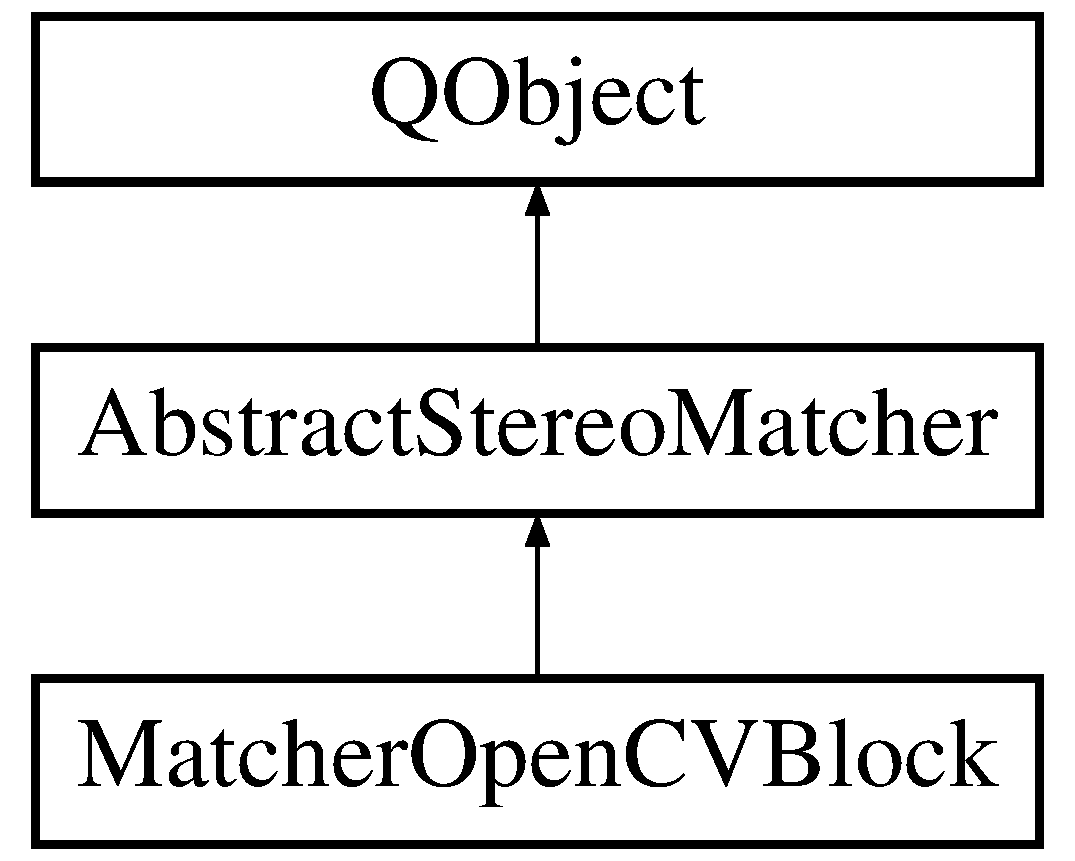
\includegraphics[height=3.000000cm]{class_matcher_open_c_v_block}
\end{center}
\end{figure}
\subsection*{Public Slots}
\begin{DoxyCompactItemize}
\item 
\hypertarget{class_matcher_open_c_v_block_a0eb06c5ced42857eda54abc71cc86746}{}void {\bfseries set\+Min\+Disparity} (int min\+\_\+disparity)\label{class_matcher_open_c_v_block_a0eb06c5ced42857eda54abc71cc86746}

\item 
\hypertarget{class_matcher_open_c_v_block_a8c4b003fdcdd3be586dee4c5ae0cd81f}{}void {\bfseries set\+Disparity\+Range} (int disparity\+\_\+range)\label{class_matcher_open_c_v_block_a8c4b003fdcdd3be586dee4c5ae0cd81f}

\item 
\hypertarget{class_matcher_open_c_v_block_a4a34614f23f03c4505f6dcde975ca3cc}{}void {\bfseries set\+Block\+Size} (int block\+\_\+size)\label{class_matcher_open_c_v_block_a4a34614f23f03c4505f6dcde975ca3cc}

\item 
\hypertarget{class_matcher_open_c_v_block_a929bdcd0ddc2d0e64a83d9b467226a45}{}void {\bfseries set\+Disp12\+Max\+Diff} (int diff)\label{class_matcher_open_c_v_block_a929bdcd0ddc2d0e64a83d9b467226a45}

\item 
\hypertarget{class_matcher_open_c_v_block_a210b7cf4f75d7507643af3a826695aa6}{}void {\bfseries set\+Prefilter\+Type} (int type)\label{class_matcher_open_c_v_block_a210b7cf4f75d7507643af3a826695aa6}

\item 
\hypertarget{class_matcher_open_c_v_block_acee691720a3fe7c796dbbf74f7a06da4}{}void {\bfseries set\+Prefilter\+Size} (int size)\label{class_matcher_open_c_v_block_acee691720a3fe7c796dbbf74f7a06da4}

\item 
\hypertarget{class_matcher_open_c_v_block_a4ee85d786a4feb635151cfd4bb656564}{}void {\bfseries set\+Prefilter\+Cap} (int cap)\label{class_matcher_open_c_v_block_a4ee85d786a4feb635151cfd4bb656564}

\item 
\hypertarget{class_matcher_open_c_v_block_a668eaeb56744a3982d90a1e7b1c5ead7}{}void {\bfseries set\+Texture\+Threshold} (int threshold)\label{class_matcher_open_c_v_block_a668eaeb56744a3982d90a1e7b1c5ead7}

\item 
\hypertarget{class_matcher_open_c_v_block_ae6d8ad706c2743abc1998a7e7deae899}{}void {\bfseries set\+Uniqueness\+Ratio} (int ratio)\label{class_matcher_open_c_v_block_ae6d8ad706c2743abc1998a7e7deae899}

\item 
\hypertarget{class_matcher_open_c_v_block_a0ff44917c41ed78c3fa70fa569b704b4}{}void {\bfseries set\+Speckle\+Filter\+Window} (int window)\label{class_matcher_open_c_v_block_a0ff44917c41ed78c3fa70fa569b704b4}

\item 
\hypertarget{class_matcher_open_c_v_block_a5273db5b920ac74d5d141efaeaa8a3bb}{}void {\bfseries set\+Speckle\+Filter\+Range} (int range)\label{class_matcher_open_c_v_block_a5273db5b920ac74d5d141efaeaa8a3bb}

\item 
\hypertarget{class_matcher_open_c_v_block_a4ee38d692807aaaece7139f591ca76e3}{}int {\bfseries get\+Error\+Disparity} (void)\label{class_matcher_open_c_v_block_a4ee38d692807aaaece7139f591ca76e3}

\item 
\hypertarget{class_matcher_open_c_v_block_a70f79ecf99481ebd858a1cf055b8cc59}{}int {\bfseries get\+Min\+Disparity} ()\label{class_matcher_open_c_v_block_a70f79ecf99481ebd858a1cf055b8cc59}

\item 
\hypertarget{class_matcher_open_c_v_block_aa6cb3a70729a5602f688608324a19655}{}int {\bfseries get\+Disparity\+Range} ()\label{class_matcher_open_c_v_block_aa6cb3a70729a5602f688608324a19655}

\item 
\hypertarget{class_matcher_open_c_v_block_a48761cf09adce564a9fdaa91d25c037e}{}int {\bfseries get\+Block\+Size} ()\label{class_matcher_open_c_v_block_a48761cf09adce564a9fdaa91d25c037e}

\item 
\hypertarget{class_matcher_open_c_v_block_afbff703a45d2a1a80c73682a60c6239b}{}int {\bfseries get\+Disp12\+Max\+Diff} ()\label{class_matcher_open_c_v_block_afbff703a45d2a1a80c73682a60c6239b}

\item 
\hypertarget{class_matcher_open_c_v_block_a88ab7c98478d047698ad940fe165d4ed}{}int {\bfseries get\+Prefilter\+Type} ()\label{class_matcher_open_c_v_block_a88ab7c98478d047698ad940fe165d4ed}

\item 
\hypertarget{class_matcher_open_c_v_block_a976b0f99c4b0aa56a51cab814b93f82a}{}int {\bfseries get\+Prefilter\+Size} ()\label{class_matcher_open_c_v_block_a976b0f99c4b0aa56a51cab814b93f82a}

\item 
\hypertarget{class_matcher_open_c_v_block_a22acb450db7fada0a87750951c26f4b5}{}int {\bfseries get\+Prefilter\+Cap} ()\label{class_matcher_open_c_v_block_a22acb450db7fada0a87750951c26f4b5}

\item 
\hypertarget{class_matcher_open_c_v_block_aab48ecee03a3c961d47ebc087b45a820}{}int {\bfseries get\+Texture\+Threshold} ()\label{class_matcher_open_c_v_block_aab48ecee03a3c961d47ebc087b45a820}

\item 
\hypertarget{class_matcher_open_c_v_block_a9c9ed77a220f19e79b35ac6b0e6d1fc4}{}int {\bfseries get\+Uniqueness\+Ratio} ()\label{class_matcher_open_c_v_block_a9c9ed77a220f19e79b35ac6b0e6d1fc4}

\item 
\hypertarget{class_matcher_open_c_v_block_a9190ab77f353a5fb3bde1ead371802b0}{}int {\bfseries get\+Speckle\+Filter\+Window} ()\label{class_matcher_open_c_v_block_a9190ab77f353a5fb3bde1ead371802b0}

\item 
\hypertarget{class_matcher_open_c_v_block_a69f73917c0acafd723fdafb6a915c14c}{}int {\bfseries get\+Speckle\+Filter\+Range} ()\label{class_matcher_open_c_v_block_a69f73917c0acafd723fdafb6a915c14c}

\item 
\hypertarget{class_matcher_open_c_v_block_ae5ec6be50177c4540668ee1508c84de0}{}void {\bfseries save\+Params} ()\label{class_matcher_open_c_v_block_ae5ec6be50177c4540668ee1508c84de0}

\item 
\hypertarget{class_matcher_open_c_v_block_a2abcf69b70bed18c59609b1a432a3fbd}{}void {\bfseries forward\+Match} (void)\label{class_matcher_open_c_v_block_a2abcf69b70bed18c59609b1a432a3fbd}

\item 
\hypertarget{class_matcher_open_c_v_block_a7c31fc9dbe970b3cf7e01a0f1c5baf60}{}void {\bfseries backward\+Match} (void)\label{class_matcher_open_c_v_block_a7c31fc9dbe970b3cf7e01a0f1c5baf60}

\end{DoxyCompactItemize}
\subsection*{Public Member Functions}
\begin{DoxyCompactItemize}
\item 
\hypertarget{class_matcher_open_c_v_block_a8299a5da1c1a66530dab107e7cda885f}{}{\bfseries Matcher\+Open\+C\+V\+Block} (Q\+Object $\ast$parent=0, cv\+::\+Size image\+\_\+size=cv\+::\+Size(0, 0))\label{class_matcher_open_c_v_block_a8299a5da1c1a66530dab107e7cda885f}

\end{DoxyCompactItemize}
\subsection*{Additional Inherited Members}


\subsection{Detailed Description}


Definition at line 12 of file matcheropencvblock.\+h.



The documentation for this class was generated from the following files\+:\begin{DoxyCompactItemize}
\item 
src/matcheropencvblock.\+h\item 
src/matcheropencvblock.\+cpp\end{DoxyCompactItemize}

\hypertarget{class_matcher_open_c_v_s_g_b_m}{}\section{Matcher\+Open\+C\+V\+S\+G\+B\+M Class Reference}
\label{class_matcher_open_c_v_s_g_b_m}\index{Matcher\+Open\+C\+V\+S\+G\+B\+M@{Matcher\+Open\+C\+V\+S\+G\+B\+M}}
Inheritance diagram for Matcher\+Open\+C\+V\+S\+G\+B\+M\+:\begin{figure}[H]
\begin{center}
\leavevmode
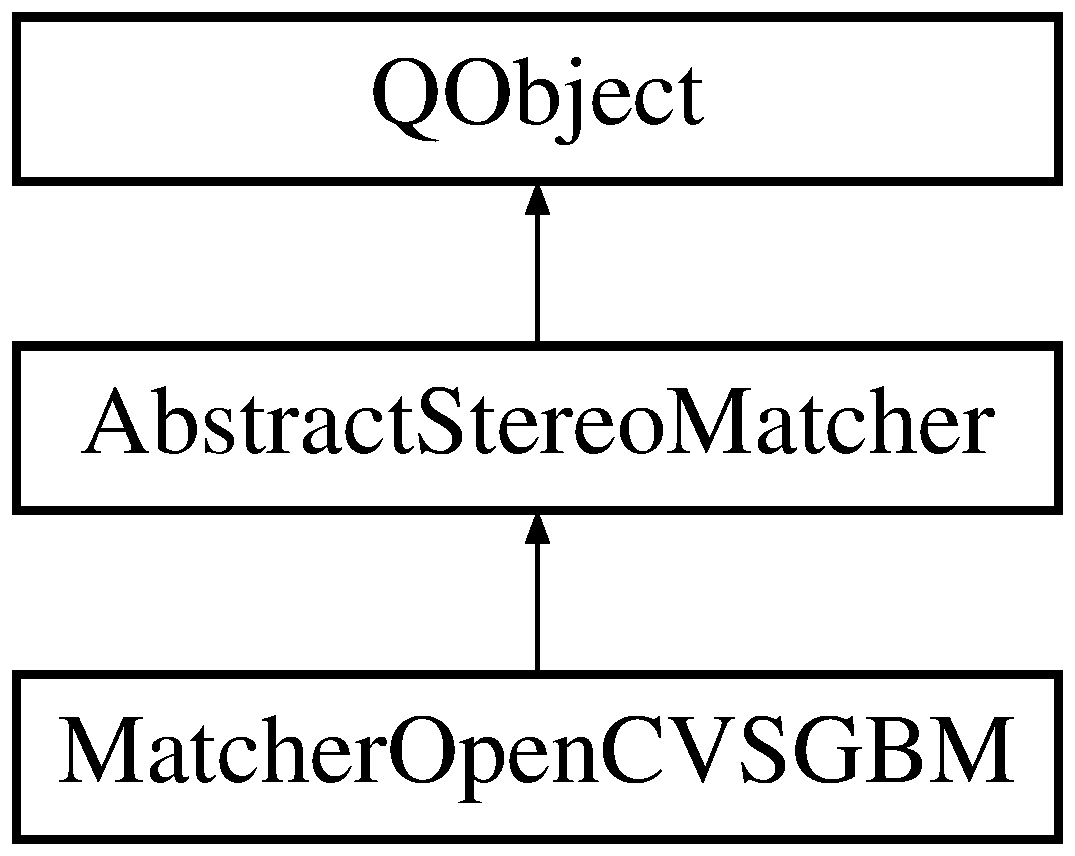
\includegraphics[height=3.000000cm]{class_matcher_open_c_v_s_g_b_m}
\end{center}
\end{figure}
\subsection*{Public Slots}
\begin{DoxyCompactItemize}
\item 
\hypertarget{class_matcher_open_c_v_s_g_b_m_aeda34d7537939c8feb1bd085b37333e9}{}void {\bfseries set\+Min\+Disparity} (int min\+\_\+disparity)\label{class_matcher_open_c_v_s_g_b_m_aeda34d7537939c8feb1bd085b37333e9}

\item 
\hypertarget{class_matcher_open_c_v_s_g_b_m_a7b8de74c1ba55bd10127145fe0f135e9}{}void {\bfseries set\+Disparity\+Range} (int disparity\+\_\+range)\label{class_matcher_open_c_v_s_g_b_m_a7b8de74c1ba55bd10127145fe0f135e9}

\item 
\hypertarget{class_matcher_open_c_v_s_g_b_m_afb8e186fd35dc7830afbea0f525025e7}{}void {\bfseries set\+Block\+Size} (int block\+\_\+size)\label{class_matcher_open_c_v_s_g_b_m_afb8e186fd35dc7830afbea0f525025e7}

\item 
\hypertarget{class_matcher_open_c_v_s_g_b_m_a27a251f5645a7ebc813290aec5b2fea6}{}void {\bfseries set\+Disp12\+Max\+Diff} (int diff)\label{class_matcher_open_c_v_s_g_b_m_a27a251f5645a7ebc813290aec5b2fea6}

\item 
\hypertarget{class_matcher_open_c_v_s_g_b_m_a9e7548ef4d0e13312aa2e0836e8714af}{}void {\bfseries set\+Uniqueness\+Ratio} (int ratio)\label{class_matcher_open_c_v_s_g_b_m_a9e7548ef4d0e13312aa2e0836e8714af}

\item 
\hypertarget{class_matcher_open_c_v_s_g_b_m_a66e9c8a8087464e291a90c5b0dd9e795}{}void {\bfseries set\+Speckle\+Filter\+Window} (int window)\label{class_matcher_open_c_v_s_g_b_m_a66e9c8a8087464e291a90c5b0dd9e795}

\item 
\hypertarget{class_matcher_open_c_v_s_g_b_m_a8d6cb3200204af80a2f7ef228b51526e}{}void {\bfseries set\+Speckle\+Filter\+Range} (int range)\label{class_matcher_open_c_v_s_g_b_m_a8d6cb3200204af80a2f7ef228b51526e}

\item 
\hypertarget{class_matcher_open_c_v_s_g_b_m_a96524a760c1bb475e8bf306db7d39c66}{}int {\bfseries get\+Error\+Disparity} (void)\label{class_matcher_open_c_v_s_g_b_m_a96524a760c1bb475e8bf306db7d39c66}

\item 
\hypertarget{class_matcher_open_c_v_s_g_b_m_a45225a59cee1727abce90e6dea990418}{}void {\bfseries save\+Params} ()\label{class_matcher_open_c_v_s_g_b_m_a45225a59cee1727abce90e6dea990418}

\item 
\hypertarget{class_matcher_open_c_v_s_g_b_m_a10443707c8205bb90461fd6b4f8e79d8}{}void {\bfseries forward\+Match} (void)\label{class_matcher_open_c_v_s_g_b_m_a10443707c8205bb90461fd6b4f8e79d8}

\item 
\hypertarget{class_matcher_open_c_v_s_g_b_m_a3cd2e33926c85e87df779badc5a86f51}{}void {\bfseries backward\+Match} (void)\label{class_matcher_open_c_v_s_g_b_m_a3cd2e33926c85e87df779badc5a86f51}

\item 
\hypertarget{class_matcher_open_c_v_s_g_b_m_a525af9c2a3e1ae04c5e3de33e80cf3ca}{}int {\bfseries get\+Min\+Disparity} ()\label{class_matcher_open_c_v_s_g_b_m_a525af9c2a3e1ae04c5e3de33e80cf3ca}

\item 
\hypertarget{class_matcher_open_c_v_s_g_b_m_a30e6692b076c5adf8ef1e1584c03202a}{}int {\bfseries get\+Disparity\+Range} ()\label{class_matcher_open_c_v_s_g_b_m_a30e6692b076c5adf8ef1e1584c03202a}

\item 
\hypertarget{class_matcher_open_c_v_s_g_b_m_a995f6a2e469eb9b3412b37c1da5ea16c}{}int {\bfseries get\+Block\+Size} ()\label{class_matcher_open_c_v_s_g_b_m_a995f6a2e469eb9b3412b37c1da5ea16c}

\item 
\hypertarget{class_matcher_open_c_v_s_g_b_m_a8fe62c6d80597541d02c18709d9516d2}{}int {\bfseries get\+Disp12\+Max\+Diff} ()\label{class_matcher_open_c_v_s_g_b_m_a8fe62c6d80597541d02c18709d9516d2}

\item 
\hypertarget{class_matcher_open_c_v_s_g_b_m_ad47daedbb87aeb15dba6992978f1969d}{}int {\bfseries get\+Prefilter\+Cap} ()\label{class_matcher_open_c_v_s_g_b_m_ad47daedbb87aeb15dba6992978f1969d}

\item 
\hypertarget{class_matcher_open_c_v_s_g_b_m_aef6c00036288432502b1280d642a4263}{}int {\bfseries get\+Uniqueness\+Ratio} ()\label{class_matcher_open_c_v_s_g_b_m_aef6c00036288432502b1280d642a4263}

\item 
\hypertarget{class_matcher_open_c_v_s_g_b_m_a66f6f114d0e2a0a9a17ef7469a9a328e}{}int {\bfseries get\+Speckle\+Filter\+Window} ()\label{class_matcher_open_c_v_s_g_b_m_a66f6f114d0e2a0a9a17ef7469a9a328e}

\item 
\hypertarget{class_matcher_open_c_v_s_g_b_m_a1de219c9420b8549fc3b5a67d491128b}{}int {\bfseries get\+Speckle\+Filter\+Range} ()\label{class_matcher_open_c_v_s_g_b_m_a1de219c9420b8549fc3b5a67d491128b}

\end{DoxyCompactItemize}
\subsection*{Public Member Functions}
\begin{DoxyCompactItemize}
\item 
\hypertarget{class_matcher_open_c_v_s_g_b_m_ac6e50ab709cd3a87bde9b47dca8f92f0}{}{\bfseries Matcher\+Open\+C\+V\+S\+G\+B\+M} (Q\+Object $\ast$parent=0, cv\+::\+Size image\+\_\+size=cv\+::\+Size(0, 0))\label{class_matcher_open_c_v_s_g_b_m_ac6e50ab709cd3a87bde9b47dca8f92f0}

\end{DoxyCompactItemize}
\subsection*{Additional Inherited Members}


\subsection{Detailed Description}


Definition at line 12 of file matcheropencvsgbm.\+h.



The documentation for this class was generated from the following files\+:\begin{DoxyCompactItemize}
\item 
src/matcheropencvsgbm.\+h\item 
src/matcheropencvsgbm.\+cpp\end{DoxyCompactItemize}

\hypertarget{class_matcher_widget}{}\section{Matcher\+Widget Class Reference}
\label{class_matcher_widget}\index{Matcher\+Widget@{Matcher\+Widget}}
Inheritance diagram for Matcher\+Widget\+:\begin{figure}[H]
\begin{center}
\leavevmode
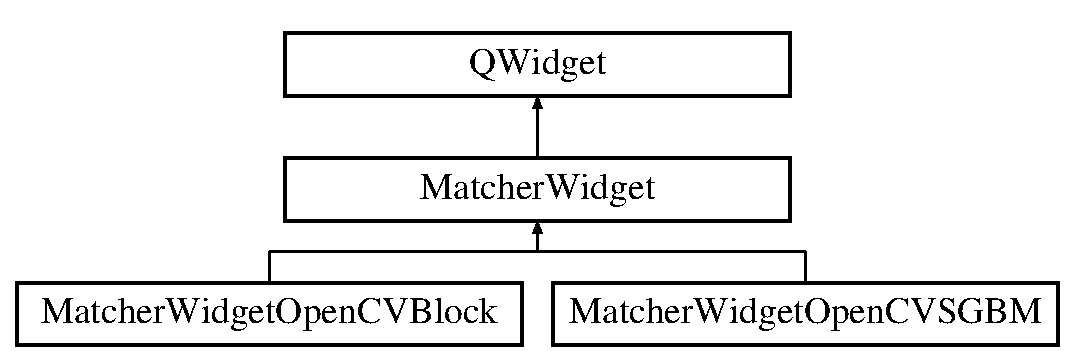
\includegraphics[height=3.000000cm]{class_matcher_widget}
\end{center}
\end{figure}
\subsection*{Public Member Functions}
\begin{DoxyCompactItemize}
\item 
\hypertarget{class_matcher_widget_a2200fa2bb5a1bffcc4552f63ca1bdb5d}{}{\bfseries Matcher\+Widget} (Q\+Widget $\ast$parent=0)\label{class_matcher_widget_a2200fa2bb5a1bffcc4552f63ca1bdb5d}

\item 
\hypertarget{class_matcher_widget_ab288c58c635180941360691cfde3e677}{}virtual \hyperlink{class_abstract_stereo_matcher}{Abstract\+Stereo\+Matcher} $\ast$ {\bfseries get\+Matcher} (void)=0\label{class_matcher_widget_ab288c58c635180941360691cfde3e677}

\end{DoxyCompactItemize}


\subsection{Detailed Description}


Definition at line 12 of file matcherwidget.\+h.



The documentation for this class was generated from the following file\+:\begin{DoxyCompactItemize}
\item 
src/matcherwidget.\+h\end{DoxyCompactItemize}

\hypertarget{class_matcher_widget_open_c_v_block}{}\section{Matcher\+Widget\+Open\+C\+V\+Block Class Reference}
\label{class_matcher_widget_open_c_v_block}\index{Matcher\+Widget\+Open\+C\+V\+Block@{Matcher\+Widget\+Open\+C\+V\+Block}}
Inheritance diagram for Matcher\+Widget\+Open\+C\+V\+Block\+:\begin{figure}[H]
\begin{center}
\leavevmode
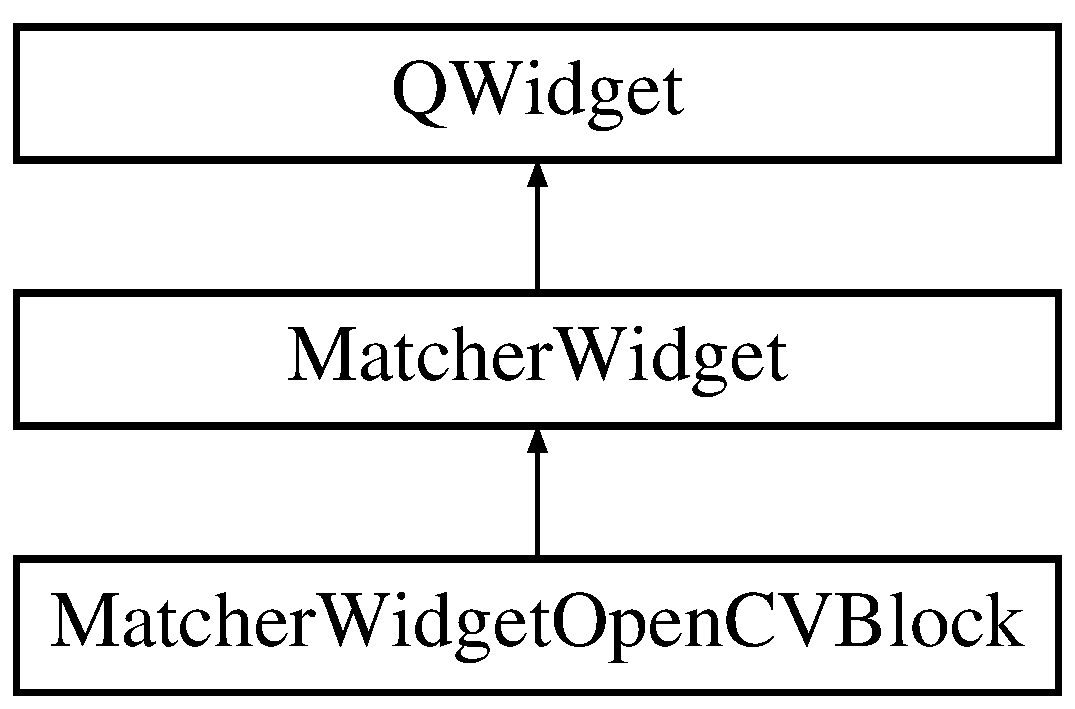
\includegraphics[height=3.000000cm]{class_matcher_widget_open_c_v_block}
\end{center}
\end{figure}
\subsection*{Public Slots}
\begin{DoxyCompactItemize}
\item 
\hypertarget{class_matcher_widget_open_c_v_block_a50c22ff2dd4734f2cb21dfbfaf645b88}{}void {\bfseries update\+Disparity\+Range} (int)\label{class_matcher_widget_open_c_v_block_a50c22ff2dd4734f2cb21dfbfaf645b88}

\item 
\hypertarget{class_matcher_widget_open_c_v_block_a4a31dd4d9bb6a292d5c1c090da27051e}{}void {\bfseries update\+Block\+Size} (int)\label{class_matcher_widget_open_c_v_block_a4a31dd4d9bb6a292d5c1c090da27051e}

\item 
\hypertarget{class_matcher_widget_open_c_v_block_aab13b7581e24763091f1d522d64dddd8}{}void {\bfseries update\+Min\+Disparity} (int)\label{class_matcher_widget_open_c_v_block_aab13b7581e24763091f1d522d64dddd8}

\item 
\hypertarget{class_matcher_widget_open_c_v_block_ad7bd35d1517af81af30372cc34c7c069}{}void {\bfseries update\+Prefilter\+Cap} (int cap)\label{class_matcher_widget_open_c_v_block_ad7bd35d1517af81af30372cc34c7c069}

\item 
\hypertarget{class_matcher_widget_open_c_v_block_acee1c5e53f54825913d4fca47630c787}{}void {\bfseries update\+Prefilter\+Size} (int size)\label{class_matcher_widget_open_c_v_block_acee1c5e53f54825913d4fca47630c787}

\item 
\hypertarget{class_matcher_widget_open_c_v_block_ac75ba57e87773af65b936f7128b0089a}{}void {\bfseries update\+Prefilter\+Type} (int index)\label{class_matcher_widget_open_c_v_block_ac75ba57e87773af65b936f7128b0089a}

\item 
\hypertarget{class_matcher_widget_open_c_v_block_a2f60d99056426b7e40ae89eea270dd50}{}void {\bfseries update\+Texture\+Threshold} (int threshold)\label{class_matcher_widget_open_c_v_block_a2f60d99056426b7e40ae89eea270dd50}

\item 
\hypertarget{class_matcher_widget_open_c_v_block_a4cce5ad7783756b764c208839fd4d7a4}{}void {\bfseries update\+Consistency} (int consistency)\label{class_matcher_widget_open_c_v_block_a4cce5ad7783756b764c208839fd4d7a4}

\item 
\hypertarget{class_matcher_widget_open_c_v_block_a45f8d8c92b9441de897dfc30a2e8fa95}{}void {\bfseries update\+Uniqueness\+Ratio} (int ratio)\label{class_matcher_widget_open_c_v_block_a45f8d8c92b9441de897dfc30a2e8fa95}

\item 
\hypertarget{class_matcher_widget_open_c_v_block_ad82ae3302a5c11b09d5b0f1bdf4d3366}{}void {\bfseries update\+Speckle\+Range} (int range)\label{class_matcher_widget_open_c_v_block_ad82ae3302a5c11b09d5b0f1bdf4d3366}

\item 
\hypertarget{class_matcher_widget_open_c_v_block_ab5f328a18e994ff6195734486f366202}{}void {\bfseries update\+Speckle\+Window} (int window)\label{class_matcher_widget_open_c_v_block_ab5f328a18e994ff6195734486f366202}

\item 
\hypertarget{class_matcher_widget_open_c_v_block_a5139f63b5c756006b10bb29b6748a7a7}{}void {\bfseries enable\+Speckle\+Filter} (bool enable)\label{class_matcher_widget_open_c_v_block_a5139f63b5c756006b10bb29b6748a7a7}

\item 
\hypertarget{class_matcher_widget_open_c_v_block_a92dce6487b98632411a55353cec5d76e}{}void {\bfseries enable\+Consistency} (bool enable)\label{class_matcher_widget_open_c_v_block_a92dce6487b98632411a55353cec5d76e}

\item 
\hypertarget{class_matcher_widget_open_c_v_block_af7c6bef8f8db89d6accdbf3ce551b7a4}{}\hyperlink{class_abstract_stereo_matcher}{Abstract\+Stereo\+Matcher} $\ast$ {\bfseries get\+Matcher} (void)\label{class_matcher_widget_open_c_v_block_af7c6bef8f8db89d6accdbf3ce551b7a4}

\item 
\hypertarget{class_matcher_widget_open_c_v_block_a106a9d2af50ffe2d07399a89fc9df1c1}{}void {\bfseries on\+Save\+Clicked} ()\label{class_matcher_widget_open_c_v_block_a106a9d2af50ffe2d07399a89fc9df1c1}

\end{DoxyCompactItemize}
\subsection*{Signals}
\begin{DoxyCompactItemize}
\item 
\hypertarget{class_matcher_widget_open_c_v_block_afff4da21bf63fbc4999002a068908f3d}{}void {\bfseries min\+Disparity} (int)\label{class_matcher_widget_open_c_v_block_afff4da21bf63fbc4999002a068908f3d}

\item 
\hypertarget{class_matcher_widget_open_c_v_block_a1a04a88e8b886ebc922480a318b9f79e}{}void {\bfseries disparity\+Range} (int)\label{class_matcher_widget_open_c_v_block_a1a04a88e8b886ebc922480a318b9f79e}

\item 
\hypertarget{class_matcher_widget_open_c_v_block_a61948671169d0754115a4acc5f6ab542}{}void {\bfseries block\+Size} (int)\label{class_matcher_widget_open_c_v_block_a61948671169d0754115a4acc5f6ab542}

\item 
\hypertarget{class_matcher_widget_open_c_v_block_a7182b843fc31452f43226ffa27355ef0}{}void {\bfseries prefilter\+Cap} (int)\label{class_matcher_widget_open_c_v_block_a7182b843fc31452f43226ffa27355ef0}

\item 
\hypertarget{class_matcher_widget_open_c_v_block_a25f55b2aa65376bb0356fb9c578a822c}{}void {\bfseries prefilter\+Size} (int)\label{class_matcher_widget_open_c_v_block_a25f55b2aa65376bb0356fb9c578a822c}

\item 
\hypertarget{class_matcher_widget_open_c_v_block_a1dc8ded18f7bc17d81127ecc443f6b47}{}void {\bfseries prefilter\+Type} (int)\label{class_matcher_widget_open_c_v_block_a1dc8ded18f7bc17d81127ecc443f6b47}

\item 
\hypertarget{class_matcher_widget_open_c_v_block_a39dde3fecc67cc09a8ea80bfde1f6ab9}{}void {\bfseries texture\+Threshold} (int)\label{class_matcher_widget_open_c_v_block_a39dde3fecc67cc09a8ea80bfde1f6ab9}

\item 
\hypertarget{class_matcher_widget_open_c_v_block_a72aced627227becd1873ee1895da1e60}{}void {\bfseries speckle\+Window} (int)\label{class_matcher_widget_open_c_v_block_a72aced627227becd1873ee1895da1e60}

\item 
\hypertarget{class_matcher_widget_open_c_v_block_a01f425b6f399633b38ce3e6e91492e00}{}void {\bfseries speckle\+Range} (int)\label{class_matcher_widget_open_c_v_block_a01f425b6f399633b38ce3e6e91492e00}

\item 
\hypertarget{class_matcher_widget_open_c_v_block_ad07b256a3f33dd3b0b3554e73ed6abdc}{}void {\bfseries consistency} (int)\label{class_matcher_widget_open_c_v_block_ad07b256a3f33dd3b0b3554e73ed6abdc}

\item 
\hypertarget{class_matcher_widget_open_c_v_block_a1ba1a1ff91c6a455528af613b972f882}{}void {\bfseries uniqueness\+Ratio} (int)\label{class_matcher_widget_open_c_v_block_a1ba1a1ff91c6a455528af613b972f882}

\item 
\hypertarget{class_matcher_widget_open_c_v_block_a9c2f7a6be57cbf63079f2b32411c433c}{}void {\bfseries save\+Clicked} ()\label{class_matcher_widget_open_c_v_block_a9c2f7a6be57cbf63079f2b32411c433c}

\end{DoxyCompactItemize}
\subsection*{Public Member Functions}
\begin{DoxyCompactItemize}
\item 
\hypertarget{class_matcher_widget_open_c_v_block_a5f2d21ee8c7a9c429e251a4c1b470dae}{}{\bfseries Matcher\+Widget\+Open\+C\+V\+Block} (Q\+Widget $\ast$parent=0, cv\+::\+Size image\+\_\+size=cv\+::\+Size(0, 0))\label{class_matcher_widget_open_c_v_block_a5f2d21ee8c7a9c429e251a4c1b470dae}

\item 
\hypertarget{class_matcher_widget_open_c_v_block_a61613853ca6da5ed7ab349ef64833be5}{}void {\bfseries set\+Image\+Width} (int width)\label{class_matcher_widget_open_c_v_block_a61613853ca6da5ed7ab349ef64833be5}

\end{DoxyCompactItemize}


\subsection{Detailed Description}


Definition at line 17 of file matcherwidgetopencvblock.\+h.



The documentation for this class was generated from the following files\+:\begin{DoxyCompactItemize}
\item 
src/matcherwidgetopencvblock.\+h\item 
src/matcherwidgetopencvblock.\+cpp\end{DoxyCompactItemize}

\hypertarget{class_matcher_widget_open_c_v_s_g_b_m}{}\section{Matcher\+Widget\+Open\+C\+V\+S\+G\+B\+M Class Reference}
\label{class_matcher_widget_open_c_v_s_g_b_m}\index{Matcher\+Widget\+Open\+C\+V\+S\+G\+B\+M@{Matcher\+Widget\+Open\+C\+V\+S\+G\+B\+M}}
Inheritance diagram for Matcher\+Widget\+Open\+C\+V\+S\+G\+B\+M\+:\begin{figure}[H]
\begin{center}
\leavevmode
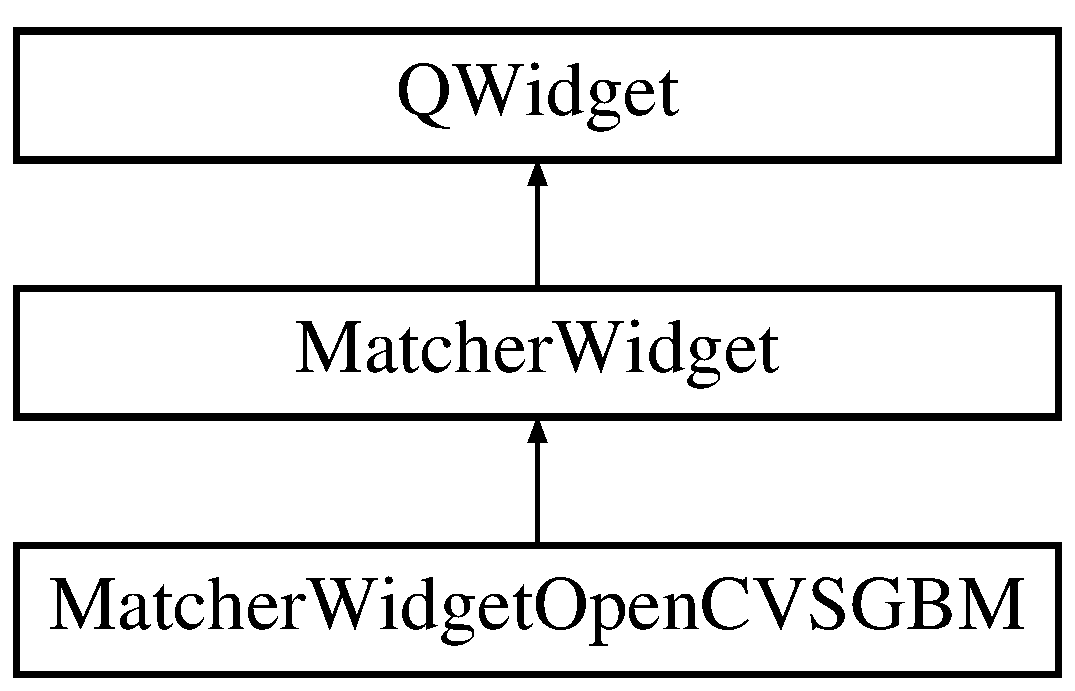
\includegraphics[height=3.000000cm]{class_matcher_widget_open_c_v_s_g_b_m}
\end{center}
\end{figure}
\subsection*{Public Slots}
\begin{DoxyCompactItemize}
\item 
\hypertarget{class_matcher_widget_open_c_v_s_g_b_m_a58ea3c13fd89422e87ce8c13416e2f5b}{}void {\bfseries update\+Disparity\+Range} (int)\label{class_matcher_widget_open_c_v_s_g_b_m_a58ea3c13fd89422e87ce8c13416e2f5b}

\item 
\hypertarget{class_matcher_widget_open_c_v_s_g_b_m_aa67aa1f2e820eaf7d5a4937fea2bd454}{}void {\bfseries update\+Block\+Size} (int)\label{class_matcher_widget_open_c_v_s_g_b_m_aa67aa1f2e820eaf7d5a4937fea2bd454}

\item 
\hypertarget{class_matcher_widget_open_c_v_s_g_b_m_a2b1642362087e02dbef29d4251827541}{}void {\bfseries update\+Min\+Disparity} (int)\label{class_matcher_widget_open_c_v_s_g_b_m_a2b1642362087e02dbef29d4251827541}

\item 
\hypertarget{class_matcher_widget_open_c_v_s_g_b_m_a323c64dced050d93c85a982052b30b18}{}void {\bfseries update\+Consistency} (int consistency)\label{class_matcher_widget_open_c_v_s_g_b_m_a323c64dced050d93c85a982052b30b18}

\item 
\hypertarget{class_matcher_widget_open_c_v_s_g_b_m_a572ca91cc9740e30ab1ea221b952db0b}{}void {\bfseries update\+Uniqueness\+Ratio} (int ratio)\label{class_matcher_widget_open_c_v_s_g_b_m_a572ca91cc9740e30ab1ea221b952db0b}

\item 
\hypertarget{class_matcher_widget_open_c_v_s_g_b_m_a11eeef877a92b5b9829091f95ef46fcc}{}void {\bfseries update\+Speckle\+Range} (int range)\label{class_matcher_widget_open_c_v_s_g_b_m_a11eeef877a92b5b9829091f95ef46fcc}

\item 
\hypertarget{class_matcher_widget_open_c_v_s_g_b_m_a9db7a9916b30317a409c536b0b0745f6}{}void {\bfseries update\+Speckle\+Window} (int window)\label{class_matcher_widget_open_c_v_s_g_b_m_a9db7a9916b30317a409c536b0b0745f6}

\item 
\hypertarget{class_matcher_widget_open_c_v_s_g_b_m_a3b0438995da832995ee30fc44c0ca45f}{}void {\bfseries enable\+Speckle\+Filter} (bool enable)\label{class_matcher_widget_open_c_v_s_g_b_m_a3b0438995da832995ee30fc44c0ca45f}

\item 
\hypertarget{class_matcher_widget_open_c_v_s_g_b_m_a23941782ed2ef9cc9e8748929e2c6d40}{}void {\bfseries enable\+Consistency} (bool enable)\label{class_matcher_widget_open_c_v_s_g_b_m_a23941782ed2ef9cc9e8748929e2c6d40}

\item 
\hypertarget{class_matcher_widget_open_c_v_s_g_b_m_a2e792ea7fb0f07b482ba7dabeade4a4f}{}\hyperlink{class_abstract_stereo_matcher}{Abstract\+Stereo\+Matcher} $\ast$ {\bfseries get\+Matcher} (void)\label{class_matcher_widget_open_c_v_s_g_b_m_a2e792ea7fb0f07b482ba7dabeade4a4f}

\item 
\hypertarget{class_matcher_widget_open_c_v_s_g_b_m_a4baa468def1b004f9e783694901bb5de}{}void {\bfseries on\+Save\+Clicked} ()\label{class_matcher_widget_open_c_v_s_g_b_m_a4baa468def1b004f9e783694901bb5de}

\end{DoxyCompactItemize}
\subsection*{Signals}
\begin{DoxyCompactItemize}
\item 
\hypertarget{class_matcher_widget_open_c_v_s_g_b_m_a894a5cbe9aa8f8e076a02c4a25f4ddc5}{}void {\bfseries min\+Disparity} (int)\label{class_matcher_widget_open_c_v_s_g_b_m_a894a5cbe9aa8f8e076a02c4a25f4ddc5}

\item 
\hypertarget{class_matcher_widget_open_c_v_s_g_b_m_a8260b459dab3e11593bd479d51424604}{}void {\bfseries disparity\+Range} (int)\label{class_matcher_widget_open_c_v_s_g_b_m_a8260b459dab3e11593bd479d51424604}

\item 
\hypertarget{class_matcher_widget_open_c_v_s_g_b_m_ab0e364c6037230323e797c3aa64dd7fd}{}void {\bfseries block\+Size} (int)\label{class_matcher_widget_open_c_v_s_g_b_m_ab0e364c6037230323e797c3aa64dd7fd}

\item 
\hypertarget{class_matcher_widget_open_c_v_s_g_b_m_af3cafa4ad8cc31c5ec1bb04564d41cab}{}void {\bfseries speckle\+Window} (int)\label{class_matcher_widget_open_c_v_s_g_b_m_af3cafa4ad8cc31c5ec1bb04564d41cab}

\item 
\hypertarget{class_matcher_widget_open_c_v_s_g_b_m_ac306ee75119e8812eb52e57daba44ba5}{}void {\bfseries speckle\+Range} (int)\label{class_matcher_widget_open_c_v_s_g_b_m_ac306ee75119e8812eb52e57daba44ba5}

\item 
\hypertarget{class_matcher_widget_open_c_v_s_g_b_m_a94adb6bd93794a0a1b68ce867c80af6b}{}void {\bfseries consistency} (int)\label{class_matcher_widget_open_c_v_s_g_b_m_a94adb6bd93794a0a1b68ce867c80af6b}

\item 
\hypertarget{class_matcher_widget_open_c_v_s_g_b_m_a4585ab4a4514df788faabd649740938e}{}void {\bfseries uniqueness\+Ratio} (int)\label{class_matcher_widget_open_c_v_s_g_b_m_a4585ab4a4514df788faabd649740938e}

\item 
\hypertarget{class_matcher_widget_open_c_v_s_g_b_m_af4a10daeacbd7367e2aacad5836bb0e2}{}void {\bfseries save\+Clicked} ()\label{class_matcher_widget_open_c_v_s_g_b_m_af4a10daeacbd7367e2aacad5836bb0e2}

\end{DoxyCompactItemize}
\subsection*{Public Member Functions}
\begin{DoxyCompactItemize}
\item 
\hypertarget{class_matcher_widget_open_c_v_s_g_b_m_a86cb7fbd720567c33abf2548c7cf8589}{}{\bfseries Matcher\+Widget\+Open\+C\+V\+S\+G\+B\+M} (Q\+Widget $\ast$parent=0, cv\+::\+Size image\+\_\+size=cv\+::\+Size(0, 0))\label{class_matcher_widget_open_c_v_s_g_b_m_a86cb7fbd720567c33abf2548c7cf8589}

\item 
\hypertarget{class_matcher_widget_open_c_v_s_g_b_m_ab3a74b9e526e919475065fd8953c49c2}{}void {\bfseries set\+Image\+Width} (int width)\label{class_matcher_widget_open_c_v_s_g_b_m_ab3a74b9e526e919475065fd8953c49c2}

\end{DoxyCompactItemize}


\subsection{Detailed Description}


Definition at line 17 of file matcherwidgetopencvsgbm.\+h.



The documentation for this class was generated from the following files\+:\begin{DoxyCompactItemize}
\item 
src/matcherwidgetopencvsgbm.\+h\item 
src/matcherwidgetopencvsgbm.\+cpp\end{DoxyCompactItemize}

\hypertarget{class_param_file}{}\section{Param\+File Class Reference}
\label{class_param_file}\index{Param\+File@{Param\+File}}
\subsection*{Public Member Functions}
\begin{DoxyCompactItemize}
\item 
\hypertarget{class_param_file_a161af51d06ed58444b0de69f05215692}{}void {\bfseries update\+Previous\+Directory} (Q\+String dir)\label{class_param_file_a161af51d06ed58444b0de69f05215692}

\item 
\hypertarget{class_param_file_a3ea5e819ddbaffce3e817ea9a605f08a}{}Q\+String {\bfseries get} (Q\+String tag\+Name)\label{class_param_file_a3ea5e819ddbaffce3e817ea9a605f08a}

\item 
\hypertarget{class_param_file_a02ec327dc82b36bb00aa2627c7bc6695}{}void {\bfseries load} ()\label{class_param_file_a02ec327dc82b36bb00aa2627c7bc6695}

\item 
\hypertarget{class_param_file_a6297be1bf495edce7fcb410c0fa3c702}{}void {\bfseries create} (Q\+Dir path)\label{class_param_file_a6297be1bf495edce7fcb410c0fa3c702}

\item 
\hypertarget{class_param_file_ac36c80004ee4b479363ff885256b10e2}{}void {\bfseries update} (Q\+String tag\+Name, Q\+String value)\label{class_param_file_ac36c80004ee4b479363ff885256b10e2}

\end{DoxyCompactItemize}


\subsection{Detailed Description}


Definition at line 8 of file paramfile.\+h.



The documentation for this class was generated from the following files\+:\begin{DoxyCompactItemize}
\item 
src/paramfile.\+h\item 
src/paramfile.\+cpp\end{DoxyCompactItemize}

\hypertarget{class_q_stereo_camera}{}\section{Q\+Stereo\+Camera Class Reference}
\label{class_q_stereo_camera}\index{Q\+Stereo\+Camera@{Q\+Stereo\+Camera}}
Inheritance diagram for Q\+Stereo\+Camera\+:\begin{figure}[H]
\begin{center}
\leavevmode
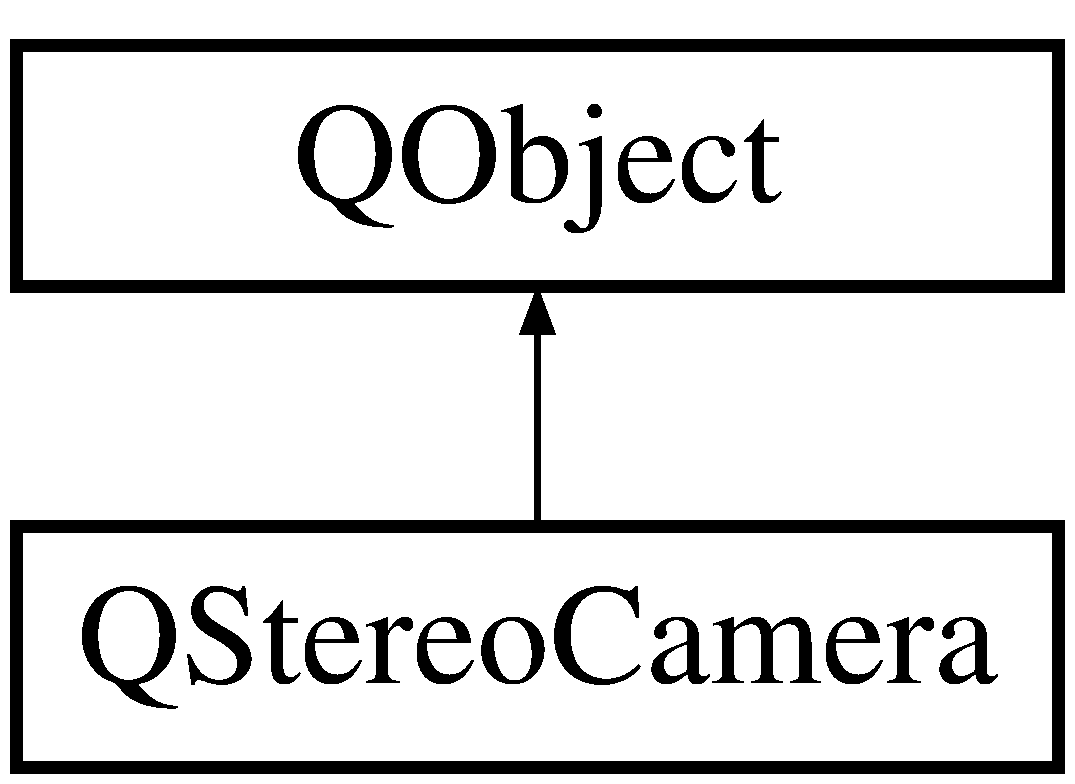
\includegraphics[height=2.000000cm]{class_q_stereo_camera}
\end{center}
\end{figure}
\subsection*{Public Slots}
\begin{DoxyCompactItemize}
\item 
\hypertarget{class_q_stereo_camera_ad4c4726e163c343e86db8d0e7ba4f93c}{}bool {\bfseries set\+Brightness} (int brightness)\label{class_q_stereo_camera_ad4c4726e163c343e86db8d0e7ba4f93c}

\item 
\hypertarget{class_q_stereo_camera_a5d2b6eee1d2f0e881268af5e537f38f7}{}bool {\bfseries set\+Frame\+Size} (int width, int height)\label{class_q_stereo_camera_a5d2b6eee1d2f0e881268af5e537f38f7}

\item 
\hypertarget{class_q_stereo_camera_afa1ecf20b3ac6208da7575cf9fec81b1}{}bool {\bfseries set\+Frame16} (void)\label{class_q_stereo_camera_afa1ecf20b3ac6208da7575cf9fec81b1}

\item 
\hypertarget{class_q_stereo_camera_a8c5d6580c83c7e20a951d0ac879306e1}{}void {\bfseries capture} (void)\label{class_q_stereo_camera_a8c5d6580c83c7e20a951d0ac879306e1}

\item 
\hypertarget{class_q_stereo_camera_adbeac51ba83c6286d5d5985837c15b69}{}void {\bfseries freerun} (void)\label{class_q_stereo_camera_adbeac51ba83c6286d5d5985837c15b69}

\item 
\hypertarget{class_q_stereo_camera_a5dda44ada727369825e774b9d469b408}{}void {\bfseries pause} (void)\label{class_q_stereo_camera_a5dda44ada727369825e774b9d469b408}

\item 
\hypertarget{class_q_stereo_camera_a29dc0fc560511414b6e534d68d54ce81}{}void {\bfseries single\+Shot} (void)\label{class_q_stereo_camera_a29dc0fc560511414b6e534d68d54ce81}

\item 
\hypertarget{class_q_stereo_camera_affc508dcce0294ff148cf1d0ee7d611e}{}bool {\bfseries load\+Calibration} (Q\+String directory)\label{class_q_stereo_camera_affc508dcce0294ff148cf1d0ee7d611e}

\item 
\hypertarget{class_q_stereo_camera_ae8118d48724d1541ded51b924dfa44e2}{}bool {\bfseries load\+Rectification\+Maps} (Q\+String src\+\_\+l, Q\+String src\+\_\+r)\label{class_q_stereo_camera_ae8118d48724d1541ded51b924dfa44e2}

\item 
\hypertarget{class_q_stereo_camera_aba9d75f6f94cc2940321db89a8965aa9}{}void {\bfseries request\+Single} (void)\label{class_q_stereo_camera_aba9d75f6f94cc2940321db89a8965aa9}

\item 
\hypertarget{class_q_stereo_camera_a09667f67f3c092c86ef57191774fc54f}{}void {\bfseries save\+Image} (Q\+String fname)\label{class_q_stereo_camera_a09667f67f3c092c86ef57191774fc54f}

\item 
\hypertarget{class_q_stereo_camera_abddae1c615d05ffe99157246dffab3bf}{}void {\bfseries remap\+\_\+parallel} (cv\+::\+Mat, cv\+::\+Mat \&, cv\+::\+Mat, cv\+::\+Mat)\label{class_q_stereo_camera_abddae1c615d05ffe99157246dffab3bf}

\item 
\hypertarget{class_q_stereo_camera_a4eacb1ad6ae4894f7c1217817ae6a5b1}{}void {\bfseries reproject3\+D} ()\label{class_q_stereo_camera_a4eacb1ad6ae4894f7c1217817ae6a5b1}

\item 
\hypertarget{class_q_stereo_camera_ac8b2af9c26a781d590b6e2fcef243dd5}{}void {\bfseries enable\+Stereo} (bool)\label{class_q_stereo_camera_ac8b2af9c26a781d590b6e2fcef243dd5}

\item 
\hypertarget{class_q_stereo_camera_ac1fb3bbffb92e25ada482507933559f3}{}bool {\bfseries load\+Calibration} (Q\+String left\+\_\+cal, Q\+String right\+\_\+cal, Q\+String stereo\+\_\+cal)\label{class_q_stereo_camera_ac1fb3bbffb92e25ada482507933559f3}

\item 
\hypertarget{class_q_stereo_camera_abe84b80ad1aa56490f266568e57b7758}{}void {\bfseries enable\+Rectify} (bool enable)\label{class_q_stereo_camera_abe84b80ad1aa56490f266568e57b7758}

\item 
\hypertarget{class_q_stereo_camera_a9527e512bd5667a9702a65bb4255319d}{}void {\bfseries match} (void)\label{class_q_stereo_camera_a9527e512bd5667a9702a65bb4255319d}

\item 
\hypertarget{class_q_stereo_camera_ae9da43ba9c4b87cc206932fb011499f8}{}void {\bfseries match\+B\+M} (void)\label{class_q_stereo_camera_ae9da43ba9c4b87cc206932fb011499f8}

\item 
\hypertarget{class_q_stereo_camera_aa4ffccf0f4c98a1a37f8664e9207a4bf}{}void {\bfseries match\+Cuda\+B\+P} (void)\label{class_q_stereo_camera_aa4ffccf0f4c98a1a37f8664e9207a4bf}

\item 
\hypertarget{class_q_stereo_camera_ae4741706dc72c5be061c6ca218e1ad05}{}void {\bfseries match\+S\+G\+B\+M} (void)\label{class_q_stereo_camera_ae4741706dc72c5be061c6ca218e1ad05}

\item 
\hypertarget{class_q_stereo_camera_add46dbf7859730fa50a4cc83dc886974}{}void {\bfseries match\+Cuda\+B\+M} (void)\label{class_q_stereo_camera_add46dbf7859730fa50a4cc83dc886974}

\item 
\hypertarget{class_q_stereo_camera_a248782fdebc3cdf41420b3d84659977b}{}void {\bfseries set\+Matcher} (Q\+String matcher)\label{class_q_stereo_camera_a248782fdebc3cdf41420b3d84659977b}

\item 
\hypertarget{class_q_stereo_camera_aabf3ecce7eb18bb01bb112d777f10776}{}void {\bfseries set\+Matcher\+Pre\+Filter\+Cap} (int pfc)\label{class_q_stereo_camera_aabf3ecce7eb18bb01bb112d777f10776}

\item 
\hypertarget{class_q_stereo_camera_a803f534dac5c97cc917d2b4496dfdf17}{}void {\bfseries set\+Matcher\+Min\+Disparity} (int mindisp)\label{class_q_stereo_camera_a803f534dac5c97cc917d2b4496dfdf17}

\item 
\hypertarget{class_q_stereo_camera_aa64c0dde412216add90face6405f2271}{}void {\bfseries set\+Matcher\+Max\+Disparity} (int maxdisp)\label{class_q_stereo_camera_aa64c0dde412216add90face6405f2271}

\item 
\hypertarget{class_q_stereo_camera_aee2bf5eea7c676d667259d42a78df576}{}void {\bfseries set\+Matcher\+Texture\+Threshold} (int threshold)\label{class_q_stereo_camera_aee2bf5eea7c676d667259d42a78df576}

\item 
\hypertarget{class_q_stereo_camera_a722a9df6ecd425106dd8b8e893bbad06}{}void {\bfseries set\+Matcher\+Block\+Size} (int blocksize)\label{class_q_stereo_camera_a722a9df6ecd425106dd8b8e893bbad06}

\item 
\hypertarget{class_q_stereo_camera_a4cbadff365cabfff41667b1d915a6a54}{}void {\bfseries set\+Matcher\+Speckle\+Window} (int window)\label{class_q_stereo_camera_a4cbadff365cabfff41667b1d915a6a54}

\item 
\hypertarget{class_q_stereo_camera_a0343c15d9652e1729b377a76b195bee0}{}void {\bfseries set\+Matcher\+Speckle\+Range} (int range)\label{class_q_stereo_camera_a0343c15d9652e1729b377a76b195bee0}

\item 
\hypertarget{class_q_stereo_camera_a2ffd4235ca37b72c90ccaa8946b03688}{}void {\bfseries set\+Matcher\+Consistency} (int diff)\label{class_q_stereo_camera_a2ffd4235ca37b72c90ccaa8946b03688}

\item 
\hypertarget{class_q_stereo_camera_af5a66813cc378c0c482a83cab0f66690}{}void {\bfseries set\+Matcher\+Uniqueness} (int uniqueness)\label{class_q_stereo_camera_af5a66813cc378c0c482a83cab0f66690}

\item 
\hypertarget{class_q_stereo_camera_adfb5a91f2209d591da32c1aea590e625}{}void {\bfseries set\+Filter\+Lambda} (int lambda)\label{class_q_stereo_camera_adfb5a91f2209d591da32c1aea590e625}

\item 
\hypertarget{class_q_stereo_camera_a2d580722c27b8b5db9f98cc5ea205383}{}void {\bfseries set\+Filter\+Consistency} (int consistency)\label{class_q_stereo_camera_a2d580722c27b8b5db9f98cc5ea205383}

\item 
\hypertarget{class_q_stereo_camera_ad340b1d66ae85e58ea6d0b7358345f96}{}void {\bfseries set\+Filter\+Sigma\+Colour} (double sigma)\label{class_q_stereo_camera_ad340b1d66ae85e58ea6d0b7358345f96}

\item 
\hypertarget{class_q_stereo_camera_a504569ad87a1c84ad24f4cbb293c418f}{}void {\bfseries set\+Filter\+Discontinuity} (int discontinuity)\label{class_q_stereo_camera_a504569ad87a1c84ad24f4cbb293c418f}

\item 
\hypertarget{class_q_stereo_camera_ac6df8d763e9a3b5454d5fe070130c807}{}void {\bfseries toggle\+Filter} (bool state)\label{class_q_stereo_camera_ac6df8d763e9a3b5454d5fe070130c807}

\item 
\hypertarget{class_q_stereo_camera_a3e1379cb2eb879ad97b14543346a3c84}{}void {\bfseries set\+Savelocation} (Q\+String dir)\label{class_q_stereo_camera_a3e1379cb2eb879ad97b14543346a3c84}

\item 
\hypertarget{class_q_stereo_camera_a132cd9e1cf556224fd33a3b4385d351b}{}bool {\bfseries init\+Video\+Stream} (cv\+::\+Video\+Writer $\ast$writer, Q\+String filename, cv\+::\+Size imsize, double fps=60.\+0, int codec=C\+V\+\_\+\+F\+O\+U\+R\+C\+C('h', '2', '6', '4'))\label{class_q_stereo_camera_a132cd9e1cf556224fd33a3b4385d351b}

\item 
\hypertarget{class_q_stereo_camera_acacdf21f4b8833f672407f3465bd67a0}{}void {\bfseries capture\+Video} (Q\+String fname=\char`\"{}\char`\"{})\label{class_q_stereo_camera_acacdf21f4b8833f672407f3465bd67a0}

\item 
\hypertarget{class_q_stereo_camera_aa1841d6cfb8d6a6bf5e1a15bb9d6d085}{}void {\bfseries stop\+Capture\+Video} (void)\label{class_q_stereo_camera_aa1841d6cfb8d6a6bf5e1a15bb9d6d085}

\end{DoxyCompactItemize}
\subsection*{Signals}
\begin{DoxyCompactItemize}
\item 
\hypertarget{class_q_stereo_camera_afd921962e619a3204db821a1dbfb121f}{}void {\bfseries acquired} ()\label{class_q_stereo_camera_afd921962e619a3204db821a1dbfb121f}

\item 
\hypertarget{class_q_stereo_camera_a9a3e5a73c9ba70ff0e2d3b876af02bce}{}void {\bfseries fps} (qint64)\label{class_q_stereo_camera_a9a3e5a73c9ba70ff0e2d3b876af02bce}

\item 
\hypertarget{class_q_stereo_camera_a139693f1d2b3b434948083a5e8f92b7a}{}void {\bfseries saved\+Image} ()\label{class_q_stereo_camera_a139693f1d2b3b434948083a5e8f92b7a}

\item 
\hypertarget{class_q_stereo_camera_aa9f00a033e7464042162913b2fdd0432}{}void {\bfseries finished} ()\label{class_q_stereo_camera_aa9f00a033e7464042162913b2fdd0432}

\item 
\hypertarget{class_q_stereo_camera_abdacf69cb8b3931e9e0d04d291675d02}{}void {\bfseries framecount} (qint64)\label{class_q_stereo_camera_abdacf69cb8b3931e9e0d04d291675d02}

\item 
\hypertarget{class_q_stereo_camera_acde6c58b457b31fb634b42551bcc2207}{}void {\bfseries saved\+Image} (Q\+String)\label{class_q_stereo_camera_acde6c58b457b31fb634b42551bcc2207}

\item 
\hypertarget{class_q_stereo_camera_aeb01d4039bbadb7c65806f2290e40848}{}void {\bfseries matched} ()\label{class_q_stereo_camera_aeb01d4039bbadb7c65806f2290e40848}

\item 
\hypertarget{class_q_stereo_camera_aaf82430abafe5ed67ba8f2fac163ac97}{}void {\bfseries got\+Point\+Cloud} ()\label{class_q_stereo_camera_aaf82430abafe5ed67ba8f2fac163ac97}

\end{DoxyCompactItemize}
\subsection*{Public Member Functions}
\begin{DoxyCompactItemize}
\item 
\hypertarget{class_q_stereo_camera_a9fc87c0fb63f5f1dc051bef6d0e1718b}{}{\bfseries Q\+Stereo\+Camera} (Q\+Object $\ast$parent=0)\label{class_q_stereo_camera_a9fc87c0fb63f5f1dc051bef6d0e1718b}

\item 
\hypertarget{class_q_stereo_camera_a7a74b825ee958be9130990fdd3165b02}{}void {\bfseries assign\+Thread} (Q\+Thread $\ast$thread)\label{class_q_stereo_camera_a7a74b825ee958be9130990fdd3165b02}

\item 
\hypertarget{class_q_stereo_camera_a1c604e29157167d67f6a80b50f5e2d3e}{}bool {\bfseries init} (void)\label{class_q_stereo_camera_a1c604e29157167d67f6a80b50f5e2d3e}

\item 
\hypertarget{class_q_stereo_camera_abce4b7d10c518ef49a989c28ea9a18f7}{}int {\bfseries get\+Exposure} (void)\label{class_q_stereo_camera_abce4b7d10c518ef49a989c28ea9a18f7}

\item 
\hypertarget{class_q_stereo_camera_a074b6b7b89d1ae0405a25e6e5ceabc0a}{}bool {\bfseries is\+Acquiring} (void)\label{class_q_stereo_camera_a074b6b7b89d1ae0405a25e6e5ceabc0a}

\item 
\hypertarget{class_q_stereo_camera_aca3c6fa7d94024cbc761782aac469541}{}void {\bfseries match\+Impact} (void)\label{class_q_stereo_camera_aca3c6fa7d94024cbc761782aac469541}

\end{DoxyCompactItemize}
\subsection*{Public Attributes}
\begin{DoxyCompactItemize}
\item 
\hypertarget{class_q_stereo_camera_a82eeb68a3c2e506ccf5200774abedb2d}{}cv\+::\+Mat {\bfseries channels} \mbox{[}3\mbox{]}\label{class_q_stereo_camera_a82eeb68a3c2e506ccf5200774abedb2d}

\item 
\hypertarget{class_q_stereo_camera_a5b1c7aad19620151a9af4aac4d91f13a}{}cv\+::\+Mat {\bfseries left\+\_\+remapped}\label{class_q_stereo_camera_a5b1c7aad19620151a9af4aac4d91f13a}

\item 
\hypertarget{class_q_stereo_camera_a0687947a6f63f41970f591e88f445126}{}cv\+::\+Mat {\bfseries right\+\_\+remapped}\label{class_q_stereo_camera_a0687947a6f63f41970f591e88f445126}

\item 
\hypertarget{class_q_stereo_camera_a67b6fb7641cd8ee700a40dfbd92bed2e}{}cv\+::\+Mat {\bfseries stereo\+\_\+out}\label{class_q_stereo_camera_a67b6fb7641cd8ee700a40dfbd92bed2e}

\item 
\hypertarget{class_q_stereo_camera_accd16386026a96e7080e8ad4d5d3aad9}{}cv\+::\+Mat {\bfseries left\+\_\+raw}\label{class_q_stereo_camera_accd16386026a96e7080e8ad4d5d3aad9}

\item 
\hypertarget{class_q_stereo_camera_af038e1b4ffeec640ce7e8093689c9e3a}{}cv\+::\+Mat {\bfseries right\+\_\+raw}\label{class_q_stereo_camera_af038e1b4ffeec640ce7e8093689c9e3a}

\item 
\hypertarget{class_q_stereo_camera_af198164a2259de179bed4eed61fa1e73}{}cv\+::\+Mat {\bfseries r\+\_\+camera\+\_\+matrix}\label{class_q_stereo_camera_af198164a2259de179bed4eed61fa1e73}

\item 
\hypertarget{class_q_stereo_camera_ac5b7f2810a93660828319d08cb161901}{}cv\+::\+Mat {\bfseries l\+\_\+camera\+\_\+matrix}\label{class_q_stereo_camera_ac5b7f2810a93660828319d08cb161901}

\item 
\hypertarget{class_q_stereo_camera_ad59550fab715a35fb31d2fcface31f69}{}cv\+::\+Mat {\bfseries l\+\_\+dist\+\_\+coeffs}\label{class_q_stereo_camera_ad59550fab715a35fb31d2fcface31f69}

\item 
\hypertarget{class_q_stereo_camera_ae60ae5320f8cc33507b5d4c55b108317}{}cv\+::\+Mat {\bfseries r\+\_\+dist\+\_\+coeffs}\label{class_q_stereo_camera_ae60ae5320f8cc33507b5d4c55b108317}

\item 
\hypertarget{class_q_stereo_camera_ab115211419ed1dd0953b4aabfd7039b9}{}cv\+::\+Mat {\bfseries Q}\label{class_q_stereo_camera_ab115211419ed1dd0953b4aabfd7039b9}

\item 
\hypertarget{class_q_stereo_camera_aaa6194f9f12be746674fb356b0b7190a}{}pcl\+::\+Point\+Cloud$<$ pcl\+::\+Point\+X\+Y\+Z\+R\+G\+B $>$\+::Ptr {\bfseries pt\+Cloud}\label{class_q_stereo_camera_aaa6194f9f12be746674fb356b0b7190a}

\item 
\hypertarget{class_q_stereo_camera_aaccb16ea0cdf6bf2a01e5f6f38d09940}{}Q\+String {\bfseries save\+Dir} = \char`\"{}.\char`\"{}\label{class_q_stereo_camera_aaccb16ea0cdf6bf2a01e5f6f38d09940}

\item 
\hypertarget{class_q_stereo_camera_a5ce524846bec1143c6f4c648e2dd5d75}{}int {\bfseries image\+Width}\label{class_q_stereo_camera_a5ce524846bec1143c6f4c648e2dd5d75}

\item 
\hypertarget{class_q_stereo_camera_aa8c9d1b89f7975757d4b8e899147f294}{}int {\bfseries image\+Height}\label{class_q_stereo_camera_aa8c9d1b89f7975757d4b8e899147f294}

\end{DoxyCompactItemize}


\subsection{Detailed Description}


Definition at line 41 of file qstereocamera.\+h.



The documentation for this class was generated from the following files\+:\begin{DoxyCompactItemize}
\item 
src/qstereocamera.\+h\item 
src/qstereocamera.\+cpp\end{DoxyCompactItemize}

\hypertarget{class_stereo_calibrate}{}\section{Stereo\+Calibrate Class Reference}
\label{class_stereo_calibrate}\index{Stereo\+Calibrate@{Stereo\+Calibrate}}
Inheritance diagram for Stereo\+Calibrate\+:\begin{figure}[H]
\begin{center}
\leavevmode
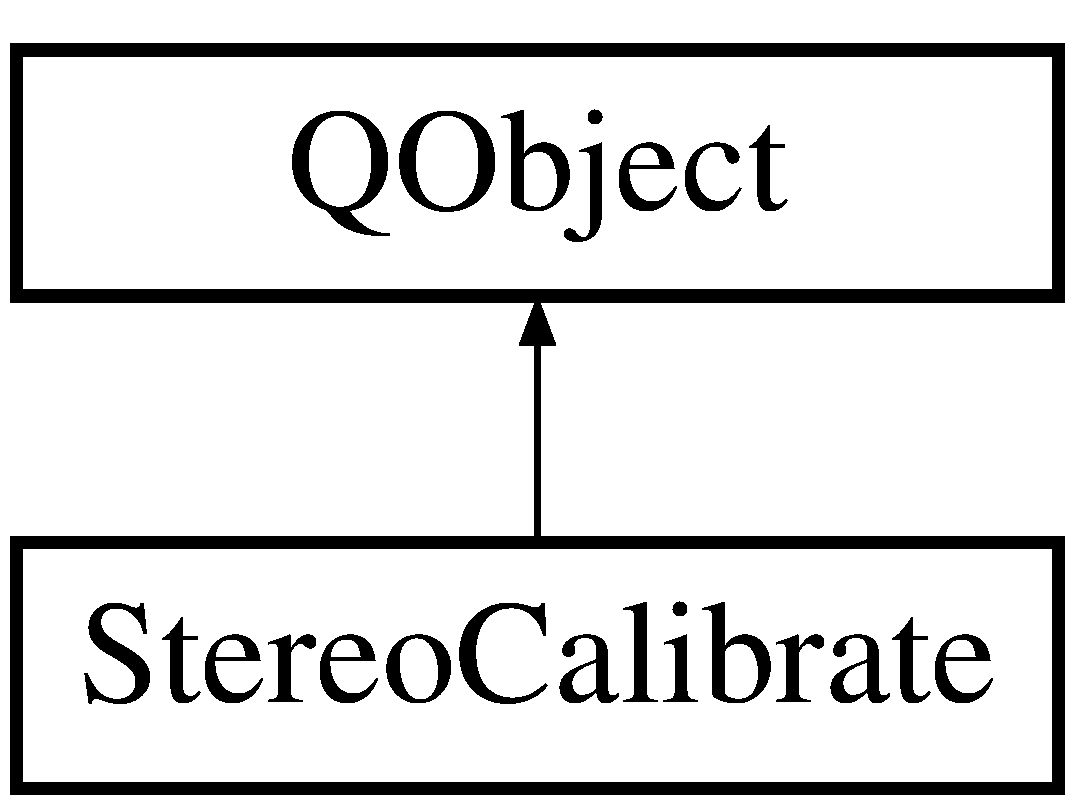
\includegraphics[height=2.000000cm]{class_stereo_calibrate}
\end{center}
\end{figure}
\subsection*{Public Slots}
\begin{DoxyCompactItemize}
\item 
\hypertarget{class_stereo_calibrate_a6e4b4838382adcf8a2cb27b9f37eb110}{}void {\bfseries abort\+Calibration} ()\label{class_stereo_calibrate_a6e4b4838382adcf8a2cb27b9f37eb110}

\item 
\hypertarget{class_stereo_calibrate_a9bab18de2d9dc031100a427f5ffd3124}{}void {\bfseries set\+Displays} (Q\+Label $\ast$left, Q\+Label $\ast$right)\label{class_stereo_calibrate_a9bab18de2d9dc031100a427f5ffd3124}

\item 
\hypertarget{class_stereo_calibrate_ac474055fd6fe2e6072ea0f064e2e42ac}{}void {\bfseries set\+Board\+Orientations} (std\+::vector$<$ \hyperlink{class_chessboard}{Chessboard} $\ast$ $>$ \&orientations)\label{class_stereo_calibrate_ac474055fd6fe2e6072ea0f064e2e42ac}

\item 
\hypertarget{class_stereo_calibrate_a2e3e6d6b3d6de2c593adc57108c265fc}{}void {\bfseries update\+Views} (void)\label{class_stereo_calibrate_a2e3e6d6b3d6de2c593adc57108c265fc}

\item 
\hypertarget{class_stereo_calibrate_aef3fbab18b6c999aa22f06a1f238114e}{}void {\bfseries start\+Calibration} (void)\label{class_stereo_calibrate_aef3fbab18b6c999aa22f06a1f238114e}

\item 
\hypertarget{class_stereo_calibrate_a69e4719c556f500027651b6fc9648f3a}{}void {\bfseries check\+Images} (void)\label{class_stereo_calibrate_a69e4719c556f500027651b6fc9648f3a}

\item 
\hypertarget{class_stereo_calibrate_a579036077efc510864e55ead9e479376}{}void {\bfseries load\+Board\+Poses} (std\+::string fname)\label{class_stereo_calibrate_a579036077efc510864e55ead9e479376}

\item 
\hypertarget{class_stereo_calibrate_a315e6d7c92a006003242ae548f56ca29}{}bool {\bfseries image\+Valid} (void)\label{class_stereo_calibrate_a315e6d7c92a006003242ae548f56ca29}

\item 
\hypertarget{class_stereo_calibrate_acd9488fed7fbb75f1b74f3d5757bbef7}{}void {\bfseries overlay\+Image} (cv\+::\+Mat \&image, \hyperlink{class_chessboard}{Chessboard} $\ast$board=0, bool found=false, bool valid=false)\label{class_stereo_calibrate_acd9488fed7fbb75f1b74f3d5757bbef7}

\item 
\hypertarget{class_stereo_calibrate_a09d1ae49ef40584e222c977548bd74f8}{}void {\bfseries set\+Images} (Q\+List$<$ Q\+String $>$ left, Q\+List$<$ Q\+String $>$ right)\label{class_stereo_calibrate_a09d1ae49ef40584e222c977548bd74f8}

\item 
\hypertarget{class_stereo_calibrate_ae5859fd10b2abc8f9c6c46191199c9fb}{}void {\bfseries set\+Pattern} (cv\+::\+Size size, double square\+Size)\label{class_stereo_calibrate_ae5859fd10b2abc8f9c6c46191199c9fb}

\item 
\hypertarget{class_stereo_calibrate_ab7e823429a93bfc6b922b0250963a3f5}{}void {\bfseries set\+Image\+Size} (cv\+::\+Size size)\label{class_stereo_calibrate_ab7e823429a93bfc6b922b0250963a3f5}

\item 
\hypertarget{class_stereo_calibrate_a96b0cb2c8b225d1c7373f235d614f4a9}{}void {\bfseries overlay\+Arrow} (cv\+::\+Mat \&image, std\+::vector$<$ cv\+::\+Point2f $>$ \&points, cv\+::\+Point2f offset, Cv\+Scalar colour, int thickness=3)\label{class_stereo_calibrate_a96b0cb2c8b225d1c7373f235d614f4a9}

\item 
\hypertarget{class_stereo_calibrate_aac7cce8c777aff0eb5773804718c7f89}{}bool {\bfseries joint\+Calibration} (void)\label{class_stereo_calibrate_aac7cce8c777aff0eb5773804718c7f89}

\end{DoxyCompactItemize}
\subsection*{Signals}
\begin{DoxyCompactItemize}
\item 
\hypertarget{class_stereo_calibrate_ac3d8097c8d6a5c9fe8c97439716f13e7}{}void {\bfseries done\+Calibration} (bool)\label{class_stereo_calibrate_ac3d8097c8d6a5c9fe8c97439716f13e7}

\item 
\hypertarget{class_stereo_calibrate_a41525653d38ca4e2a45a6daf5dc45f08}{}void {\bfseries image\+Progress} (int, int)\label{class_stereo_calibrate_a41525653d38ca4e2a45a6daf5dc45f08}

\item 
\hypertarget{class_stereo_calibrate_ab1db6cd7acd48f9c7a34a76ce6aca340}{}void {\bfseries request\+Image} (void)\label{class_stereo_calibrate_ab1db6cd7acd48f9c7a34a76ce6aca340}

\item 
\hypertarget{class_stereo_calibrate_a3408cbc47f9926c5505cab7a0e0e7ddc}{}void {\bfseries chessboard\+Found} (\hyperlink{class_chessboard}{Chessboard} $\ast$board)\label{class_stereo_calibrate_a3408cbc47f9926c5505cab7a0e0e7ddc}

\item 
\hypertarget{class_stereo_calibrate_a29a79921e046abe6d70012c93a18533c}{}void {\bfseries done\+\_\+image} (int i)\label{class_stereo_calibrate_a29a79921e046abe6d70012c93a18533c}

\end{DoxyCompactItemize}
\subsection*{Public Member Functions}
\begin{DoxyCompactItemize}
\item 
\hypertarget{class_stereo_calibrate_a0ba54ebc21eea32ab13ced8731dd4423}{}{\bfseries Stereo\+Calibrate} (Q\+Object $\ast$parent=0, \hyperlink{class_abstract_stereo_camera}{Abstract\+Stereo\+Camera} $\ast$stereo\+\_\+camera=0)\label{class_stereo_calibrate_a0ba54ebc21eea32ab13ced8731dd4423}

\end{DoxyCompactItemize}
\subsection*{Public Attributes}
\begin{DoxyCompactItemize}
\item 
\hypertarget{class_stereo_calibrate_a08c3badac3bd497e657aff56403d3ef2}{}cv\+::\+Mat {\bfseries left\+\_\+camera\+\_\+matrix}\label{class_stereo_calibrate_a08c3badac3bd497e657aff56403d3ef2}

\item 
\hypertarget{class_stereo_calibrate_a4439722cdafcbeb128a327d5603a1d82}{}cv\+::\+Mat {\bfseries left\+\_\+distortion}\label{class_stereo_calibrate_a4439722cdafcbeb128a327d5603a1d82}

\item 
\hypertarget{class_stereo_calibrate_a9fa4c7b35474447f2c2641b0a582d2a4}{}cv\+::\+Mat {\bfseries left\+\_\+r\+\_\+vecs}\label{class_stereo_calibrate_a9fa4c7b35474447f2c2641b0a582d2a4}

\item 
\hypertarget{class_stereo_calibrate_a70310138b5d79e790b59e9cd902cc8ee}{}cv\+::\+Mat {\bfseries left\+\_\+t\+\_\+vecs}\label{class_stereo_calibrate_a70310138b5d79e790b59e9cd902cc8ee}

\item 
\hypertarget{class_stereo_calibrate_a332c1a0d65ead579635cf4097cd0dad5}{}double {\bfseries left\+\_\+rms\+\_\+error}\label{class_stereo_calibrate_a332c1a0d65ead579635cf4097cd0dad5}

\item 
\hypertarget{class_stereo_calibrate_ad4a81b056b4b92c75fa9c2865a9a10d9}{}cv\+::\+Mat {\bfseries right\+\_\+camera\+\_\+matrix}\label{class_stereo_calibrate_ad4a81b056b4b92c75fa9c2865a9a10d9}

\item 
\hypertarget{class_stereo_calibrate_a02d2fbfd18e1760134161e77a18f01c2}{}cv\+::\+Mat {\bfseries right\+\_\+distortion}\label{class_stereo_calibrate_a02d2fbfd18e1760134161e77a18f01c2}

\item 
\hypertarget{class_stereo_calibrate_a7459460dfaee56361e062e09df457462}{}cv\+::\+Mat {\bfseries right\+\_\+r\+\_\+vecs}\label{class_stereo_calibrate_a7459460dfaee56361e062e09df457462}

\item 
\hypertarget{class_stereo_calibrate_a18f0b17f3ef22b1b1e2f8d8de627840e}{}cv\+::\+Mat {\bfseries right\+\_\+t\+\_\+vecs}\label{class_stereo_calibrate_a18f0b17f3ef22b1b1e2f8d8de627840e}

\item 
\hypertarget{class_stereo_calibrate_a65d2c639e6d75e4955d59d251431ddd0}{}double {\bfseries right\+\_\+rms\+\_\+error}\label{class_stereo_calibrate_a65d2c639e6d75e4955d59d251431ddd0}

\item 
\hypertarget{class_stereo_calibrate_aeb574c601840e023ac3bcada4c43d71b}{}cv\+::\+Mat {\bfseries stereo\+\_\+r}\label{class_stereo_calibrate_aeb574c601840e023ac3bcada4c43d71b}

\item 
\hypertarget{class_stereo_calibrate_aa4d8872e0c9d353d3d85dbd679e1153b}{}cv\+::\+Mat {\bfseries stereo\+\_\+t}\label{class_stereo_calibrate_aa4d8872e0c9d353d3d85dbd679e1153b}

\item 
\hypertarget{class_stereo_calibrate_ae47284ab43d5edb77bb09ec0d415daf5}{}cv\+::\+Mat {\bfseries stereo\+\_\+e}\label{class_stereo_calibrate_ae47284ab43d5edb77bb09ec0d415daf5}

\item 
\hypertarget{class_stereo_calibrate_a9683503b4ff3d2db1a9266a6a7837497}{}cv\+::\+Mat {\bfseries stereo\+\_\+f}\label{class_stereo_calibrate_a9683503b4ff3d2db1a9266a6a7837497}

\item 
\hypertarget{class_stereo_calibrate_ae684e6f92a70b3f4684d205cfca11463}{}cv\+::\+Mat {\bfseries stereo\+\_\+q}\label{class_stereo_calibrate_ae684e6f92a70b3f4684d205cfca11463}

\item 
\hypertarget{class_stereo_calibrate_a9904403fff5a29e885b8cb7df65e8df4}{}double {\bfseries stereo\+\_\+rms\+\_\+error}\label{class_stereo_calibrate_a9904403fff5a29e885b8cb7df65e8df4}

\item 
\hypertarget{class_stereo_calibrate_a38717dfe41458f60fc249e3a26fc21c4}{}cv\+::\+Mat {\bfseries left\+\_\+rectification\+\_\+x}\label{class_stereo_calibrate_a38717dfe41458f60fc249e3a26fc21c4}

\item 
\hypertarget{class_stereo_calibrate_a346a6e37301f5b4b45cacd7977c21b7d}{}cv\+::\+Mat {\bfseries left\+\_\+rectification\+\_\+y}\label{class_stereo_calibrate_a346a6e37301f5b4b45cacd7977c21b7d}

\item 
\hypertarget{class_stereo_calibrate_acb56d8421682bba175433ef4538dc7a5}{}cv\+::\+Mat {\bfseries right\+\_\+rectification\+\_\+x}\label{class_stereo_calibrate_acb56d8421682bba175433ef4538dc7a5}

\item 
\hypertarget{class_stereo_calibrate_ade96b91d120281da9e789d95f7f33902}{}cv\+::\+Mat {\bfseries right\+\_\+rectification\+\_\+y}\label{class_stereo_calibrate_ade96b91d120281da9e789d95f7f33902}

\end{DoxyCompactItemize}


\subsection{Detailed Description}


Definition at line 23 of file stereocalibrate.\+h.



The documentation for this class was generated from the following files\+:\begin{DoxyCompactItemize}
\item 
src/stereocalibrate.\+h\item 
src/stereocalibrate.\+cpp\end{DoxyCompactItemize}

\hypertarget{class_stereo_camera_deimos}{}\section{Stereo\+Camera\+Deimos Class Reference}
\label{class_stereo_camera_deimos}\index{Stereo\+Camera\+Deimos@{Stereo\+Camera\+Deimos}}
Inheritance diagram for Stereo\+Camera\+Deimos\+:\begin{figure}[H]
\begin{center}
\leavevmode
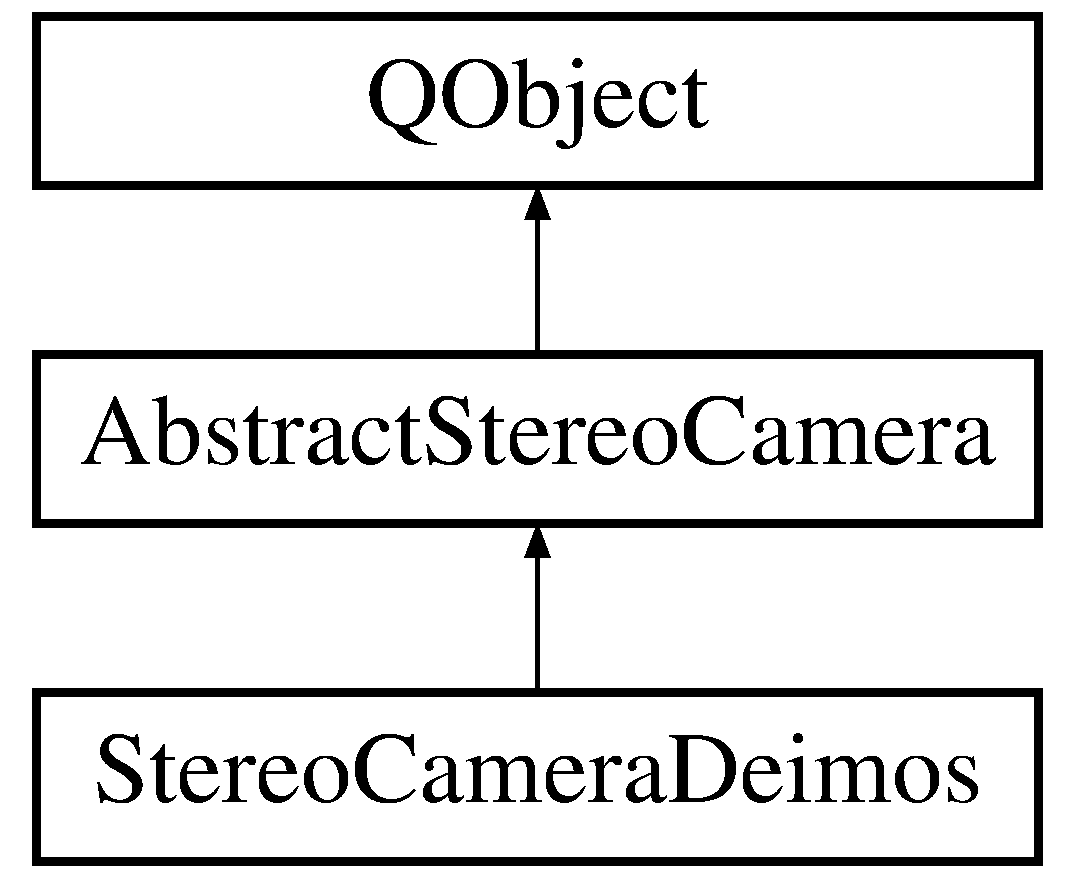
\includegraphics[height=3.000000cm]{class_stereo_camera_deimos}
\end{center}
\end{figure}
\subsection*{Public Slots}
\begin{DoxyCompactItemize}
\item 
\hypertarget{class_stereo_camera_deimos_a2033de5e607f874b8c5e78b79d17e16e}{}bool {\bfseries set\+Exposure} (double exposure\+\_\+time)\label{class_stereo_camera_deimos_a2033de5e607f874b8c5e78b79d17e16e}

\item 
\hypertarget{class_stereo_camera_deimos_a755406c93b4ffd2ef58a4fc61d7c3ffd}{}bool {\bfseries toggle\+H\+D\+R} (bool enable)\label{class_stereo_camera_deimos_a755406c93b4ffd2ef58a4fc61d7c3ffd}

\item 
\hypertarget{class_stereo_camera_deimos_aa29a36f98a63e0550f25c8f8b871fee0}{}bool {\bfseries enable\+Auto\+Expose} (bool enable)\label{class_stereo_camera_deimos_aa29a36f98a63e0550f25c8f8b871fee0}

\item 
\hypertarget{class_stereo_camera_deimos_a1eb7eb2521979e1e0d3d899aafd679d4}{}double {\bfseries get\+Temperature} (void)\label{class_stereo_camera_deimos_a1eb7eb2521979e1e0d3d899aafd679d4}

\end{DoxyCompactItemize}
\subsection*{Public Member Functions}
\begin{DoxyCompactItemize}
\item 
\hypertarget{class_stereo_camera_deimos_ae69499b39216ee6b6aa5b2e9512f3c09}{}{\bfseries Stereo\+Camera\+Deimos} (Q\+Object $\ast$parent=0)\label{class_stereo_camera_deimos_ae69499b39216ee6b6aa5b2e9512f3c09}

\item 
bool \hyperlink{class_stereo_camera_deimos_a7526953f7562acc07841ebd6a49dc043}{capture} ()
\begin{DoxyCompactList}\small\item\em Capture an image. \end{DoxyCompactList}\item 
\hypertarget{class_stereo_camera_deimos_a60c865353deac27471bbdc0316099c1b}{}void {\bfseries disconnect\+Camera} ()\label{class_stereo_camera_deimos_a60c865353deac27471bbdc0316099c1b}

\item 
\hypertarget{class_stereo_camera_deimos_a3af4df4317df52f1900f9372d9cbf8bd}{}bool {\bfseries init\+Camera} (int devid=-\/1)\label{class_stereo_camera_deimos_a3af4df4317df52f1900f9372d9cbf8bd}

\item 
\hypertarget{class_stereo_camera_deimos_a64982ba0f3de8f93e3e179f5575496e0}{}int {\bfseries find\+Camera} (void)\label{class_stereo_camera_deimos_a64982ba0f3de8f93e3e179f5575496e0}

\item 
\hypertarget{class_stereo_camera_deimos_a7b6f5773ef6266aa79b5970210e00d71}{}bool {\bfseries set\+Frame\+Size} (int width, int height)\label{class_stereo_camera_deimos_a7b6f5773ef6266aa79b5970210e00d71}

\item 
\hypertarget{class_stereo_camera_deimos_a538f481037c273608cfee38bb714a9f0}{}bool {\bfseries set\+Frame16} (void)\label{class_stereo_camera_deimos_a538f481037c273608cfee38bb714a9f0}

\item 
\hypertarget{class_stereo_camera_deimos_ac734aa162a5994522b5ec4078e6d4d4f}{}void {\bfseries get\+Frame\+Rate} (void)\label{class_stereo_camera_deimos_ac734aa162a5994522b5ec4078e6d4d4f}

\item 
\hypertarget{class_stereo_camera_deimos_a9e40d1909c6552c982b06ed73eb737ba}{}void {\bfseries open\+H\+I\+D} ()\label{class_stereo_camera_deimos_a9e40d1909c6552c982b06ed73eb737ba}

\item 
\hypertarget{class_stereo_camera_deimos_a19578fe34c606f6d40f561b56bc3aad8}{}int {\bfseries get\+Exposure} ()\label{class_stereo_camera_deimos_a19578fe34c606f6d40f561b56bc3aad8}

\end{DoxyCompactItemize}
\subsection*{Additional Inherited Members}


\subsection{Detailed Description}


Definition at line 34 of file stereocameradeimos.\+h.



\subsection{Member Function Documentation}
\hypertarget{class_stereo_camera_deimos_a7526953f7562acc07841ebd6a49dc043}{}\index{Stereo\+Camera\+Deimos@{Stereo\+Camera\+Deimos}!capture@{capture}}
\index{capture@{capture}!Stereo\+Camera\+Deimos@{Stereo\+Camera\+Deimos}}
\subsubsection[{capture}]{\setlength{\rightskip}{0pt plus 5cm}bool Stereo\+Camera\+Deimos\+::capture (
\begin{DoxyParamCaption}
{}
\end{DoxyParamCaption}
)\hspace{0.3cm}{\ttfamily [virtual]}}\label{class_stereo_camera_deimos_a7526953f7562acc07841ebd6a49dc043}


Capture an image. 

This is a virtual function which should be implmeented by a particular camera driver.

\begin{DoxyReturn}{Returns}
True if an image was captured successfully, false otherwise 
\end{DoxyReturn}


Implements \hyperlink{class_abstract_stereo_camera_a01d0ecf3cf4bb8e9a6b9e34292483d14}{Abstract\+Stereo\+Camera}.



Definition at line 323 of file stereocameradeimos.\+cpp.



The documentation for this class was generated from the following files\+:\begin{DoxyCompactItemize}
\item 
src/stereocameradeimos.\+h\item 
src/stereocameradeimos.\+cpp\end{DoxyCompactItemize}

\hypertarget{class_stereo_camera_from_video}{}\section{Stereo\+Camera\+From\+Video Class Reference}
\label{class_stereo_camera_from_video}\index{Stereo\+Camera\+From\+Video@{Stereo\+Camera\+From\+Video}}
Inheritance diagram for Stereo\+Camera\+From\+Video\+:\begin{figure}[H]
\begin{center}
\leavevmode
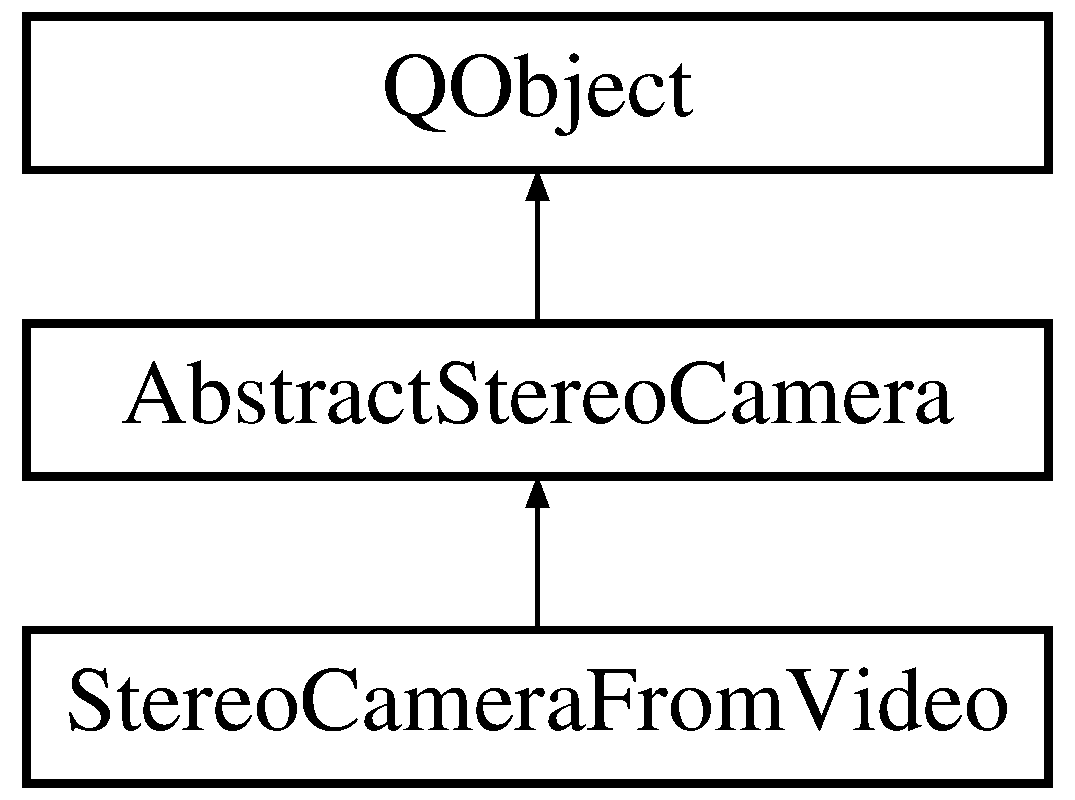
\includegraphics[height=3.000000cm]{class_stereo_camera_from_video}
\end{center}
\end{figure}
\subsection*{Public Slots}
\begin{DoxyCompactItemize}
\item 
\hypertarget{class_stereo_camera_from_video_ab0ea47d4b231ebbc892ca5b51773add9}{}void {\bfseries set\+Position} (int position)\label{class_stereo_camera_from_video_ab0ea47d4b231ebbc892ca5b51773add9}

\item 
\hypertarget{class_stereo_camera_from_video_a3699596ba9de3b2ae1959da6a6097cf3}{}bool {\bfseries enable\+Auto\+Expose} (bool enable)\label{class_stereo_camera_from_video_a3699596ba9de3b2ae1959da6a6097cf3}

\end{DoxyCompactItemize}
\subsection*{Signals}
\begin{DoxyCompactItemize}
\item 
\hypertarget{class_stereo_camera_from_video_ad9a777afd6aede6d23d09e4b86430669}{}void {\bfseries video\+Position} (int)\label{class_stereo_camera_from_video_ad9a777afd6aede6d23d09e4b86430669}

\end{DoxyCompactItemize}
\subsection*{Public Member Functions}
\begin{DoxyCompactItemize}
\item 
\hypertarget{class_stereo_camera_from_video_ae98c29028ab573c2c6d1ddaa104595c9}{}{\bfseries Stereo\+Camera\+From\+Video} (Q\+Object $\ast$parent=0)\label{class_stereo_camera_from_video_ae98c29028ab573c2c6d1ddaa104595c9}

\item 
bool \hyperlink{class_stereo_camera_from_video_af53503df1755c0a9cf84718128ed0a5d}{capture} ()
\begin{DoxyCompactList}\small\item\em Capture an image. \end{DoxyCompactList}\item 
\hypertarget{class_stereo_camera_from_video_a1156dab0196f1366e95f82b3d197eb34}{}void {\bfseries disconnect\+Camera} ()\label{class_stereo_camera_from_video_a1156dab0196f1366e95f82b3d197eb34}

\item 
\hypertarget{class_stereo_camera_from_video_af52f8d11867223d927c6b0f18dd4cdcb}{}bool {\bfseries init\+Camera} (Q\+String fname)\label{class_stereo_camera_from_video_af52f8d11867223d927c6b0f18dd4cdcb}

\end{DoxyCompactItemize}
\subsection*{Additional Inherited Members}


\subsection{Detailed Description}


Definition at line 11 of file stereocamerafromvideo.\+h.



\subsection{Member Function Documentation}
\hypertarget{class_stereo_camera_from_video_af53503df1755c0a9cf84718128ed0a5d}{}\index{Stereo\+Camera\+From\+Video@{Stereo\+Camera\+From\+Video}!capture@{capture}}
\index{capture@{capture}!Stereo\+Camera\+From\+Video@{Stereo\+Camera\+From\+Video}}
\subsubsection[{capture}]{\setlength{\rightskip}{0pt plus 5cm}bool Stereo\+Camera\+From\+Video\+::capture (
\begin{DoxyParamCaption}
{}
\end{DoxyParamCaption}
)\hspace{0.3cm}{\ttfamily [virtual]}}\label{class_stereo_camera_from_video_af53503df1755c0a9cf84718128ed0a5d}


Capture an image. 

This is a virtual function which should be implmeented by a particular camera driver.

\begin{DoxyReturn}{Returns}
True if an image was captured successfully, false otherwise 
\end{DoxyReturn}


Implements \hyperlink{class_abstract_stereo_camera_a01d0ecf3cf4bb8e9a6b9e34292483d14}{Abstract\+Stereo\+Camera}.



Definition at line 41 of file stereocamerafromvideo.\+cpp.



The documentation for this class was generated from the following files\+:\begin{DoxyCompactItemize}
\item 
src/stereocamerafromvideo.\+h\item 
src/stereocamerafromvideo.\+cpp\end{DoxyCompactItemize}

\hypertarget{class_stereo_camera_open_c_v}{}\section{Stereo\+Camera\+Open\+C\+V Class Reference}
\label{class_stereo_camera_open_c_v}\index{Stereo\+Camera\+Open\+C\+V@{Stereo\+Camera\+Open\+C\+V}}
Inheritance diagram for Stereo\+Camera\+Open\+C\+V\+:\begin{figure}[H]
\begin{center}
\leavevmode
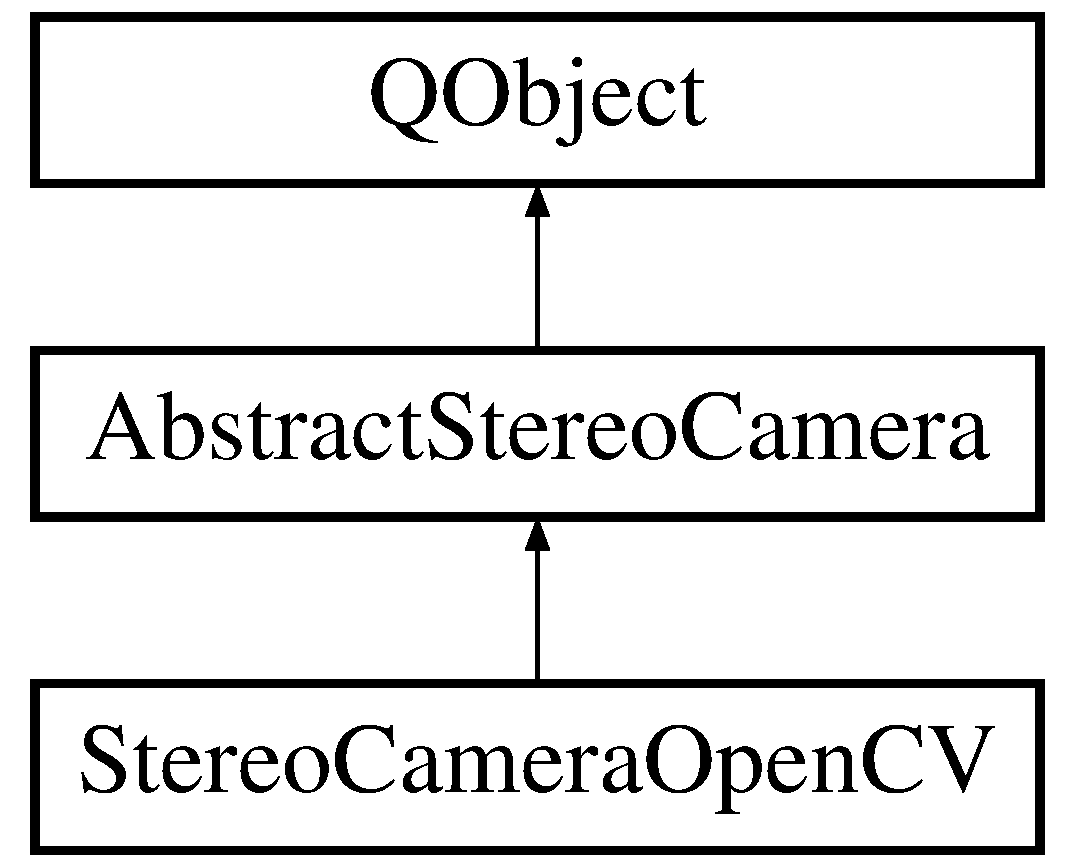
\includegraphics[height=3.000000cm]{class_stereo_camera_open_c_v}
\end{center}
\end{figure}
\subsection*{Public Member Functions}
\begin{DoxyCompactItemize}
\item 
\hypertarget{class_stereo_camera_open_c_v_a719245d43f1ce2f25c875ac9bb7ec6f3}{}{\bfseries Stereo\+Camera\+Open\+C\+V} (Q\+Object $\ast$parent=0)\label{class_stereo_camera_open_c_v_a719245d43f1ce2f25c875ac9bb7ec6f3}

\item 
\hypertarget{class_stereo_camera_open_c_v_a6168a4ae04b223866a8e41365c88aa8e}{}void {\bfseries set\+Devices} (int left\+\_\+index, int right\+\_\+index)\label{class_stereo_camera_open_c_v_a6168a4ae04b223866a8e41365c88aa8e}

\item 
bool \hyperlink{class_stereo_camera_open_c_v_ac669e811da12df2bfd76f783c0550100}{capture} ()
\begin{DoxyCompactList}\small\item\em Capture an image. \end{DoxyCompactList}\item 
\hypertarget{class_stereo_camera_open_c_v_ac09a94c2131ce8b0aa2e4dc743276121}{}void {\bfseries disconnect\+Camera} ()\label{class_stereo_camera_open_c_v_ac09a94c2131ce8b0aa2e4dc743276121}

\item 
\hypertarget{class_stereo_camera_open_c_v_a59c5da56b77dfbfbe94985c196a28777}{}bool {\bfseries init\+Camera} (int left\+\_\+index, int right\+\_\+index)\label{class_stereo_camera_open_c_v_a59c5da56b77dfbfbe94985c196a28777}

\item 
\hypertarget{class_stereo_camera_open_c_v_adf3fb1c866b19ba2fea2ebd36251e075}{}bool {\bfseries init\+Camera} (void)\label{class_stereo_camera_open_c_v_adf3fb1c866b19ba2fea2ebd36251e075}

\item 
\hypertarget{class_stereo_camera_open_c_v_ae6dfcf2aa00ca0f213d2fb0327f23147}{}bool {\bfseries set\+Exposure} (double exposure)\label{class_stereo_camera_open_c_v_ae6dfcf2aa00ca0f213d2fb0327f23147}

\end{DoxyCompactItemize}
\subsection*{Additional Inherited Members}


\subsection{Detailed Description}


Definition at line 13 of file stereocameraopencv.\+h.



\subsection{Member Function Documentation}
\hypertarget{class_stereo_camera_open_c_v_ac669e811da12df2bfd76f783c0550100}{}\index{Stereo\+Camera\+Open\+C\+V@{Stereo\+Camera\+Open\+C\+V}!capture@{capture}}
\index{capture@{capture}!Stereo\+Camera\+Open\+C\+V@{Stereo\+Camera\+Open\+C\+V}}
\subsubsection[{capture}]{\setlength{\rightskip}{0pt plus 5cm}bool Stereo\+Camera\+Open\+C\+V\+::capture (
\begin{DoxyParamCaption}
{}
\end{DoxyParamCaption}
)\hspace{0.3cm}{\ttfamily [virtual]}}\label{class_stereo_camera_open_c_v_ac669e811da12df2bfd76f783c0550100}


Capture an image. 

This is a virtual function which should be implmeented by a particular camera driver.

\begin{DoxyReturn}{Returns}
True if an image was captured successfully, false otherwise 
\end{DoxyReturn}


Implements \hyperlink{class_abstract_stereo_camera_a01d0ecf3cf4bb8e9a6b9e34292483d14}{Abstract\+Stereo\+Camera}.



Definition at line 44 of file stereocameraopencv.\+cpp.



The documentation for this class was generated from the following files\+:\begin{DoxyCompactItemize}
\item 
src/stereocameraopencv.\+h\item 
src/stereocameraopencv.\+cpp\end{DoxyCompactItemize}

%--- End generated contents ---

% Index
\backmatter
\newpage
\phantomsection
\clearemptydoublepage
\addcontentsline{toc}{chapter}{Index}
\printindex

\end{document}
